\documentclass[12pt]{report}
\usepackage{fullpage,setspace}

\usepackage{tocbibind}

% Change ToC title
\renewcommand\contentsname{Table of Contents}

% Section numbering only of main sections
%\setcounter{secnumdepth}{0}

% Put an index into this manual
\usepackage{makeidx}
\makeindex

\usepackage[Conny]{fncychap}

\usepackage{wrapfig}
\usepackage{sidecap}
\usepackage{subfig}
\usepackage{graphicx,amsmath,amssymb}
\usepackage{pstricks}
\usepackage{epic,eepic}
\usepackage{url}
\usepackage{listings}
\usepackage{longtable}
\usepackage{units}

% make sure to put this last!!
\usepackage[colorlinks]{hyperref}
\usepackage{breakurl}

\newcommand{\gui}[1]{``{\tt #1}''}
\newcommand{\code}[1]{``{\tt #1}''}
\newcommand{\macroline}[1]{``{\tt #1}''}
\newcommand{\macrolinenoquotes}[1]{{\tt #1}}
\newcommand{\selectordeselect}[0]{\macrolinenoquotes{Select} or \macrolinenoquotes{Deselect} }

\newcommand{\HRule}{\rule{\linewidth}{0.5mm}}

% This is formatting for the source code and 
% other files in my paper
\lstset{numbers=left,columns=fixed}
\lstset{basicstyle=\ttfamily\small}
\lstset{language=csh}
\lstset{xleftmargin=3em,xrightmargin=3em}
\lstset{frame=tb}


\begin{document}

\title{The Area Diffraction Machine Manual\footnote{The red text in this paper are links to other parts of the document or other webpages.}\\
\begin{large}
(\href{http://areadiffractionmachine.googlecode.com}{AreaDiffractionMachine.googlecode.com})
\end{large}
}
\date{\today}
\author{Joshua~Lande (\href{mailto:joshualande@gmail.com}{joshualande@gmail.com})}

\setcounter{page}{1}

\begin{titlepage}

\begin{center}


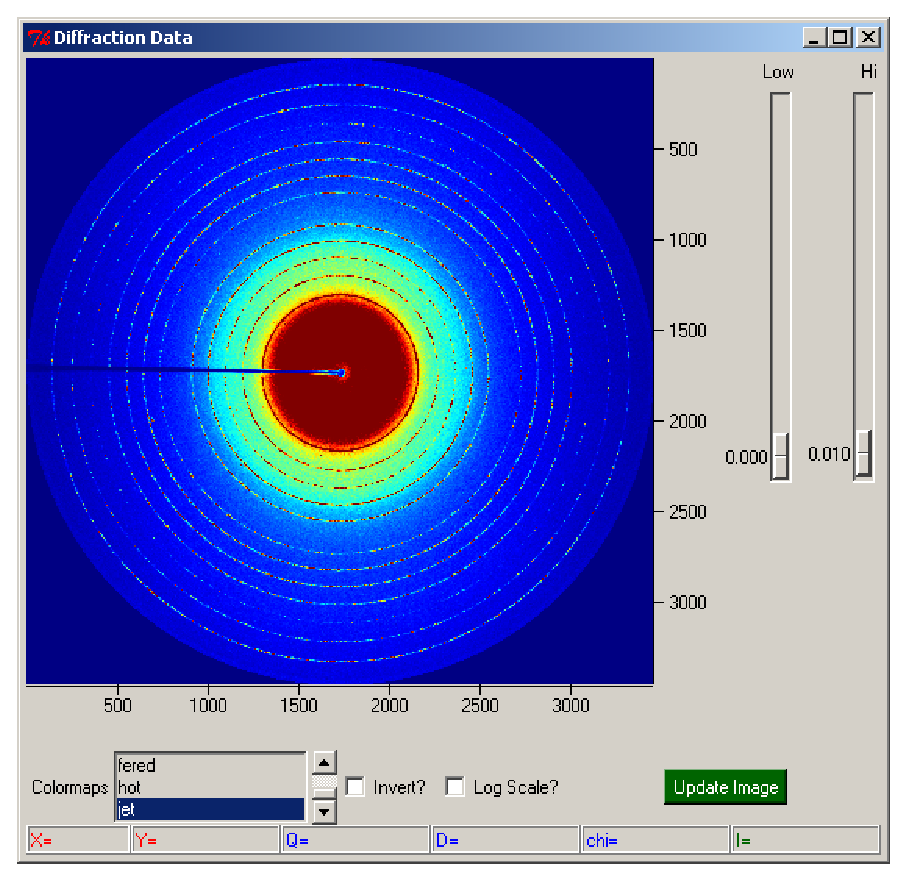
\includegraphics[scale=.5]{figures/diffraction_data_window.eps}\\[1.5cm]

\HRule \\[0.4cm]
{\Huge\rm\bfseries The Area Diffraction Machine}\\[0.1cm]
\HRule \\[1.5cm]

{\Huge\rm \textsc{A Program for Analysis of Two\\
Dimensional Powder Diffraction \\[.4cm]
Data}}\\[1.5cm]
%{\textsc\Huge\rm A Program the Analysis of Two Dimensional Powder Diffraction Data}\\[1.5cm]

{\Large\rm \href{http://areadiffractionmachine.googlecode.com}{areadiffractionmachine.googlecode.com}}


\vfill

{\large \emph{By} Joshua \textsc{Lande} (\href{mailto:joshualande@gmail.com}{joshualande@gmail.com})}\\[.1cm]

{\large \today}

\end{center}

\end{titlepage}




\tableofcontents

\chapter{Tips and Tricks}

\section{Calibration}

The \gui{Calibration} tab can also be used to load
diffraction data into the program. The tab can
be used to calibrate diffraction data to determine the 
parameters that characterize the experiment. 
Diffraction data can be loaded using the \gui{Data File:} input. 
The program recognizes \macroline{mar2300}, \macroline{mar3450}, 
\index{Mar2300}\index{Mar3450}\index{MarCCD}\index{Tiff}
\macroline{mccd}, \macroline{tiff}, and \macroline{edf} data. 
Multiple files can be loaded into the program at the same
time using the file selector and the sum image is loaded.

This program characterizes a diffraction experiment 
according to the parameters:
\index{Calibration Parameters}
\index{X Center}\index{Y Center}
\index{Detector Distance}\index{$\alpha$}
\index{$\beta$}\index{Rotation}\index{Pixel Scale}
\begin{itemize}
    \item \gui{xc:}, \gui{yc:} - the $(x,y)$ pixel coordinate 
    on the detector where the incoming 
    x-ray beam would have hit the detector were there 
    no sample in the way (in pixels).
    \item \gui{d:} -- the distance from the sample to 
    the detector (in mm).
    \item \gui{E:} -- the energy of the incoming beam (in eV).
    \item \gui{alpha:}, \gui{beta:} \gui{R} -- 3 rotations of 
    the detector (in degrees).
    \item \gui{pl:} -- the pixel length of the detector - 
    the width of one pixel (in microns).
    \item \gui{ph:} -- The pixel height of the detector -
    the height of one pixel (in microns).
\end{itemize}
Before calibrating an image, three things must be done. 
First, the diffraction data must be loaded.
Second, a $Q$ data file with standard $Q$ values for the
sample must be loaded.
Third, an initial guess of the calibration parameters must be
loaded. A guess at the calibration parameters can sometimes
be found in the header of the diffraction file. These values
can be loaded into the program using the \gui{Get From Header} 
button.  The \gui{Do Fit} button will perform the calibration 
and find a best guess at the real experimental parameters.

The \gui{Work in Lambda} option in the \gui{Calibration} menu can
be used to make the program work with the x-ray's
wavelength instead of its energy. The calibration parameter 
\gui{$\lambda$:} will be used instead of \gui{E:}.

The \gui{Q Data:} input will load into the program standard $Q$ data files. 
This program stores several standard $Q$ files that can be selected
through the \gui{Standard Q} option of the \gui{Calibration} menu.

The calibration algorithm can be modified in a couple of ways.
The program finds peaks in the diffraction data by 
running from the center of the image out. 
The number of radial slices that the program uses
can be set with the \gui{Number of Chi?} input.
The \gui{Stddev?} input 
tells the program what ratio higher a peak must be than the 
standard deviation of the background near it for the
peak to be considered real. The higher the value, the more
picky the program is about finding legitimate peaks.

If some of the experimental parameters are known exactly, 
the \gui{Fixed?} check box associated with that variable 
will stop it from being refined when fitting. The pixel 
length and pixel height are never refined. 

To see how good the current calibration parameters are, 
the \gui{Draw Q Lines?} 
check box will make the program draw 
on the diffraction image lines of constant $Q$ specified
by the $Q$ data file. The $\Delta Q$ ranges specified in 
the $Q$ data file can be drawn using the \gui{Draw dQ Lines?} 
check box. The diffraction peaks that were found while
calibrating can be displayed using the \gui{Draw Peaks?} check box. 

The diffraction image can be zoomed into by left clicking
on the image, dragging the mouse, and then releasing.
The image can be unzoomed by right clicking on the image. 
The image can be panned across by shift clicking on the image 
and dragging. The image can be made bigger or smaller by 
resizing the window.

In the \gui{File} menu, the \gui{Save Image} option can be used 
to save the current diffraction file in several popular
image formats. The image will be saved with the current
zoom level and any $Q$ lines, $\Delta Q$ lines, peaks, or
masks drawn on it.

\section{Masking}
\index{Pixel Masking}

The program can ignore certain pixels in an image
when performing diffraction analysis. This can be done
using the \gui{Masking} tab.  Threshold masking can be 
used to ignore pixels above or below a certain value.
All pixels larger than a certain value can be masked 
using the \gui{Do Greater Than Mask?} check box
and specifying the value in the 
\gui{(Pixels Can't Be) Greater Than Mask:} input.
All pixels less than a certain value can be ignored 
using the \gui{Do Less Than Mask?} check box 
and specifying the value in the 
\gui{(Pixels Can't Be) Less Than Mask:} input.
The overloaded or underloaded pixels will show up
as a different color on the diffraction and cake images.
This color can be changed using the \gui{Color} buttons
near the other inputs.
When a threshold mask is applied, masked pixels
will not be used during an intensity integration.

The program can mask areas of the diffraction image
using polygon masks. The \gui{Do Polygon Mask?} check box 
will enable this. Any masks in the program
will be displayed over the diffraction data and cake images.
Any masked pixels will not be used during an intensity
integration. The \gui{Add Polygon} button can be used to 
draw new polygon masks. To draw a mask, simply push
the button, left click all the
nodes on the diffraction image except the last one, and
then right click the final node. 
The \gui{Remove Polygon} button can be used to 
remove polygons from the diffraction image. Simply push
the button and then click on the polygon that should be
removed. The \gui{Clear Mask} button will remove all
the polygons from the program. The \gui{Save Mask} button
and the \gui{Load Mask} button will save and load
polygons to and from a file.

\section{Caking}
\index{$\chi$}\index{$Q$}\index{Caking}

A cake is a plot of diffraction data in $Q$ vs.
$\chi$ space. $\chi$ is a measure of the angle around 
the incoming x-ray beam. By convention, $\chi$ is equal to 
$0\degrees$ to the right of the center of the image and
increases in a counterclockwise direction. 
The program needs to know a range and bin size in $Q$ and
$\chi$ in order to make a caked plot. The \gui{Do Cake} button
will create a cake and open a new window with the caked data in
it. The caked window can be interacted with just like
the diffraction window. There is a button called \gui{AutoCake} that 
picks a cake range with the whole diffraction image in it 
and then cakes the data. Any $Q$ lines, $\Delta Q$ lines,
and peaks that are drawn on the diffraction image
will also be drawn on the caked image.
The \gui{Save Data} button will save the caked data
to a file as plain text. The \gui{Save Image} button will save the
caked plot as a popular image format with
any $Q$ lines or peaks that are drawn on 
the caked plot saved on top of it.

The \gui{Do Polarization Correction?} button will apply a 
polarization correction to the caked plot. The polarization
of the incoming beam can be specified with the 
\gui{P?} input. The formula for calculating the 
polarization correction is
\begin{eqnarray}
    I&=&Im/PF \\ 
    PF&=&P(1 - (\sin(2\theta)\sin(\chi-90))^2) + 
    (1 - P)(1 - (\sin(2\theta)\cos(\chi-90))^2)
\end{eqnarray}
with $Im$ the measured intensity. 


\section{Integrate}
\index{Intensity Integration}

An intensity integration is a plot of average intensity
vs. $Q$, $\chi$, or $2\theta$. By default, the options 
available are to integrate in $Q$ or $\chi$. The 
\gui{Work in 2theta} option in the menu bar can be used 
to make the program integrate in $2\theta$ instead of $Q$.  
The program needs to know a range (both a lower and upper value)
and a bin size in order to perform an intensity integration.
When these values have been loaded, the \gui{Integrate} button will 
perform the integration. A new window will open with a plot of data.
By default, the integration will be over all 
possible values of the other variable. This can be changed using the
constraint check boxes. 
For example, selecting the \gui{Constraint With Range on Right?}
check box and setting the \gui{Chi Lower?} input to 0 and the
\gui{Chi Upper?} into to 90 will cause the integration in $Q$
to be only of pixel's with $\chi$ between 0 and 90. 

A polarization correction can be applied during
an intensity integration. The \gui{Save Data} button can be used
to save the intensity data to a file as two column ASCII. 

\section{Macro}\index{Macros}

Macros can be used to speed up data analysis. 
The \gui{Start Record Macro} option in the \gui{Macro} menu
will make the program start recording a macro. After the desired
tasks have been recorded, the \gui{Stop Record Macro} option will
stop the recording and save the commands to a file. The
\gui{Run Saved Macro} option will run a macro file.

Small edits to a macro file can make them much more versatile. 
Most macro commands are just the name of the GUI item
possibly followed by whatever the GUI would want (such as a 
filename or a number). The macro command to load a diffraction 
file is \macroline{Data File:} followed by a line with 
a filename. It can also be followed by a list of filenames,
a directory containing diffraction data, or some combination
of each. The program will run the subsequent macro on
every file in the list and all diffraction files 
in folders in the list. The loop will end with a subsequent 
\macroline{Data File:} line, a \macroline{END LOOP} line, or 
the end of the macro file.

When looping over diffraction files, there is special 
markup which makes it easy to save files in a loop with 
useful names. Whenever the
program finds \macroline{BASENAME} in a macro file,
it will be replaced with the path of the current
diffraction file that has been loaded. Similarly, 
\macroline{FILENAME} will be replaced with the filename of
the current diffraction file. A
diffraction file with the extension \macroline{.mar3450} could be 
recreate with the command \macroline{PATHNAME/FILENAME.mar3450}.
An example of the use of this would be the macro line 
\macroline{Save Integration Data} followed by the line
\macroline{PATHNAME/FILENAME\_int.dat}. The program would always
save the intensity integrated data right next to the diffraction 
file with the same filename but ending with \macroline{\_int.dat}.


\chapter{An Example}
This section will present a pedagogically interesting 
example which demonstrates several of the programs important
features.  The purpose of this chapter is neither to be 
comprehensive nor to be particularly detailed. It will instead 
give a sense of the type of analysis that can be done with 
this program. It will motivate the rest of the manual. further details 
and information on any of the things described below can be found in 
the appropriate sections of the manual.

David, a user of the program, was studying iron thin films 
using powder diffraction. He was particularly interested in 
measuring the shifts in diffraction peaks of a sample. To 
realize this experimentally, he capture the image of the 
standard calibration crystal Lanthanum Hexaboride (LaB6). 
Without changing the experimental parameters, he then imaged 
many samples for which he wanted to measure the shift.

The steps that are needed to do this analysis will be
described. First, we will calibrate the diffraction detector.
This is to say that we want to determine the precise 
experimental parameters that characterized the diffraction
machine when the images were captured (for example, the distance
between sample and detector, the energy of the x-rays, etc). Since 
the image of the standard calibration crystal was taken at the same
time as the images of interest, the calibration parameters inferred
from the standard crystal can be used to analyze the
rest of data.

\begin{SCfigure}[1][hbtp]
    \centering
    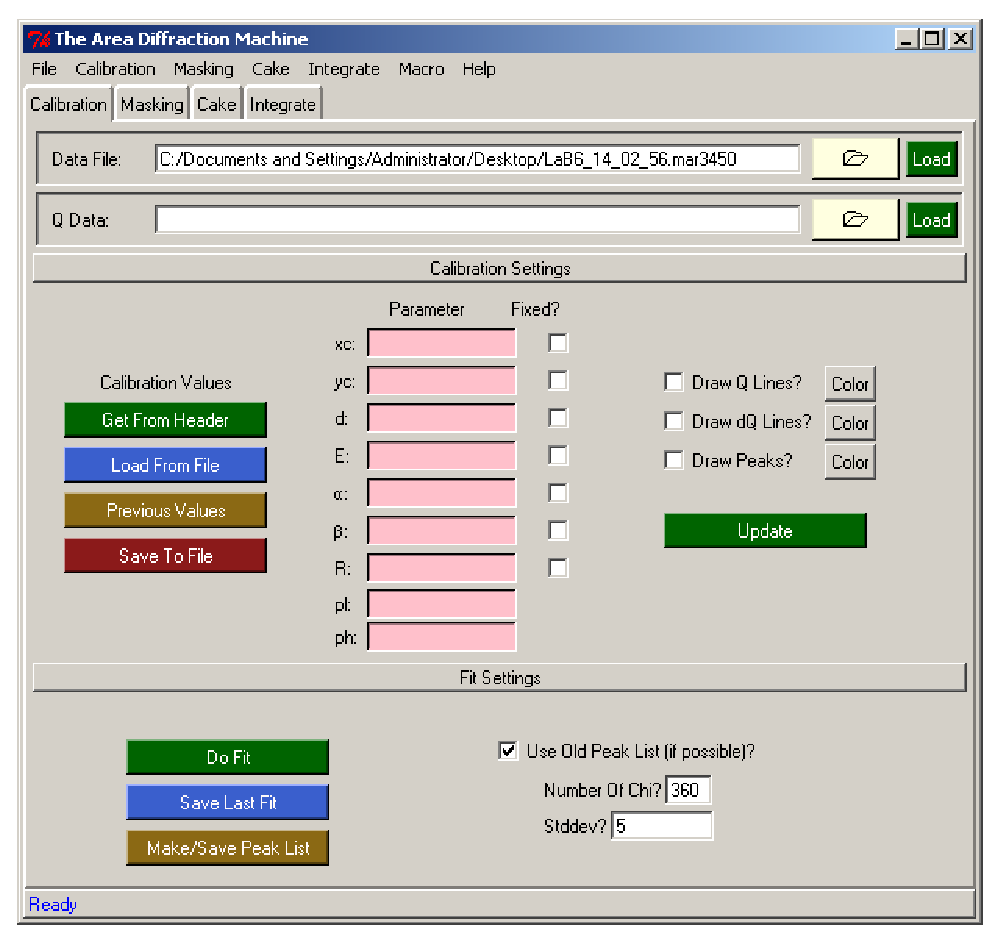
\includegraphics[scale=.75]{figures/calibration_tab.eps}
    \caption{The calibration tab.}
    \label{calibration_tab_example}
\end{SCfigure}

To perform this calibration, we first opened up the Area 
Diffraction Machine. Figure~\ref{calibration_tab_example} shows what we
are first presented with.

From the \gui{Data File} input, we load into the program the LaB6 
file. Once the file is loaded in, a new window opens up 
which shows the diffraction data. This window is shown in 
figure~\ref{diffraction_data_window_example}.

\begin{SCfigure}[1][hbtp]
    \centering
    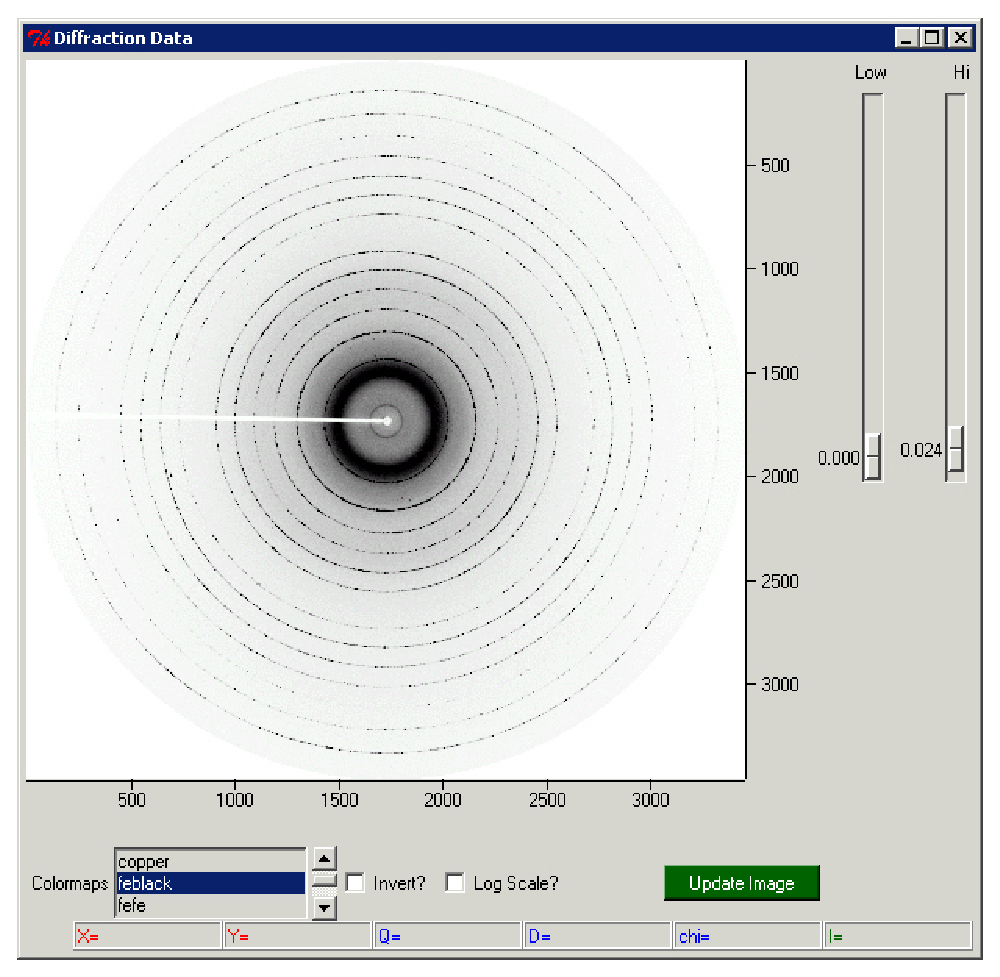
\includegraphics[scale=.75]{figures/diffraction_data_window_example.eps}
    \caption{The diffraction data window.}
    \label{diffraction_data_window_example}
\end{SCfigure}

To do the detector calibration, the program must know the 
$Q$ values associated 
with the standard crystal. Since LaB6 is so common, it is
a preset default in the program. We go into the menu bar, 
into the \gui{calibration} menu, into the \gui{Standard Q} menu, 
and then selected Lanthanum Hexaboride. This is shown
in figure~\ref{standard_q_example}.

\begin{SCfigure}[1][hbtp]
    \centering
    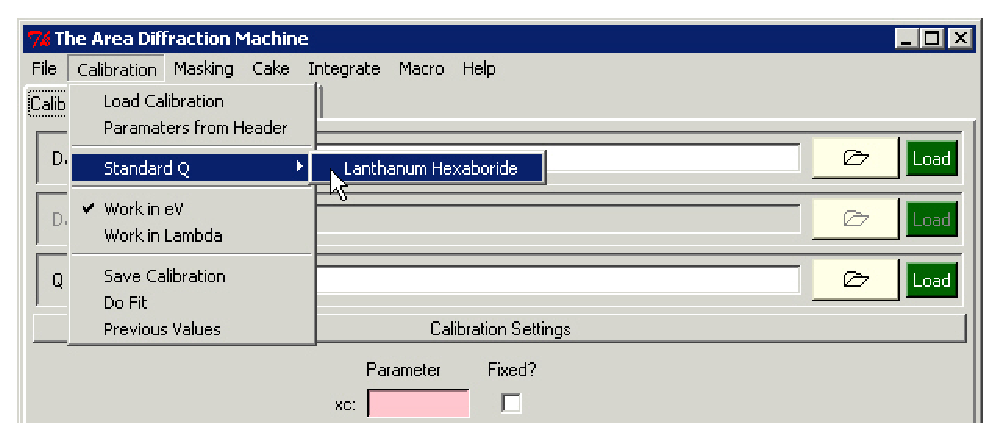
\includegraphics[scale=.75]{figures/standard_q.eps}
    \caption{Loading a standard $Q$ file.}
    \label{standard_q_example}
\end{SCfigure}

(More standard $Q$ files might be added in the future).
In order to perform image calibration, the program finally 
needs to know an initial guess at the calibration parameters. 
Although one could enter these parameters by hand, often 
times decent guesses at the experimental parameters are 
stored in the header data inside of the diffraction image. 
The program can try to find these header calibration values 
and put them into the inputs in the program. To do this, 
we could pushed the \gui{Get From Header} button. With the 
image, the $Q$ values, and an initial guess in the program, 
we are ready to do the calibration. 

But first, we want to examine how good the initial guess 
is. To do so, we can select the \gui{Draw Q Lines?}
check box on the Calibration tab. When this is selected, 
the program will draw
on top of the diffraction image red lines corresponding
to what diffraction pattern should show up on the
detector (for the given calibration parameters and $Q$
values). Figure~\ref{bad_calibration_diffraction_image}
shows what the program displays for our example.

\begin{SCfigure}[1][hbtp]
    \centering
    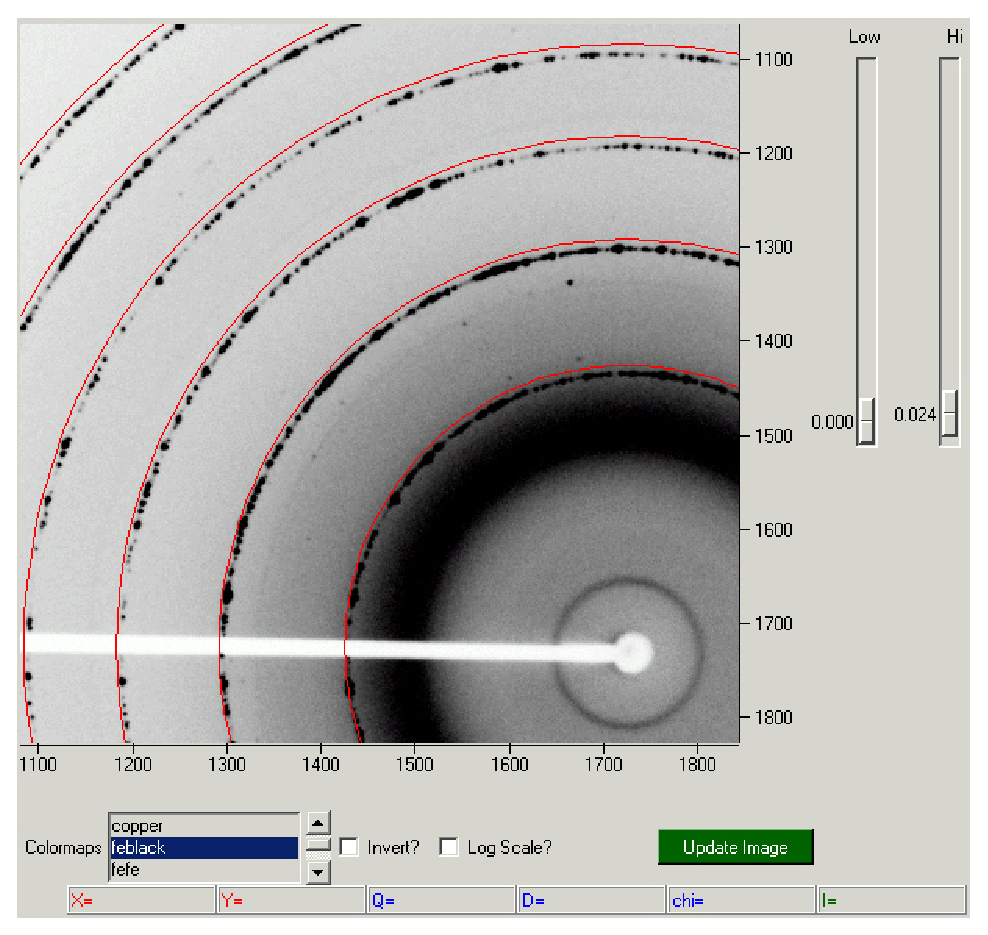
\includegraphics[scale=.75]{figures/bad_calibration_diffraction_image.eps}
    \caption{The diffraction image with constant the $Q$
    lines displayed upon it. These lines are calculated
    for the calibraiton parametesr found in the
    header of the image. They are not particuarly
    accurate.}
    \label{bad_calibration_diffraction_image}
\end{SCfigure}

Of course, our initial guess isn't
great so the red lines don't match too well with
the loaded patter. The data will look like

We can do a cake of the data. A caked plot
is a presentation of the data in a different parameter 
space.  The $x$ axis is $Q$ and the $y$ axis is $\chi$. 
Ideally, if the calibration parameters are known exactly, 
the caked data will show up as many vertical lines. 
We can cake the data by going to the cake tab. This
tab is shown in figure~\ref{cake_tab_example}.

\begin{SCfigure}[1][hbtp]
    \centering
    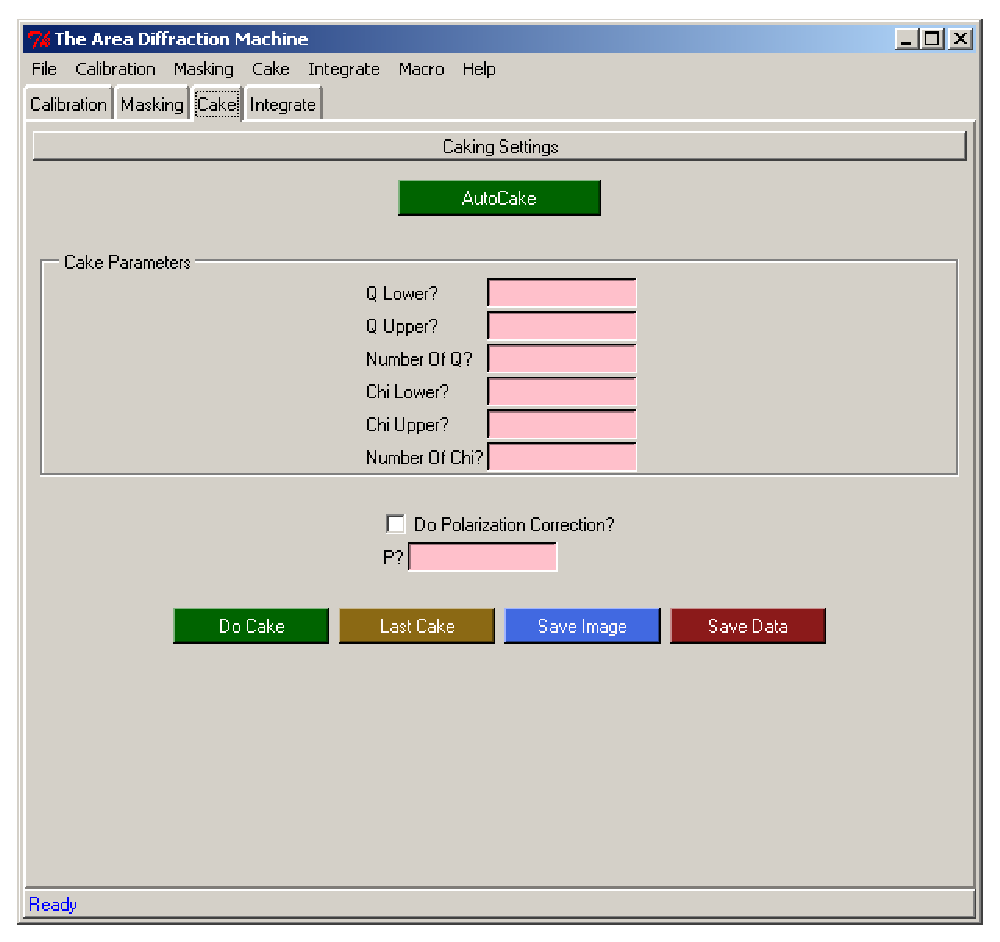
\includegraphics[scale=.75]{figures/caking_tab.eps}
    \caption{The calibration tab.}
    \label{cake_tab_example}
\end{SCfigure}

On this tab, we have to pushing the \gui{AutoCake}. 
When we do so, a new cake window opens up. 
Figure~\ref{bad_calibration_cake} shows what the 
program displays for our example.

\begin{SCfigure}[1][hbtp]
    \centering
    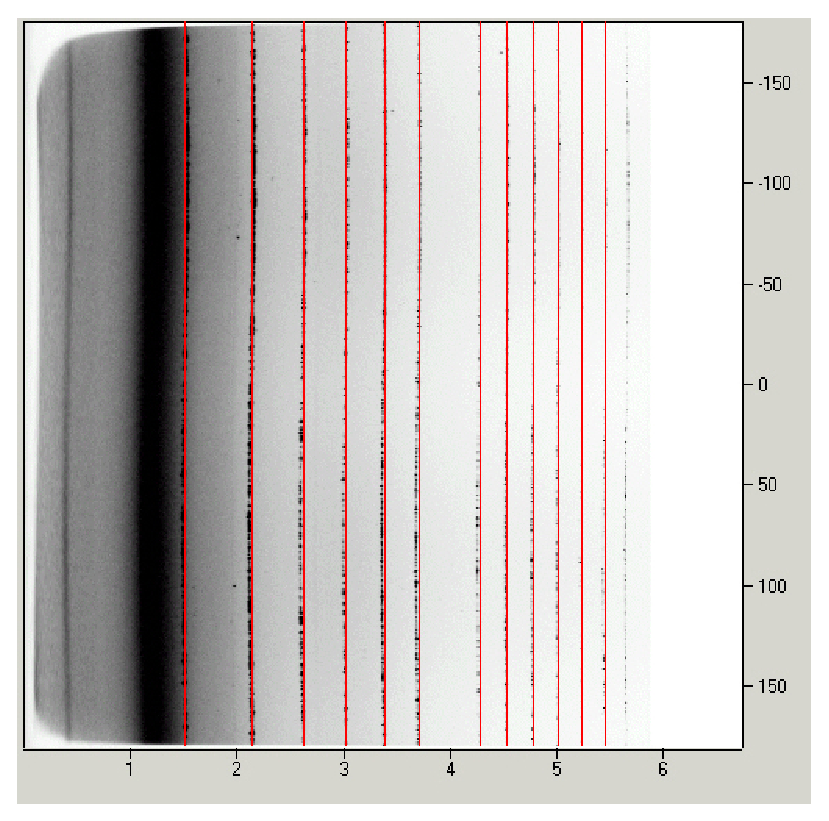
\includegraphics[scale=.75]{figures/bad_calibration_cake.eps}
    \caption{A caked plot done with the calibration parameters
    found in the header of the image. The header parameters
    are not particuarly obvious and the diffraciton peaks
    are not particuarly straight. Calibratin helps improve
    the strightness of the diffraciton peaks.}
    \label{bad_calibration_cake}
\end{SCfigure}

We see that for The caked data with the initial guess 
calibration parameters, our diffraction lines
have a systematic wiggle. It might be hard to see 
with the full image, but by zooming into just one
line we find the difference to be much more obvious.
A zoomed in range is shown in 
figure~\ref{bad_calibration_cake_zoom}.

\begin{SCfigure}[1][hbtp]
    \centering
    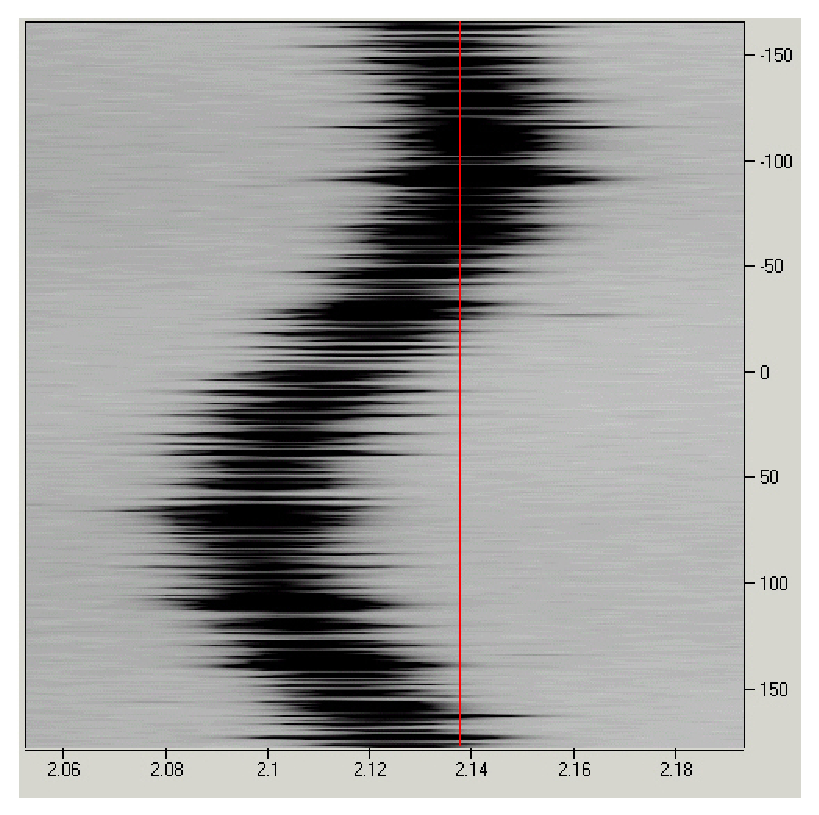
\includegraphics[scale=.75]{figures/bad_calibration_cake_zoom.eps}
    \caption{A zoom in of the cake shown in 
    figure~\ref{bad_calibration_cake}. When zoomed into 
    diffraction image, the poor calibration becomes much 
    more obvious.}
    \label{bad_calibration_cake_zoom}
\end{SCfigure}

This means that our initial guess at 
calibration parameters is not great.
We can now do the calibration. To do so, we push
the \gui{Do Fit} button on the \gui{Calibration}
tab. If the calibraiton did a good job, the constant
$Q$ lines drawn on the diffraction image move
so that they are entirely over the diffraction 
pattern. This is shown in 
figure~\ref{good_calibration_diffraction_image}.

\begin{SCfigure}[1][hbtp]
    \centering
    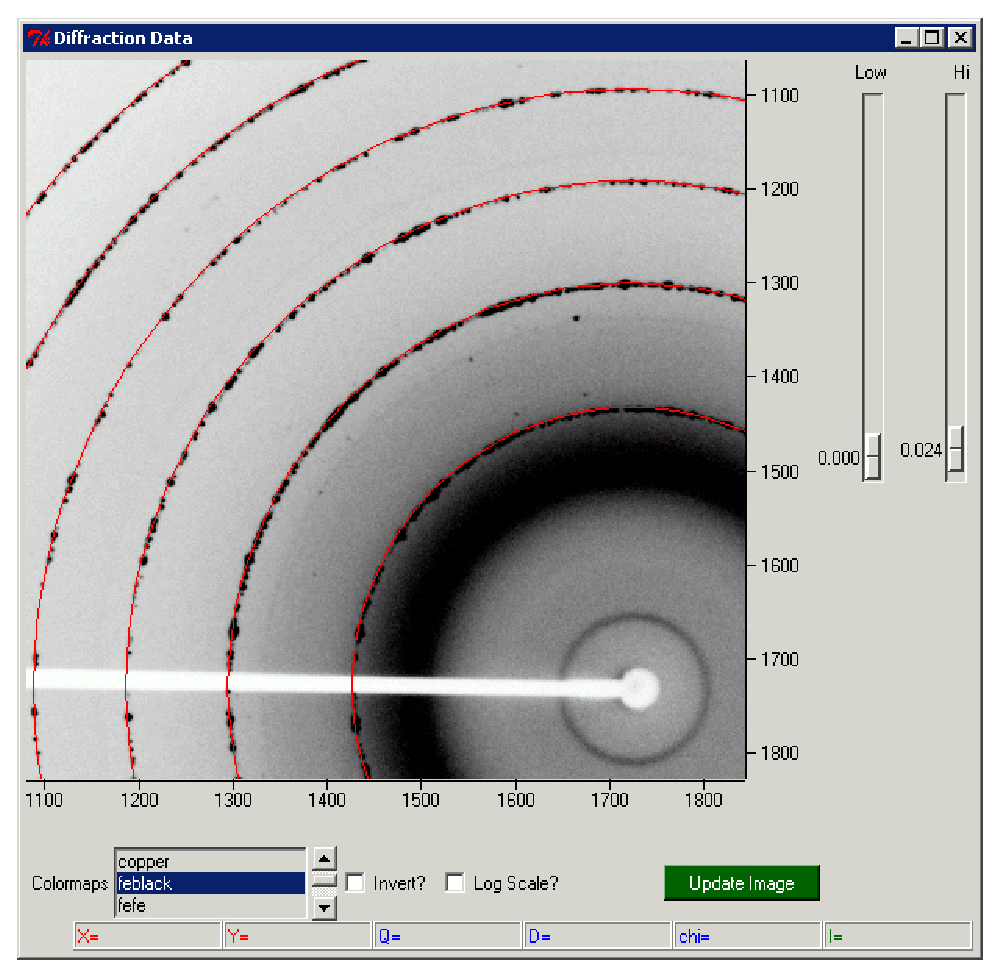
\includegraphics[scale=.75]{figures/good_calibration_diffraction_image.eps}
    \caption{The diffraction window after being calibrated. The
    constant $Q$ lines fall well on top of the diffraction 
    peaks.}
    \label{good_calibration_diffraction_image}
\end{SCfigure}

The diffraction peaks on the caked image become much straigher.
The caked window after calibraiton is shown in 
figure~\ref{good_calibration_cake}.

\begin{SCfigure}[1][hbtp]
    \centering
    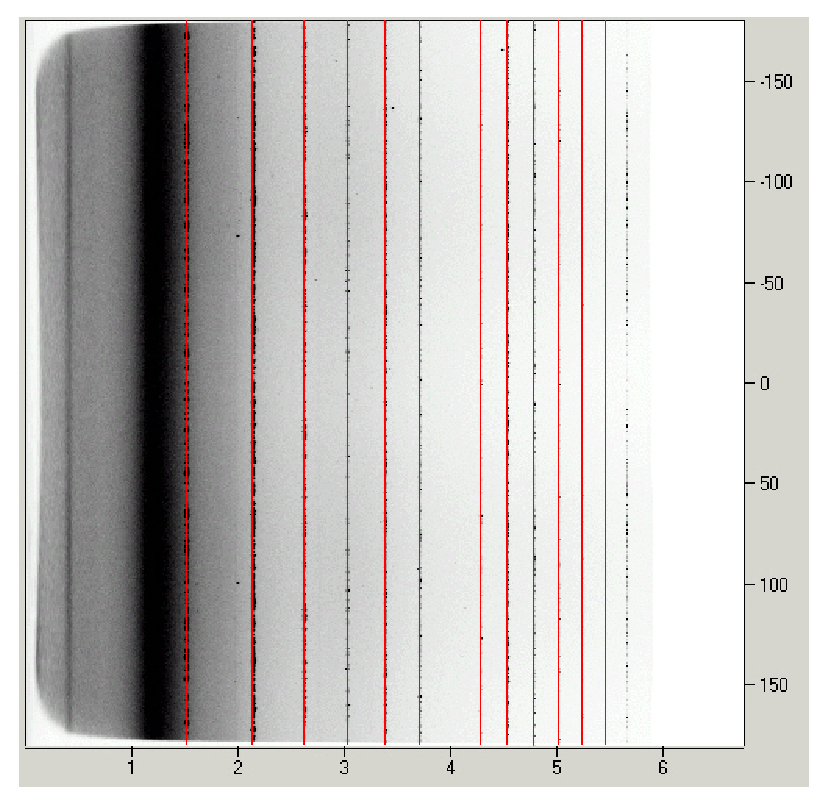
\includegraphics[scale=.75]{figures/good_calibration_cake.eps}
    \caption{The cake window after calibration.  The lines 
    are much straigher then the lines in 
    figure~\ref{bad_calibration_cake} before calibration.}
    \label{good_calibration_cake}
\end{SCfigure}

They look good even when zoomed in. A corresponding zoom in of
the caked window in shown in 
figure~\ref{good_calibration_cake_zoom}.

\begin{SCfigure}[1][hbtp]
    \centering
    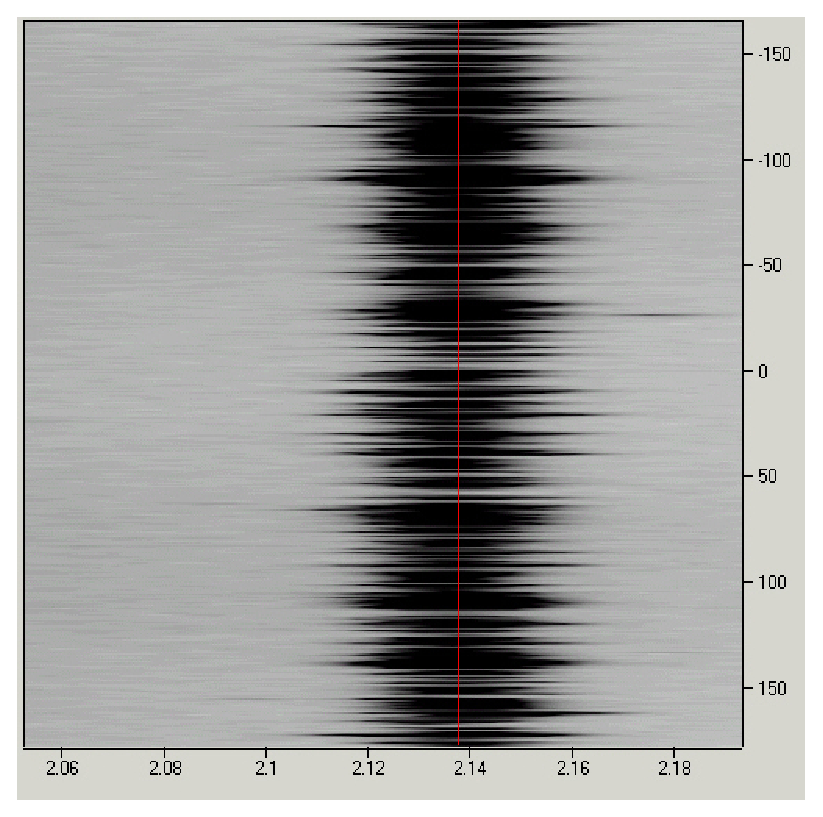
\includegraphics[scale=.75]{figures/good_calibration_cake_zoom.eps}
    \caption{A zoomed in part of figure~\ref{good_calibration_cake}. 
    Even at a large zoom in, the line remains very straight.}
    \label{good_calibration_cake_zoom}
\end{SCfigure}

After caking the calibrated data and convincing ourselves that
our calibration parameters are good, we can save the calibration
parameters to a file for later use. We can do so using the
\gui{Save to File} button on the \gui{Calibration} tab.
After selecting the location \gui{C:/Data/LaB6\_cal.dat}, the
calibration file gets saved as
\begin{lstlisting}[caption={'The Calibration Parameters File'}]
xc	1722.966078	0
yc	1724.227970	0
D	122.691351	0
E	12707.219316	0
alpha	-0.052910	0
beta	0.130553	0
rotation	-41.523477	0
pixelLength	100.000000
pixelHeight	100.000000
\end{lstlisting}

\begin{SCfigure}[1][hbtp]
    \centering
    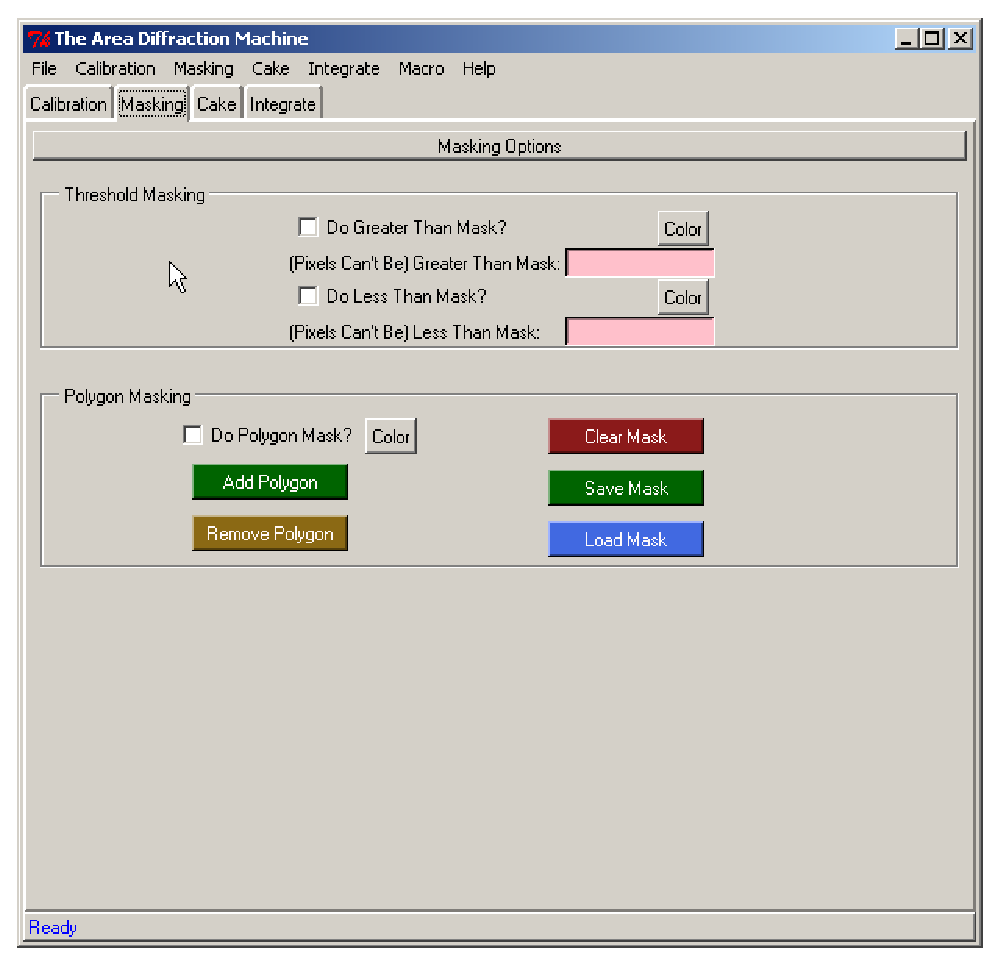
\includegraphics[scale=.75]{figures/masking_tab.eps}
    \caption{The pixel masking tab.}
    \label{masking_tab_example}
\end{SCfigure}

As can be seen in figure~\ref{diffraction_data_window_example},
there is a beam stop on the left side of the image which is
obstrucing part of the image. We know that none of the pixels
blocked by the beam stop contain any interesting information
so we are going to want to tell the program to ignore any pixels
blocked by the mask. We can do so with a polygon mask. All
polygon masking is done on the \gui{masking} tab. A screenshot
of this tab is shown in figure~\ref{masking_tab_example}.
We want to add a rectangular polygon mask on top of the beam
stop in the image. To do so, we push the \gui{Add Mask} button.
We then move to the diffraction image and draw the beamstop
on the image by left clicking nodes on the screen. We add the
final node by right clicking. After having drawn the polygon mask, 
our diffraction image is shown in figure~\ref{masked_beam_stop}.

\begin{SCfigure}[1][hbtp]
    \centering
    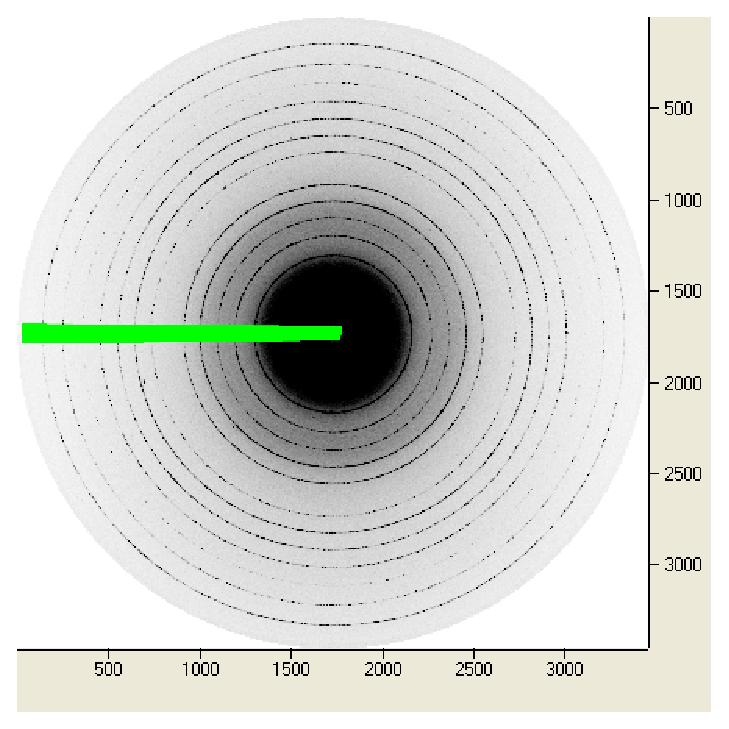
\includegraphics[scale=.75]{figures/masked_beam_stop.eps}
    \caption{Here is the same diffraction data as in 
    figure~\ref{diffraction_data_window_example} but with a
    polygon mask drawn over the beam stop. This polygon mask
    will stop the beam stop below it from being used in
    subsequent data analysis.}
    \label{masked_beam_stop}
\end{SCfigure}

Once we decide we are happy with our polygon mask, we can
save it to a file using the \gui{Save Mask} button.
The file gets saved out as
\begin{lstlisting}[caption={'beam\_stop\_mask.dat'}]
# Polygon(s) drawn on Mon Apr 14 00:33:12 2008
25.6749379653	1634.63771712
42.7915632754	1814.36228288
1959.85359801	1857.15384615
1959.85359801	1626.07940447
\end{lstlisting}
We can then load in this mask when we do the rest of
our analysis. The mask will make sure that none of the
the pixels within the beam stop are used for any subsequent
analysis.

Now, we are going to want to perform an intensity integration 
of the rest of our data. We can use the intensity
integrate data to look for peaks in the data.
The steps for doing the rest of
this analysis are as follows. Load in particular file we
are interested in. Load in these calibration parameters
using the \gui{Load From File} button on the \gui{Calibration}
tab.\footnote{If you just did the calibration, the 
parameters should already be in the inputs. The point is
just that you could load the parameters into the program
if you were, say, to open the program at some later point
in time.}. Next, we can load in our previously recorded
beam stop mask using the \gui{Load Mask} button on the
\gui{Masking} tab. We also have to make sure polygon masks
are used in the analysis by making sure the 
\gui{Do Polygon Mask?} check box is selected.
With everything loaded into the program, 
we can perform a $Q$ integration by going to the 
\gui{Integrate} tab. The integration tab is shown in 
figure~\ref{integration_tab_example}

\begin{SCfigure}[1][hbtp]
    \centering
    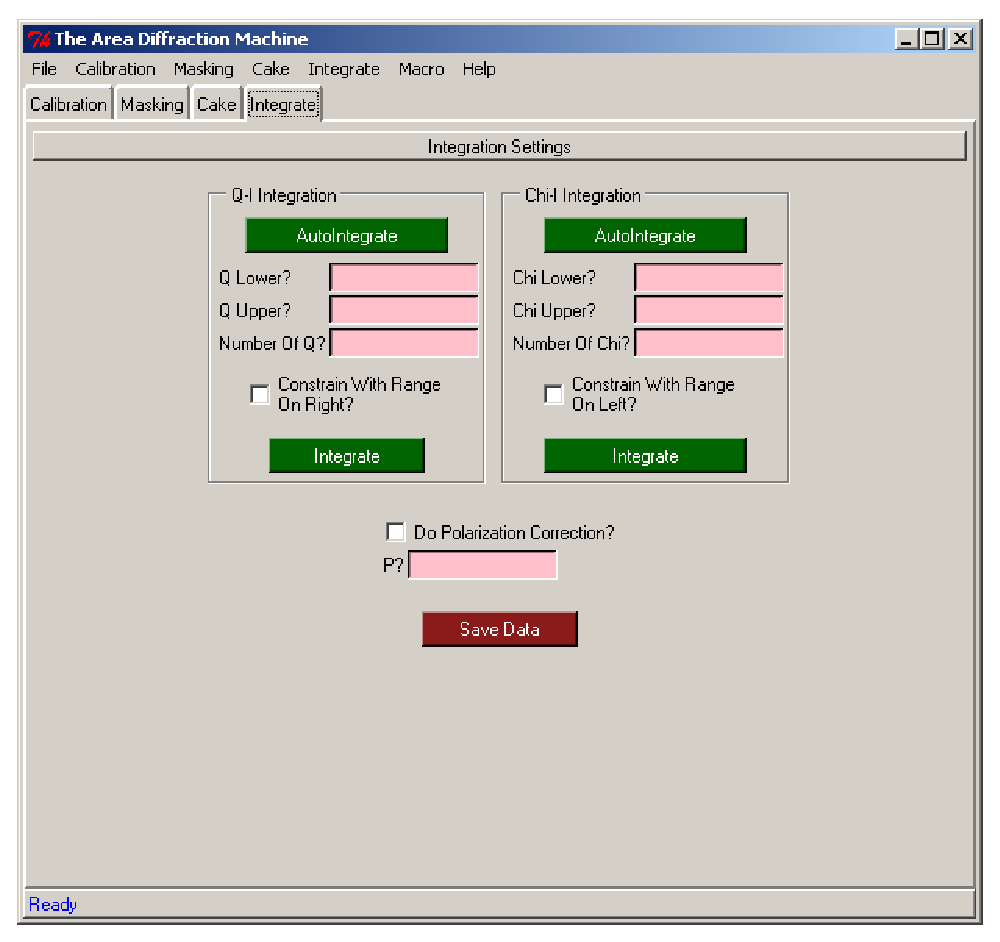
\includegraphics[scale=.75]{figures/integration_tab.eps}
    \caption{The integration tab.}
    \label{integration_tab_example}
\end{SCfigure}

We set the range of the $Q$ integration by setting
\gui{Q Lower?} to 0 and \gui{Q Upper?} to 5. We
then set the precision of the integration, or the
bin size, by setting the \gui{Number of Q?} input
to 300. Finally, we push the left \gui{Integrate}
button and a window showing the diffraction data
opens. For a particular iron sample, this window
is shown in figure~\ref{iron_intensity}.

\begin{SCfigure}[1][hbtp]
    \centering
    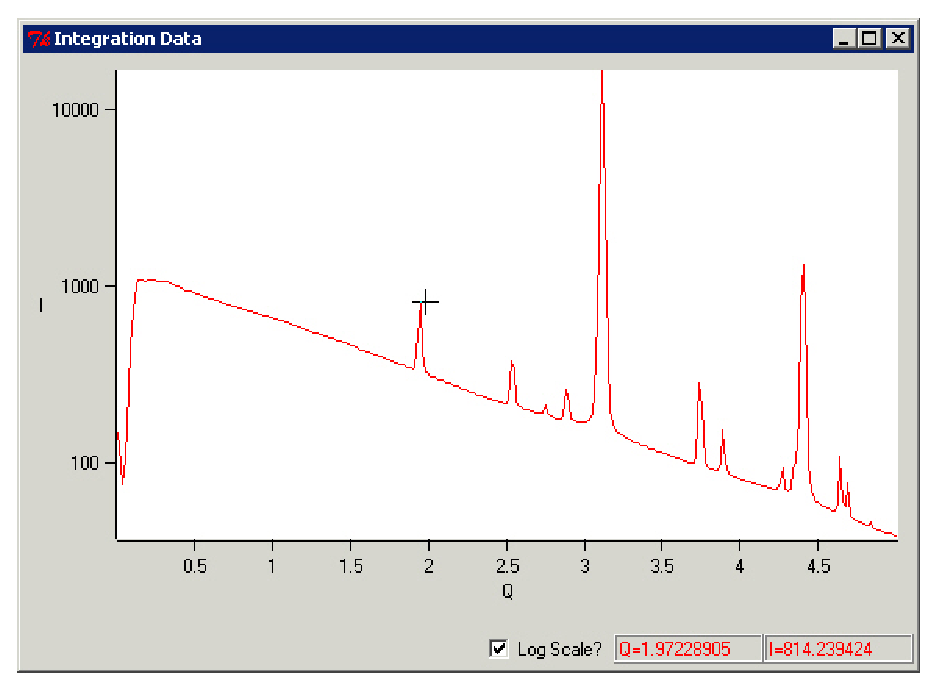
\includegraphics[scale=.75]{figures/iron_intensity.eps}
    \caption{The intensity integration window for 
    a particular iron sample.}
    \label{iron_intensity}
\end{SCfigure}

We can save this data to a file with the \gui{Save Data}
button on the \gui{Integration} tab. This data is
saved out as two column ASCII.
After doing this for all the different files that
we have, we can load all the data into another program,
such as Microsoft Excel, and compare the peaks.

But if there are a lot of files to analyze, this whole
process can be very time consuming. Instead of doing 
this analysis by hand, we can automate the process by
writing a macro to analyze all the files one at a 
time. First, we put all of our data into \macroline{C:/Data/}.
The macro that we can run is
\begin{lstlisting}[caption={'A macro to automate the 
    analysis'}]
Data File:
	C:/Data/
Load From File
    C:/Data/LaB6_cal.dat
Load Mask
    C:/Data/beam_stop_mask.dat
Do Polygon Mask?
    Select
Integrate Q Lower?
	0
Integrate Q Upper?
	5
Integrate Number of Q?
	300
Integrate Q-I
Save Integration Data
    PATHNAME/FILENAME_int.dat
\end{lstlisting}
The first command loads into the program all of the
diffraction files in the folder \macroline{C:/Data/}
one at a time and runs the rest of the analysis on
that particular file. The program then loads in
the calibration file that we saved earlier and sets the
integration bounds. Then the progarm loads in the
beam stop mask. Then, the program does a 
$Q$ vs intensity integration and saves the intensity
integrated data to a file. The PATHNAME keyword gets
repalced with teh path leading up to the particular 
file and the FILENAME keyword gets replaced with 
the particular file's name. For example, the file
\macroline{FeL2\_d070.mar3450} in
the folder \macroline{C:/Data/} would
be replaced with
\macroline{C:/Data/FeL2\_d070\_int.dat}
This command will let us save out of our intesnity
integrated data next to the corresponding diffraction
file with a useful filename.

After we run this macro, all of our data will 
be saved out into text files. We can, for
example, open the files in Excel and plot
the different diffraction patterns on the same
graph. If we did this, we would obtain a plot
that looked something like the graph shown
in figure~\ref{excel_peak_shift}.

\begin{SCfigure}[1][hbtp]
    \centering
    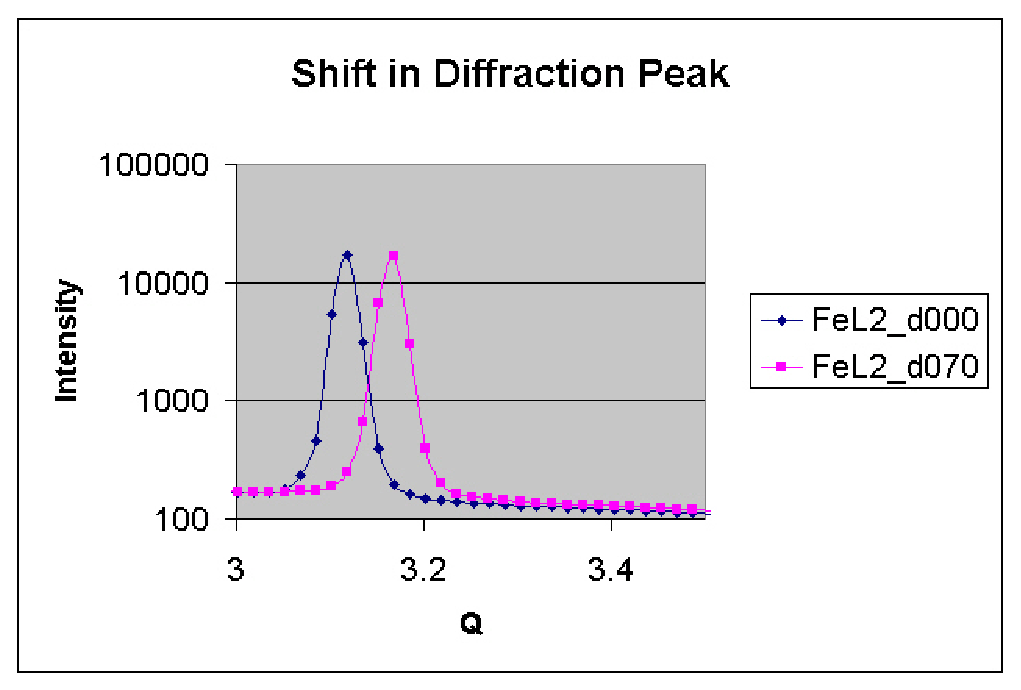
\includegraphics[scale=.5]{figures/excel_peak_shift.eps}
    \caption{An example of what the shift in peaks might
    look like when two diffraction patterns were plotted
    in Excel on top of one another.}
    \label{excel_peak_shift}
\end{SCfigure}




\begin{SCfigure}[1][htb]
    \centering
    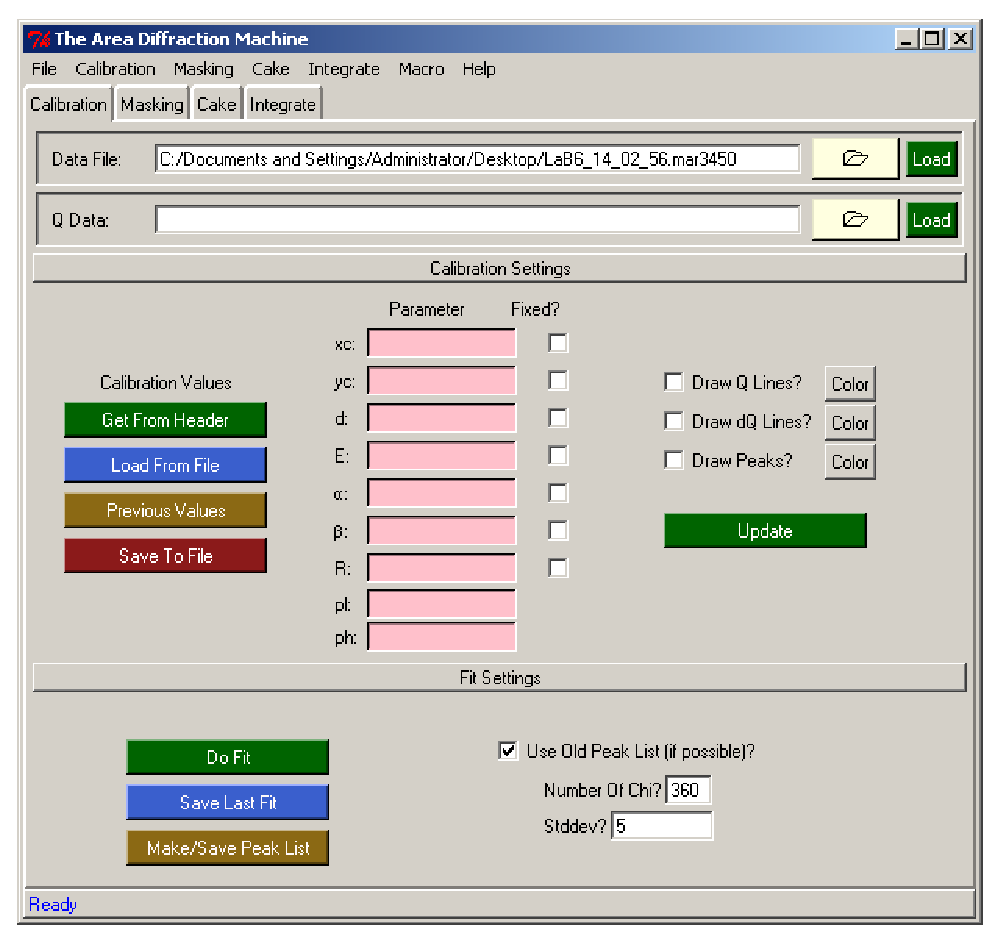
\includegraphics[scale=.75]{figures/calibration_tab.eps}
    \caption{A screen shot of the calibration tab.
    This is what you see when you first open the program. 
    This tab allows you to load diffraction
    data into the program.} 
    \label{calibration_tab}
\end{SCfigure}

When you first opep the Area Diffraction Machine, you
will see the calibration tab. It is shown in 
figure~\ref{calibration_tab}. The first thing you
will probably want to do is load diffraction data into
the program. This can be done with the \gui{Data File:} input
either by typin in the filename by hand and pushing the
load button or clicking on the folder icon and
using a file selector. After the file is loaded, a
diffraction data window will open. This window is 
shown in figure~\ref{diffraction_data_window}.

\begin{SCfigure}[1][htb]
    \centering
    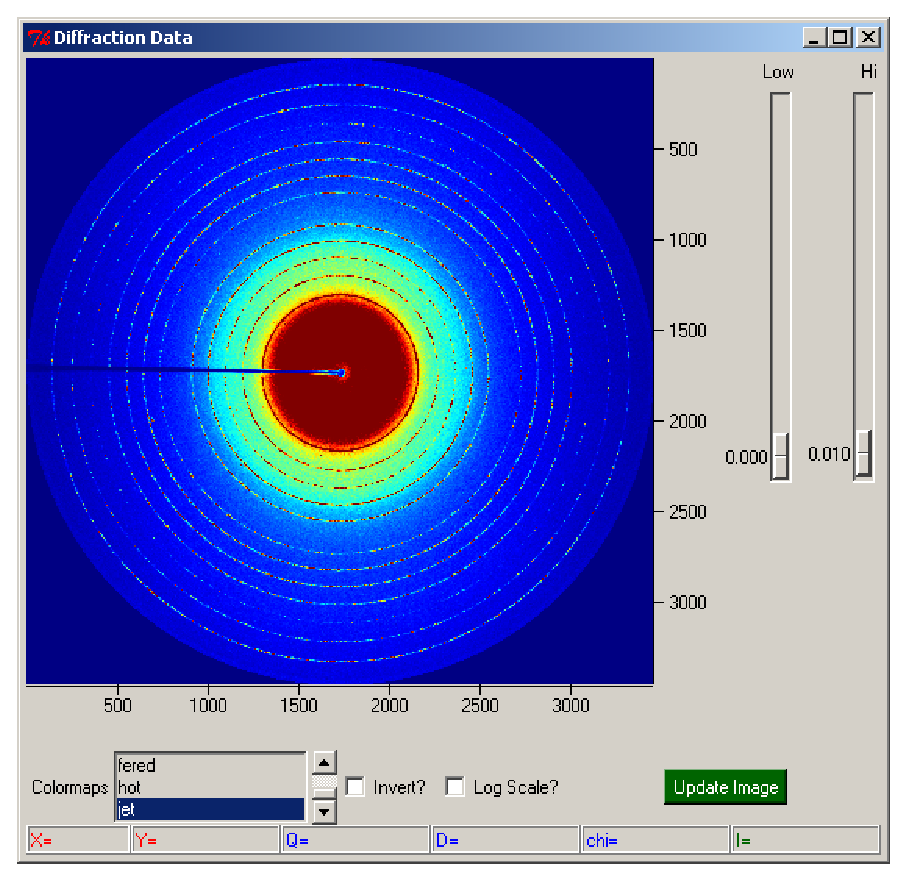
\includegraphics[scale=.75]{figures/diffraction_data_window.eps}
    \caption{A screen shot of the diffraction data window. This 
    window will open after a file is 
    loaded. This windows allows you to interact with diffraction 
    data.} 
    \label{diffraction_data_window}
\end{SCfigure}

You can use the diffraction data window to interact with your 
diffraction data. you can:
\begin{itemize}
    \item {\em Zoom into the data} -- left click on
    the data and hold down on the mouse. When you drag the cursor, 
    the program will create a resizing square. When you let go of the
    mouse, the selected square will be used as the outer bound and
    the image will be zoomed into it.
    \item {\em Zoom out of the data} -- right click on
    the data.
    \item {\em Pan across the data} -- hold shift, push down either mouse
    button, and then move the mouse around and the image will move 
    with it. Let go of the mouse to stop panning.
    \item {\em Resize the window} -- Click on the bottom right corner of
    the window and drag. The window will reszie just like any
    other program.  
    \item {\em Read coordinates for a selected point} -- When you
    mouse over the image, the $x$, $y$, $Q$, $\chi$, and $I$
    values for that pixel will be displayed at the bottom of the
    window. $Q$ and $\chi$ will only be dipslayed if valid calibration
    data is loaded into the program. See chapter~\ref{calibration}.
    \item {\em Change the Color Map} -- The \gui{Colormaps} selector 
    can be used to change the particular color map used to display the 
    data.
    \item {\em Invert the Color Map} -- The \gui{Invert?} checkbox can 
    can be used to invert the colors of the color map.
    \item {\em Low \& Hi Pixels} -- The sliders to the right of the 
    image can be used to change the intensity scaling of the
    image. The low value corresponds to the intenisty 
    value that will be maped to the lowest part of
    the color map and the hi value corresonds to the intensity
    value that will be mapped to the highest part of the color
    map. \footnote{Technically, what you actually set is what
    percentage of the most intense pixel in the image should be 
    mapped to the lowest or highest value in the color map.}
    This feature is useful because it can help make visible certain
    intensity ranges of the image.
    \item {\em Log Scaling} - By default, intensity values are linearly 
    mapped to colors in the color map. The \gui{Log Scale?} checkbox 
    can be selected to instead apply a log scale mapping of the intensity 
    values to the color map.
\end{itemize}

\section{File Formats}

The program can load in Mar data: \macroline{.mar2300}, 
\macroline{.mar3450}, and the \macroline{.mccd} Mar CCD format.
It can load in standard \macroline{.tiff} data. 
It can load in the ESRF Data Format \macroline{.edf}.
The program can only display square data. Whenever non-square
data is loaded into the program, the program will simply pad 
out the image until it is a square with pixels who's intensity is 0. 

\section{Loading Multiple Images}

Using the same file input, you can load multiple files into 
the program at the same time. If multiple files are put in 
the \gui{Data File:} text input  and separated by spaces, they
will all be loaded in. Alternately, the diffraction data file 
selector can be used to select multiple files at the same time.
All of the selected files will be loaded.
When several files are loaded at the same time, the program will 
add the intensities of the images pixel by pixel and work with the 
combined image.  This can be useful for analyzing several images 
taken of the same sample. The program can only add together files 
of the same format.

\section{Saving the Diffraction Image}
\index{Save}\index{ESRF Data Format}

You can save diffraction data in the program as a popular image format. 
The data can be saved by doing to the \gui{File} menu bar and selecting 
the \gui{Save Image} option.  The formats currently allowed are \gui{jpg}, 
\gui{gif}, \gui{eps}, \gui{pdf}, \gui{bmp}, \gui{png}, \gui{tiff}, and 
the ESRF data format \gui{edf}.

Images saved as a popular image format will be saved with whatever
threshold masks, polygon masks, $Q$ lines, $\Delta Q$ lines, and peaks 
are currently displayed over the data in the diffraction data 
window. And it will be saved at whatever the current zoom level 
is.\footnote{This is not the case with ESRF data. When an image
is saved as an ESRF file, it will be saved un-zoomed with none
of the lines or masks on top of it.} See chapter~\ref{calibration} for 
a discussion of the $Q$ lines, $\Delta Q$ lines, and peaks. See 
chapter~\ref{pixel_masking} for a discussion of threshold masks and 
polygon masks.

Because the program will pad any non-square data when
it is loaded to. The program will always save out 
all images as squares. If this is undesirable, the saved images
will need to be cropped using another program.



\chapter{Detector Geometries}\label{theory_chapter}

X-ray diffraction can be modeled as in figure~\ref{DiffractionSetup}. 
Cones of light preferentially leave a crystal at particular angles to 
the incoming beam. These cones of light are 
captured by a detector. The scattering angle 
of an x-rays is called 
$2\theta$. Usually, the interesting thing to measure by doing x-ray 
diffraction is $2\theta$. If we placed a detector perpendicular 
to the incoming beam, the cones of light would be detected as 
circles of high intensity. 
If we knew the distance $d$ from the sample to the detector and 
the distance $r$ from the center of the detector to a 
particular ring, we could easily calculate the scattering angle 
of the light 
\begin{equation}
    \tan2\theta = \frac{r}{d}.
\end{equation}
This is shown in figure~\ref{MeasureAngleFlatDetector}. 
Life is not always so simple. The detector is never
exactly perpendicular to the incoming beam.  In practice, 
the detector will always be slightly titled with respect 
to the incoming beam. Failing to account for this would
introduce a systematic error in the angle measurements.

\begin{SCfigure}[1][htbp]
    \centering
    % Generated with LaTeXDraw 1.9.5
% Sun Apr 20 22:09:06 EDT 2008
% \usepackage[usenames,dvipsnames]{pstricks}
% \usepackage{epsfig}
% \usepackage{pst-grad} % For gradients
% \usepackage{pst-plot} % For axes
\scalebox{1} % Change this value to rescale the drawing.
{
\begin{pspicture}(0,-2.9240625)(6.22,2.9575)
\psellipse[linewidth=0.04,dimen=outer](4.6,0.1825)(1.0,2.0)
\pspolygon[linewidth=0.04,linecolor=white,fillstyle=solid](3.6,1.3559375)(4.2,1.8159375)(4.1,-1.3840625)(3.52,-0.9640625)
\psline[linewidth=0.04cm](2.0,0.1425)(4.64,2.1625)
\psline[linewidth=0.04cm](2.0,0.1425)(4.62,-1.7975)
\psline[linewidth=0.04cm](2.0,0.1425)(5.6,0.1425)
\psline[linewidth=0.04cm](2.0,0.1425)(5.28,-1.2575)
\psline[linewidth=0.04cm](2.0,0.1425)(5.38,1.3425)
\psline[linewidth=0.04cm](0.0,0.1425)(1.6,0.1425)
\psline[linewidth=0.04](3.4,1.2159375)(3.4,2.8825)(6.2,2.0825)(6.2,-2.9175)(3.4,-1.9175)(3.4,-0.9040625)
\usefont{T1}{ptm}{m}{n}
\rput(5.44,2.7825){Detector}
\usefont{T1}{ptm}{m}{n}
\rput(1.69,0.7825){Crystal}
\pspolygon[linewidth=0.04](1.6,0.3025)(1.6,0.0025)(1.8095238,-0.1975)(2.0,-0.0175)(2.0,0.3025)(1.8,0.5025)
\psline[linewidth=0.04cm,linestyle=dashed,dash=0.16cm 0.16cm](3.4,1.2359375)(3.4,-0.9240625)
\psellipse[linewidth=0.04,linestyle=dashed,dash=0.17638889cm 0.10583334cm,dimen=outer](4.6,0.1825)(1.0,2.0)
\end{pspicture} 
}


    \caption{An X-Ray diffraction setup. X-rays scatter from a 
    3-D sample and are captured by a 2-D detector. In this 
    setup, the detector is perpendicular to the incoming 
    x-ray beam.}
    \label{DiffractionSetup}
\end{SCfigure}

\begin{SCfigure}[1][htbp]
    \centering
    % Generated with LaTeXDraw 1.9.5
% Thu Mar 13 00:25:02 EDT 2008
% \usepackage[usenames,dvipsnames]{pstricks}
% \usepackage{epsfig}
% \usepackage{pst-grad} % For gradients
% \usepackage{pst-plot} % For axes
\scalebox{1} % Change this value to rescale the drawing.
{
\begin{pspicture}(0,-2.92)(6.22,2.92)
\psellipse[linewidth=0.04,dimen=outer](4.6,0.2)(1.0,2.0)
\psline[linewidth=0.04cm](2.0,0.16)(4.64,2.18)
\psline[linewidth=0.04cm](2.0,0.16)(4.62,-1.78)
\psline[linewidth=0.04cm](2.0,0.16)(4.58,0.18)
\psline[linewidth=0.04cm](2.0,0.16)(5.38,1.36)
\psline[linewidth=0.04cm](0.0,0.16)(1.6,0.16)
\psline[linewidth=0.04](3.4,1.7)(3.4,2.9)(6.2,2.1)(6.2,-2.9)(3.4,-1.9)(3.4,-1.3)
\pspolygon[linewidth=0.04](1.6,0.32)(1.6,0.02)(1.8095238,-0.18)(2.0,0.0)(2.0,0.32)(1.8,0.52)
\psline[linewidth=0.04cm](4.56,0.18)(5.38,1.34)
\psline[linewidth=0.04](4.34,0.18)(4.49,0.32)(4.64,0.32)
\psline[linewidth=0.04cm,tbarsize=0.07055555cm 5.0]{|-|}(2.08,-0.22)(4.58,-0.22)
\psline[linewidth=0.04cm,tbarsize=0.07055555cm 5.0]{|-|}(4.9,0.06)(5.7,1.26)
\usefont{T1}{ptm}{m}{n}
\rput(3.2314062,-0.215){\psframebox[linewidth=0.028222222,linecolor=white,fillstyle=solid,framesep=0.0,boxsep=false]{$d$}}
\usefont{T1}{ptm}{m}{n}
\rput(5.2014065,0.585){\psframebox[linewidth=0.02,linecolor=white,fillstyle=solid,framesep=0.02]{$r$}}
\psarc[linewidth=0.04](3.18,0.44){0.38}{315.0}{38.65981}
\usefont{T1}{ptm}{m}{n}
\rput(3.2514062,0.365){$2\theta$}
\pscircle[linewidth=0.04,dimen=outer,fillstyle=solid](5.4,1.36){0.12}
\end{pspicture} 
}


    \caption{The same setup as in figure~\ref{DiffractionSetup}. 
    $2\theta$ is the scattering angle of the light,
    $d$ is the distance 
    from the crystal to the detector, and $r$ is the distance 
    from the center of the detector.}
    \label{MeasureAngleFlatDetector}
\end{SCfigure}

There is a need to analyze diffraction data on detectors that are 
not perpendicular to the incoming x-rays. We will present a 
theory of tilted detectors first developed by Abhik Kumar 
in~\cite{Kumar05}.\index{Abhik Kumar} Our derivation will result in 
different formulas because of different assumptions
about how the detector is tilted. 

What we are interested in relating
coordinates on a tilted detector 
to theoretically motivated quantities such as 
the scattering angles of the beam that hit the
detector. We must first work
out the transformation of points on a tilted detector
to points on an untilted detector a known distance
away. This is to say
that we want to figure out where on an untilted 
detector a beam would have hit were it to hit
the untilted detector instead of the tilted detector.
We will call the point on the untilted detector
as measured on the untilted detector $(x,y)$ 
and the corresponding point on the tilted detector
as measured on the tilted detector as $(x''',y''')$. 
The reason for the three primes will become obvious
shortly. This is shown in 
figure~\ref{PhysicalSetup}. Another way to think
about this is to imagine putting your 
head at the crystal and looking directly 
at some point on a real
detector. What we want to figure out
is the corresponding point that we would be looking
at the imagined untilted detector.

\begin{SCfigure}[1][htbp]
    \centering
    % Generated with LaTeXDraw 1.9.5
% Sun Apr 20 21:43:59 EDT 2008
% \usepackage[usenames,dvipsnames]{pstricks}
% \usepackage{epsfig}
% \usepackage{pst-grad} % For gradients
% \usepackage{pst-plot} % For axes
\scalebox{1} % Change this value to rescale the drawing.
{
\begin{pspicture}(0,-2.6075)(7.47,2.6475)
\psline[linewidth=0.04cm,linestyle=dashed,dash=0.17638889cm 0.10583334cm](0.4,-0.7275)(6.72,2.0725)
\psline[linewidth=0.04cm,linestyle=dashed,dash=0.17638889cm 0.10583334cm](0.4,-0.7275)(5.14,-0.6475)
\psellipse[linewidth=0.04,dimen=outer](5.13,-0.6075)(0.45,2.0)
\psline[linewidth=0.04cm,arrowsize=0.1529cm 2.0,arrowlength=1.4,arrowinset=0.2]{->}(5.16,-0.6075)(5.12,1.3125)
\psline[linewidth=0.04cm,arrowsize=0.1529cm 2.0,arrowlength=1.4,arrowinset=0.2]{->}(5.14,-0.6475)(6.64,1.8725)
\usefont{T1}{ptm}{m}{n}
\rput(5.08,1.8725){\psframebox[linewidth=0.028222222,linecolor=white,fillstyle=solid,framesep=0.0,boxsep=false]{$(x,y)$}}
\usefont{T1}{ptm}{m}{n}
\rput(6.72,2.4525){\psframebox[linewidth=0.028222222,linecolor=white,fillstyle=solid,framesep=0.0,boxsep=false]{$(x''',y''')$}}
\psline[linewidth=0.04cm,linestyle=dashed,dash=0.16cm 0.16cm](4.74,-0.8875)(5.6,-0.3875)
\pspolygon[linewidth=0.04](0.0,-0.5775)(0.0,-0.8775)(0.2095238,-1.0775)(0.4,-0.8975)(0.4,-0.5775)(0.2,-0.3775)
\usefont{T1}{ptm}{m}{n}
\rput(5.12,0.6325){\psframebox[linewidth=0.028222222,linecolor=white,fillstyle=solid,framesep=0.0,boxsep=false]{$r$}}
\usefont{T1}{ptm}{m}{n}
\rput(6.04,0.7325){\psframebox[linewidth=0.028222222,linecolor=white,fillstyle=solid,framesep=0.0,boxsep=false]{$r'''$}}
\psline[linewidth=0.04cm,linestyle=dashed,dash=0.17638889cm 0.10583334cm](0.4567563,-0.7420574)(4.3,-2.3475)
\rput{-29.60631}(0.78751373,2.7126243){\psellipse[linewidth=0.04,dimen=outer](5.526048,-0.1336656)(0.3256584,2.555018)}
\end{pspicture} 
}


    \caption{Here, the detector 
    is titled with respect to the 
    incoming beam. We will call a point on 
    the tilted detector $(x''',y''')$. We are interested in 
    relating this point to the point $(x,y)$ on an imagined 
    untilted detector.}
    \label{PhysicalSetup}
\end{SCfigure}

\section{The Three Tilt Angels}
\index{$\alpha$} \index{$\beta$} \index{Rotation} \index{Tilt}
In order to relate these points, we need to find a way to 
describe an arbitrary tilt. To do so, we will 
characterize a titled detector as an untitled detector
that has 3 successive rotations applied to it. 
We will first rotate the detector about the detector's $y$
axis. We will then rotate the detector about the detectors
new $x'$ axis. Finally, we will rotate the detector about
a vector normal to the detector going through its center.
These rotations are shown in figure~\ref{ThreeTilts}.
We can solve our original problem much easier if we deal
with each rotation separately.

\begin{figure}[htb]
    \centering
    \subfloat[The tilt angle $\beta$. This angle characterizes
    a rotation around the $\hat{y}$ axis.]{
    \label{beta}% Generated with LaTeXDraw 1.9.5
% Sat Apr 26 23:31:43 EDT 2008
% \usepackage[usenames,dvipsnames]{pstricks}
% \usepackage{epsfig}
% \usepackage{pst-grad} % For gradients
% \usepackage{pst-plot} % For axes
\scalebox{1} % Change this value to rescale the drawing.
{
\begin{pspicture}(0,-3.6375)(3.62,3.6425)
\psline[linewidth=0.04cm,arrowsize=0.1529cm 2.0,arrowlength=1.4,arrowinset=0.2]{<-cc}(1.68,3.6225)(1.86,-3.3375)
\pspolygon[linewidth=0.04,linestyle=dashed,dash=0.17638889cm 0.10583334cm](0.4,2.1775002)(3.6,0.9775002)(3.6,-3.6225)(0.4,-2.4225)
\pspolygon[linewidth=0.04](0.0,1.1775001)(3.2,2.1775002)(3.2,-2.4225)(0.0,-3.6225)
\psarc[linewidth=0.04,arrowsize=0.2cm 2.0,arrowlength=1.4,arrowinset=0.4,fillstyle=solid]{<-cc}(1.62,1.0975003){1.4}{53.414665}{118.39306}
\usefont{T1}{ptm}{m}{n}
\rput(2.321406,2.8625){$\beta$}
\usefont{T1}{ptm}{m}{n}
\rput(1.29,3.3625){$\hat{y}$}
\pspolygon[linewidth=0.04,linecolor=white,fillstyle=solid](1.78,1.6825)(3.1188407,2.0825)(3.16,1.1425)(2.0692754,1.1825)
\end{pspicture} 
}

}\;\;
    \subfloat[The tilt angle $\alpha$. This angle characterizes
    a rotation around the $\hat{x}'$ axis. What 
    exactly $\hat{x}'$ is will be described shortly]{
    \label{alpha}% Generated with LaTeXDraw 1.9.5
% Sat Apr 26 23:28:53 EDT 2008
% \usepackage[usenames,dvipsnames]{pstricks}
% \usepackage{epsfig}
% \usepackage{pst-grad} % For gradients
% \usepackage{pst-plot} % For axes
\scalebox{1} % Change this value to rescale the drawing.
{
\begin{pspicture}(0,-3.62)(4.82,3.62)
\pspolygon[linewidth=0.04](1.985875,2.2)(4.801875,3.2)(3.217875,-1.8)(0.401875,-3.0)
\usefont{T1}{ptm}{m}{n}
\rput(1.3246872,1.255){$\alpha$}
\pspolygon[linewidth=0.04,linestyle=dashed,dash=0.17638889cm 0.10583334cm](4.481875,-2.2)(1.9514402,-3.6)(0.601875,2.6)(3.13231,3.6)
\psline[linewidth=0.04cm,arrowsize=0.1529cm 2.0,arrowlength=1.4,arrowinset=0.2]{<-cc}(0.201875,-0.62)(4.44,0.56)
\psarc[linewidth=0.04,arrowsize=0.1529cm 2.0,arrowlength=1.4,arrowinset=0.2]{<-cc}(1.2809376,0.9209376){0.79906243}{54.26597}{121.90928}
\usefont{T1}{ptm}{m}{n}
\rput(0.58,-0.135){$\hat x'$}
\pspolygon[linewidth=0.04,linecolor=white,fillstyle=solid](3.66,2.72)(2.84,2.42)(3.78,0.44)(3.9,0.5)(4.1,1.28)
\end{pspicture} 
}

}\;\;
    \subfloat[The rotation angle $R$. This is a rotation about
    a vector normal to $\hat{x}''$ and $\hat{y}''$]{
    \label{R_fig}% Generated with LaTeXDraw 1.9.5
% Sun Apr 20 21:29:28 EDT 2008
% \usepackage[usenames,dvipsnames]{pstricks}
% \usepackage{epsfig}
% \usepackage{pst-grad} % For gradients
% \usepackage{pst-plot} % For axes
\scalebox{1} % Change this value to rescale the drawing.
{
\begin{pspicture}(0,-3.0736678)(5.78,3.0736675)
\psframe[linewidth=0.04,linestyle=dashed,dash=0.16cm 0.16cm,dimen=outer](3.9,2.8)(1.3,-2.7)
\rput{-27.108658}(0.2746401,1.1391985){\psframe[linewidth=0.04,dimen=outer](3.9051368,2.7414577)(1.094863,-2.7414577)}
\psline[linewidth=0.04cm,linestyle=dashed,dash=0.16cm 0.16cm](2.6,2.8)(2.7,-2.7)
\psline[linewidth=0.04cm](3.8,2.4)(1.2,-2.4)
\psarc[linewidth=0.04,arrowsize=0.1529cm 2.0,arrowlength=1.4,arrowinset=0.2]{<-}(2.6762128,1.1548789){0.79}{30.963757}{91.39718}
\usefont{T1}{ptm}{m}{n}
\rput(2.927619,1.5098789){$R$}
\psline[linewidth=0.04,linestyle=dashed,dash=0.16cm 0.16cm,arrowsize=0.1529cm 2.0,arrowlength=1.4,arrowinset=0.2]{<->}(4.2000003,-0.9)(4.250769,-1.9799999)(5.3,-1.9491428)
\usefont{T1}{ptm}{m}{n}
\rput(4.66,-0.995){$\hat{y}''$}
\usefont{T1}{ptm}{m}{n}
\rput(4.96,-1.595){$\hat{x}''$}
\end{pspicture} 
}

}
    \caption{Any detector tilt can be characterized 
    by three successive rotations.}
    \label{ThreeTilts}
\end{figure}

\section{\texorpdfstring{The $\beta$ Tilt}{The beta Tilt}}

\begin{figure}[htb]
    \centering
    \subfloat[]{\label{PitchX_A}% Generated with LaTeXDraw 1.9.5
% Sat Apr 19 15:05:17 EDT 2008
% \usepackage[usenames,dvipsnames]{pstricks}
% \usepackage{epsfig}
% \usepackage{pst-grad} % For gradients
% \usepackage{pst-plot} % For axes
\scalebox{1} % Change this value to rescale the drawing.
{
\begin{pspicture}(0,-2.46)(7.74,2.48)
\pspolygon[linewidth=0.04,fillstyle=solid](3.86,-1.78)(3.92,0.016516129)(5.36,1.28)(5.36,-0.37078947)
\rput{0.8550974}(0.010927442,-0.07370965){\psarc[linewidth=0.04](4.944286,0.6953246){0.29015368}{9.449775}{78.63136}}
\pspolygon[linewidth=0.04](0.42,-0.4)(7.18,-0.42)(5.28,-2.44)
\psline[linewidth=0.04](0.3,-0.42)(7.14,1.84)(7.2,-0.38)
\pspolygon[linewidth=0.04,fillstyle=solid](0.0,-0.22)(0.0,-0.52)(0.2095238,-0.72)(0.4,-0.54)(0.4,-0.22)(0.2,-0.02)
\pspolygon[linewidth=0.04,fillstyle=solid](3.86,-1.8)(3.9,0.02)(7.18,1.84)(7.2,-0.38)
\psellipse[linewidth=0.04,dimen=outer,fillstyle=solid](5.32,1.25)(0.12,0.11)
\psellipse[linewidth=0.04,dimen=outer,fillstyle=solid](7.16,1.85)(0.12,0.11)
\psline[linewidth=0.04](4.94,-2.32)(5.2,-2.04)(5.52,-2.18)
\usefont{T1}{ptm}{m}{n}
\rput(4.13,0.545){$\beta$}
\psline[linewidth=0.04,linestyle=dashed,dash=0.16cm 0.16cm,arrowsize=0.1529cm 2.0,arrowlength=1.4,arrowinset=0.2]{<->}(1.56,2.32)(1.56,1.26)(0.76,0.6)
\usefont{T1}{ptm}{m}{n}
\rput(1.9,1.945){$\hat{y}$}
\usefont{T1}{ptm}{m}{n}
\rput(1.58,0.885){$\hat{x}$}
\usefont{T1}{ptm}{m}{n}
\rput(5.37,1.705){$(x,y)$}
\usefont{T1}{ptm}{m}{n}
\rput(7.11,2.285){$(x',y')$}
\psline[linewidth=0.04cm,linestyle=dashed,dash=0.16cm 0.16cm](3.88,-0.4)(7.18,-0.38)
\psline[linewidth=0.04cm,linestyle=dashed,dash=0.16cm 0.16cm](5.34,0.8)(5.34,-0.34)
\usefont{T1}{ptm}{m}{n}
\rput(5.48,-0.795){$x'$}
\usefont{T1}{ptm}{m}{n}
\rput(7.0,0.765){$y'$}
\end{pspicture} 
}

} 
    \hfill
    \subfloat[]{
    \label{PitchX_B}% Generated with LaTeXDraw 1.9.5
% Tue Feb 12 22:43:21 EST 2008
% \usepackage[usenames,dvipsnames]{pstricks}
% \usepackage{epsfig}
% \usepackage{pst-grad} % For gradients
% \usepackage{pst-plot} % For axes
\scalebox{1} % Change this value to rescale the drawing.
{
\begin{pspicture}(0,-2.23)(6.6185937,2.21)
\usefont{T1}{ptm}{m}{n}
\rput{1.3976438}(-0.0020833788,-0.075975105){\rput(3.0943067,-0.12885925){$x$}}
\usefont{T1}{ptm}{m}{n}
\rput{-1.0330194}(0.014848421,0.083165735){\rput(4.600972,-0.787422){$x'$}}
\pspolygon[linewidth=0.04](0.18,1.05)(6.06,-0.37)(3.82,-1.99)
\psline[linewidth=0.04cm,tbarsize=0.07055555cm 5.0]{|-|}(0.0,0.67)(2.2,-1.15)
\psline[linewidth=0.04cm,tbarsize=0.07055555cm 5.0]{|-|}(3.5,-2.17)(2.3,-1.21)
\psline[linewidth=0.04cm,tbarsize=0.07055555cm 5.0]{|-|}(4.0,-2.21)(6.26,-0.55)
\usefont{T1}{ptm}{m}{n}
\rput{-358.90466}(-0.026975134,-0.10835478){\rput(5.635182,-1.4706391){\psframebox*[framesep=0, boxsep=false,fillcolor=white] {$x'\cos\beta$}}}
\usefont{T1}{ptm}{m}{n}
\rput{-0.92512906}(0.026044905,0.03776205){\rput(2.3326163,-1.599585){\psframebox*[framesep=0, boxsep=false,fillcolor=white] {$x'\sin\beta$}}}
\usefont{T1}{ptm}{m}{n}
\rput{0.0600076}(-0,-0.0012422148){\rput(1.1668588,-0.30427834){\psframebox*[framesep=0, boxsep=false,fillcolor=white] {$d$}}}
\psline[linewidth=0.04cm](3.881024,0.15001266)(3.86,1.73)
\usefont{T1}{ptm}{m}{n}
\rput(3.5514061,1.18){$y$}
\psline[linewidth=0.04](3.92,0.67)(3.62,0.39)(3.64,-0.01)
\usefont{T1}{ptm}{m}{n}
\rput(5.6714063,1.32){$y'$}
\psline[linewidth=0.04](0.32,1.07)(6.0,2.09)(6.08,-0.37)
\psarc[linewidth=0.04,arrowsize=0.1529cm 2.0,arrowlength=1.4,arrowinset=0.2]{<-}(3.51,-0.8){0.75}{24.443954}{82.874985}
\usefont{T1}{ptm}{m}{n}
\rput(3.5514061,-0.56){$\beta$}
\psline[linewidth=0.04](2.26,-0.67)(2.54,-0.45)(2.82,-0.67)
\psline[linewidth=0.04](3.56,-1.81)(3.8624,-1.57)(4.1,-1.77)
\pspolygon[linewidth=0.04,fillstyle=solid](0.1,1.23)(0.1,0.93)(0.26761904,0.73)(0.42,0.91)(0.42,1.23)(0.26,1.43)
\psellipse[linewidth=0.04,dimen=outer,fillstyle=solid](3.86,1.72)(0.12,0.11)
\psellipse[linewidth=0.04,dimen=outer,fillstyle=solid](5.98,2.1)(0.12,0.11)
\psline[linewidth=0.04](3.88,0.17)(2.56,-0.87)(6.1,-0.35)
\psline[linewidth=0.04](6.06,0.09)(5.76,-0.19)(5.78,-0.59)
\usefont{T1}{ptm}{m}{n}
\rput(2.5214062,0.5){\psframebox*[framesep=0, boxsep=false,fillcolor=white] {$a$}}
\usefont{T1}{ptm}{m}{n}
\rput(4.871406,-0.02){\psframebox*[framesep=0, boxsep=false,fillcolor=white] {$b$}}
\end{pspicture} 
}

}
    \caption{A diagram of the situation depicted in 
    figure~\ref{PhysicalSetup} where only the 
    $\beta$ rotation about $\hat y$ has been applied.}
    \label{PitchX}
\end{figure}

We will first apply to our untitled detector a rotation 
around $\hat{y}$ by angle $\beta$.
We begin with a point $(x,y)$ on an
untilted detector and relate it to its corresponding point 
$(x',y')$ on the rotated detector.
A diagram of this is shown in figure~\ref{PitchX}.  
We can use the geometry of these diagrams 
relate these coordinates. Using
similar triangles, we have
\begin{equation}
    \frac{x}{d}=\frac{x'\cos\beta}{d+x'\sin\beta}.
\end{equation}
Or
\begin{equation}\label{xTermsxPrime}
    \boxed{x = \frac{dx'\cos\beta}{d+x'\sin\beta}}
\end{equation}
Again, we have
\begin{align}
    \frac{y}{a}&=\frac{y'}{a+b}\\
    \frac{d}{a}&=\frac{d+x'\sin\beta}{a+b}.
\end{align}
It follows that
\begin{equation}\label{yTermsxPrime}
	\boxed{y= \frac{dy'}{d+x'\sin\beta}}
\end{equation}
Equation~\ref{xTermsxPrime} and \ref{yTermsxPrime} are 
the equations relating a point on an
untilted detector to the corresponding point 
on the tilted detector.

\section{\texorpdfstring{The $\alpha$ Roll}{The alpha Roll}}

We take the point $(x',y')$ on the tilted 
plane and relate it to the point $(x'',y'')$ on a
plane rotated first $\beta$ about $\hat y$ and by
$\alpha$ around $\hat{x}'$. 
Figure~\ref{PitchY_A} is a diagram of these planes.
Figure~\ref{PitchY_B} is a more geometrical diagram.
Figure~\ref{PitchY_C} shows a cross section of the $y=0$
axis.

\begin{SCfigure}[1][htbp]
    \centering
    % Generated with LaTeXDraw 1.9.5
% Tue Feb 05 04:35:09 EST 2008
% \usepackage[usenames,dvipsnames]{pstricks}
% \usepackage{epsfig}
% \usepackage{pst-grad} % For gradients
% \usepackage{pst-plot} % For axes
\scalebox{1} % Change this value to rescale the drawing.
{
\begin{pspicture}(0,-3.91)(10.94,3.91)
\pspolygon[linewidth=0.04](0.24,0.95)(9.62,-1.3107895)(6.0466666,-3.89)
\usefont{T1}{ptm}{m}{n}
\rput(5.68,1.215){$y'$}
\psline[linewidth=0.04](0.26,0.97)(6.06,1.99)(6.14,-0.47)
\pspolygon[linewidth=0.04,fillstyle=solid](0.0,1.11)(0.0,0.81)(0.16761903,0.61)(0.32,0.79)(0.32,1.11)(0.16,1.31)
\psline[linewidth=0.04](9.66,-1.31)(9.82,2.59)(6.1,1.99)
\usefont{T1}{ptm}{m}{n}
\rput(6.21,3.195){$(x'',y'')$}
\usefont{T1}{ptm}{m}{n}
\rput(10.19,3.175){$(x''',y''')$}
\psellipse[linewidth=0.04,dimen=outer,fillstyle=solid](9.8,2.58)(0.12,0.11)
\pspolygon[linewidth=0.04,fillstyle=solid](2.62,-0.99)(6.1,-0.45)(6.06,1.97)(2.54,1.71)
\pspolygon[linewidth=0.04,fillstyle=solid](2.62,-1.01)(6.08,-0.45)(9.8,2.61)(4.54,2.19)
\psline[linewidth=0.04cm,arrowsize=0.1529cm 2.0,arrowlength=1.4,arrowinset=0.2]{->}(5.94,2.93)(5.94,2.43)
\usefont{T1}{ptm}{m}{n}
\rput(2.86,0.155){$\alpha$}
\psarc[linewidth=0.04,arrowsize=0.1529cm 2.0,arrowlength=1.4,arrowinset=0.2]{<-}(2.49,-0.26){0.97}{38.08877}{86.63354}
\psline[linewidth=0.04cm,linestyle=dashed,dash=0.16cm 0.16cm](6.16,-0.39)(8.7,2.77)
\psline[linewidth=0.04cm,linestyle=dashed,dash=0.16cm 0.16cm](8.78,2.81)(9.78,2.67)
\psline[linewidth=0.04cm](6.1,-0.41)(8.44,-2.07)
\psline[linewidth=0.04cm,linestyle=dashed,dash=0.16cm 0.16cm](8.46,-2.13)(8.74,2.77)
\psline[linewidth=0.04,linestyle=dashed,dash=0.16cm 0.16cm,arrowsize=0.1529cm 2.0,arrowlength=1.4,arrowinset=0.2]{<->}(2.7,3.89)(2.7,2.61)(1.54,2.13)
\usefont{T1}{ptm}{m}{n}
\rput(3.12,3.395){$\hat{y}$}
\usefont{T1}{ptm}{m}{n}
\rput(2.58,2.215){$\hat{x}$}
\end{pspicture} 
}

 
    \label{PitchY_A}
    \caption{A diagram of a plane that has been 
    rotate by angle $\beta$ about the $\hat y$ axis 
    and then by $\alpha$ around the $\hat x'$ axis.}
\end{SCfigure}

\begin{SCfigure}[1][htbp]
    \centering
    % Generated with LaTeXDraw 1.9.5
% Tue Feb 05 02:53:14 EST 2008
% \usepackage[usenames,dvipsnames]{pstricks}
% \usepackage{epsfig}
% \usepackage{pst-grad} % For gradients
% \usepackage{pst-plot} % For axes
\scalebox{1} % Change this value to rescale the drawing.
{
\begin{pspicture}(0,-3.59)(10.72,3.61)
\usefont{T1}{ptm}{m}{n}
\rput{1.3976438}(0.004690096,-0.08418149){\rput(3.4331563,0.14516808){$x'$}}
\pspolygon[linewidth=0.04](0.24,1.35)(6.16,-0.079342104)(3.9047618,-1.71)
\psline[linewidth=0.04cm,linestyle=dashed,dash=0.16cm 0.16cm](4.221024,0.47001252)(4.2,2.05)
\usefont{T1}{ptm}{m}{n}
\rput(3.98,1.475){$y'$}
\psline[linewidth=0.04](4.24,0.87)(3.94,0.59)(3.96,0.19)
\usefont{T1}{ptm}{m}{n}
\rput(5.71,1.615){$y''$}
\psline[linewidth=0.04](0.26,1.37)(6.06,2.39)(6.14,-0.07)
\pspolygon[linewidth=0.04,fillstyle=solid](0.0,1.51)(0.0,1.21)(0.16761903,1.01)(0.32,1.19)(0.32,1.51)(0.16,1.71)
\psellipse[linewidth=0.04,dimen=outer,fillstyle=solid](4.24,2.02)(0.12,0.11)
\psline[linewidth=0.04,linestyle=dashed,dash=0.16cm 0.16cm](4.24,0.39)(2.62,-0.61)(6.16,-0.05)
\psline[linewidth=0.04](8.5,-1.29)(8.2,-1.57)(8.22,-1.97)
\psline[linewidth=0.04](5.88,-3.33)(6.16,-3.11)(6.44,-3.33)
\psline[linewidth=0.04](8.2,-2.01)(7.935738,-1.7902185)(8.202623,-1.5544809)
\psline[linewidth=0.04](9.66,-0.83)(9.82,2.99)(6.1,2.39)
\usefont{T1}{ptm}{m}{n}
\rput(4.09,2.435){$(x',y')$}
\usefont{T1}{ptm}{m}{n}
\rput(6.09,2.875){$(x'',y'')$}
\psline[linewidth=0.04,linestyle=dashed,dash=0.16cm 0.16cm](8.48,-1.73)(8.74,3.15)(6.08,2.3775556)
\psline[linewidth=0.04,linestyle=dashed,dash=0.16cm 0.16cm](9.6,-0.87)(7.04,0.29)(6.1,-0.11)
\psline[linewidth=0.04cm,linestyle=dashed,dash=0.16cm 0.16cm](6.16,-0.05)(8.7,3.11)
\usefont{T1}{ptm}{m}{n}
\rput(9.97,3.415){$(x''',y''')$}
\psellipse[linewidth=0.04,dimen=outer,fillstyle=solid](6.04,2.4)(0.12,0.11)
\psline[linewidth=0.04cm](7.06,0.31)(9.74,2.93)
\usefont{T1}{ptm}{m}{n}
\rput(7.92,1.315){$y'''$}
\psline[linewidth=0.04cm](7.06,0.31)(2.4,-0.43)
\usefont{T1}{ptm}{m}{n}
\rput(6.26,0.735){$\alpha$}
\usefont{T1}{ptm}{m}{n}
\rput(2.42,0.815){\psframebox*[framesep=0, boxsep=false,fillcolor=white] {$a$}}
\usefont{T1}{ptm}{m}{n}
\rput(4.85,0.255){\psframebox*[framesep=0, boxsep=false,fillcolor=white] {$b$}}
\psarc[linewidth=0.04,arrowsize=0.1529cm 2.0,arrowlength=1.4,arrowinset=0.2]{<-}(6.07,0.18){0.97}{38.08877}{86.63354}
\psline[linewidth=0.04cm](3.9,-1.67)(3.9,-1.69)
\psline[linewidth=0.04](3.92,-1.69)(6.16,-3.57)(8.46,-1.77)(6.14,-0.03)
\psline[linewidth=0.04](6.18,-0.09)(9.62,-0.91)(8.48,-1.77)
\usefont{T1}{ptm}{m}{n}
\rput(4.38,-0.045){\psframebox*[framesep=0, boxsep=false,fillcolor=white] {$x'''$}}
\usefont{T1}{ptm}{m}{n}
\rput(4.29,-0.385){\psframebox*[framesep=0, boxsep=false,fillcolor=white] {$x''$}}
\psline[linewidth=0.04cm,linestyle=dashed,dash=0.16cm 0.16cm](8.78,3.15)(9.78,3.01)
\psellipse[linewidth=0.04,dimen=outer,fillstyle=solid](9.8,2.98)(0.12,0.11)
\usefont{T1}{ptm}{m}{n}
\rput(7.64,-0.465){\psframebox*[framesep=0, boxsep=false,fillcolor=white] {$c$}}
\end{pspicture} 
}

 
    \label{PitchY_B}
    \caption{A more geometrical diagram
    of the figure in figure~\ref{PitchY_A}.}
\end{SCfigure}

\begin{SCfigure}[1][htbp]
    \centering
    % Generated with LaTeXDraw 1.9.5
% Wed Feb 13 00:18:44 EST 2008
% \usepackage[usenames,dvipsnames]{pstricks}
% \usepackage{epsfig}
% \usepackage{pst-grad} % For gradients
% \usepackage{pst-plot} % For axes
\scalebox{1} % Change this value to rescale the drawing.
{
\begin{pspicture}(0,-3.07375)(9.650713,3.05375)
\pspolygon[linewidth=0.04](0.26913854,-2.5281186)(8.749122,-2.4658175)(8.788253,1.755186)
\psline[linewidth=0.04cm](3.9488378,-2.48625)(3.9488378,-0.62625)
\psline[linewidth=0.04cm,linestyle=dashed,dash=0.16cm 0.16cm](7.328838,2.67375)(7.2888374,-2.42625)
\psline[linewidth=0.04cm](3.9488378,-2.44625)(7.348838,2.67375)
\usefont{T1}{ptm}{m}{n}
\rput(8.150244,1.46375){\psframebox*[framesep=0, boxsep=false,fillcolor=white] {$c$}}
\usefont{T1}{ptm}{m}{n}
\rput(5.220244,0.02375){\psframebox*[framesep=0, boxsep=false,fillcolor=white] {$b$}}
\usefont{T1}{ptm}{m}{n}
\rput(2.3102438,-1.43625){\psframebox*[framesep=0, boxsep=false,fillcolor=white] {$a$}}
\usefont{T1}{ptm}{m}{n}
\rput(3.890244,-1.61625){\psframebox*[framesep=0, boxsep=false,fillcolor=white] {$x$}}
\pspolygon[linewidth=0.04,fillstyle=solid](0.004397999,-2.3428733)(0.0,-2.642841)(0.16466902,-2.8452768)(0.3196724,-2.66753)(0.32436362,-2.3475645)(0.1673128,-2.1452405)
\psline[linewidth=0.04cm,tbarsize=0.07055555cm 5.0]{|-|}(0.38883767,-2.86625)(3.9288378,-2.86625)
\psline[linewidth=0.04cm,tbarsize=0.07055555cm 5.0]{|-|}(4.0288377,-2.86625)(7.2488375,-2.86625)
\usefont{T1}{ptm}{m}{n}
\rput(2.0802438,-2.87625){\psframebox*[framesep=0, boxsep=false,fillcolor=white] {$d$}}
\usefont{T1}{ptm}{m}{n}
\rput(5.630244,-2.89625){\psframebox*[framesep=0, boxsep=false,fillcolor=white] {$x''\sin\beta$}}
\psline[linewidth=0.04cm,tbarsize=0.07055555cm 5.0]{|-|}(9.168838,1.81375)(9.168838,-2.40625)
\usefont{T1}{ptm}{m}{n}
\rput(9.390244,-0.27625){\psframebox*[framesep=0, boxsep=false,fillcolor=white] {$l$}}
\psline[linewidth=0.04cm](8.768838,1.77375)(7.348838,2.69375)
\psline[linewidth=0.04cm,tbarsize=0.07055555cm 5.0]{|-|}(3.2288377,-2.14625)(6.6488376,3.03375)
\psline[linewidth=0.04cm,tbarsize=0.07055555cm 5.0]{|-|}(7.408838,-2.86625)(8.7088375,-2.86625)
\usefont{T1}{ptm}{m}{n}
\rput(8.130244,-2.85625){\psframebox*[framesep=0, boxsep=false,fillcolor=white] {$f$}}
\psline[linewidth=0.04cm,tbarsize=0.07055555cm 5.0]{|-|}(5.4488378,0.41375)(7.0088377,2.79375)
\usefont{T1}{ptm}{m}{n}
\rput(4.790244,0.82375){\psframebox*[framesep=0, boxsep=false,fillcolor=white] {$x''$}}
\usefont{T1}{ptm}{m}{n}
\rput(6.1502438,1.70375){\psframebox*[framesep=0, boxsep=false,fillcolor=white] {$e$}}
\usefont{T1}{ptm}{m}{n}
\rput(8.060244,2.08375){\psframebox*[framesep=0, boxsep=false,fillcolor=white] {$y''\sin\alpha$}}
\psline[linewidth=0.04cm](7.368838,2.69375)(8.748837,2.71375)
\psline[linewidth=0.04cm](8.768838,2.71375)(8.768838,1.79375)
\usefont{T1}{ptm}{m}{n}
\rput(4.700244,-1.97625){$\beta$}
\usefont{T1}{ptm}{m}{n}
\rput(8.1802435,2.48375){$\beta$}
\psline[linewidth=0.04cm,tbarsize=0.07055555cm 5.0]{|-|}(9.148838,2.69375)(9.148838,1.89375)
\usefont{T1}{ptm}{m}{n}
\rput(9.170244,2.32375){\psframebox*[framesep=0, boxsep=false,fillcolor=white] {$g$}}
\usefont{T1}{ptm}{m}{n}
\rput(7.750244,-0.13625){\psframebox*[framesep=0, boxsep=false,fillcolor=white] {$x''\cos\beta$}}
\end{pspicture} 
}

 
    \label{PitchY_C}
    \caption{A cross section of the $y=0$ plane.}

\end{SCfigure}

From figure~\ref{PitchY_C}, we see  
that $f=y''\sin\alpha\cos\beta$. From figure~\ref{PitchY_B},
we see that $h=y''\cos\alpha$. Using similar
triangles
\begin{equation}
    \frac{y}{a} = \frac{y''\cos\alpha}{a+b+c}.
\end{equation}
Using similar triangles again
\begin{equation}
    \frac{d}{a} = \frac{d+x''\sin\beta+f}{a+b+c}.
\end{equation}
We deduce that
\begin{equation}\label{ytermsydoubleprime}
    \boxed{y=\frac{dy''\cos\alpha}{
    d+x''\sin\beta+y''\sin\alpha\cos\beta}}
\end{equation}
Figure~\ref{PitchY_C} shows that 
$g=y''\sin\alpha\sin\beta$ and that 
$x''\cos\alpha=l+g$. Using similar triangles again 
\begin{equation}
    \frac{x}{d} = \frac{l}{d+x''\sin\beta+
    y''\sin\alpha\cos\beta}
\end{equation}
Plugging in and simplifying
\begin{equation}\label{xtermsxdoubleprime}
    \boxed{x=\frac{d(x''\cos\beta-y''\sin\alpha)}{
    d+x''\sin\beta+y''\sin\alpha\cos\beta}}
\end{equation}

\section{\texorpdfstring{The $R$ Rotation}{The R Rotation}}

We now deal with the final rotation. We relate
the coordinate $(x'',y'')$ on the previous tilted 
detector to the point $(x''',y''')$ on a detector 
tilted about a line normal to this detector going 
through its center. These points are related by
\begin{align}
    x''&=x'''\cos R + y'''\cos R\label{rotation1}\\
    y''&=y'''\cos R - x'''\cos R\label{rotation2}
\end{align}
Applying equation~\ref{rotation1} and \ref{rotation2}
to equation \ref{xtermsxdoubleprime} and \ref{ytermsydoubleprime}
gives us the needed relationship between a point on an untilted
detector and the corresponding point on a tilted detector.

\section{Pixel Coordinates}

$(x''',y''')$ represents the distance between the center 
and a point on the real detector. We do not actually
measure this distance. What we actually have experimentally
are pixel coordinates on a detector. There is some pixel 
coordinate on the detector corresponding to the center of
the detector\footnote{This is the point that the x-rays would
hit were they not to diffract off the crystal}. We will call 
it $(x_c,y_c)$.  We will call the pixel coordinate on the detector
$(x_d,y_d)$ that corresponds to the point $(x''',y''')$.
We want to relate ($x_d,y_d$) which we measure directly
to $(x''',y''')$ and then to $(x,y)$.
There is some material property of the detector 
describing the width of each pixel
(e.g. \unit[1000]{mm/pixel}). We will call
this width $pl$. There is a corresponding
quantity that is the height of each pixel.
We can relate the pixel coordinates to the physical distances
by
\begin{align}\label{conversionToPixels}
    x'''&=(x_d-x_c) \times pl &
    y'''&=(y_d-y_c) \times ph.
\end{align}

\section{Inverting the Equations}

We can invert these formula to learn what
$x''$ and $y''$ are in terms of $x$ and $y$.
We have:
\begin{equation}\label{invertx}
    x''=\frac{dx}{d\cos\beta-x\sin\beta-
    \cos\beta(x\cos\beta+d)/(\tfrac{x}{y}\cot\alpha+1)}
\end{equation}
and
\begin{equation}\label{inverty}
    y''=\frac{dx\cos\beta/(\tfrac{x}{y}\cos\alpha+\sin\alpha)}
    {d\cos\beta-x\sin\beta-
    \cos\beta(x\cos\beta+d)/(\tfrac{x}{y}\cot\alpha+1)}.
\end{equation}

\section{\texorpdfstring{$Q$, $2\theta$, and $\chi$}{Q, 2theta, and chi}}

We now have a way of relating $(x''',y''')$, 
a point on a detector rotated by angle $\beta$, 
$\alpha$, and $R$ to a point $(x,y)$
on an untilted detector.
We relate $(x,y)$ to theoretically motivated 
quantities. $2\theta$, the angle of scattering 
of a beam, is calculated as
\begin{equation}\label{2thetatermsr}
    \tan2\theta = \frac{r}{d} = \frac{\sqrt{x^2+y^2}}{d}.
\end{equation}
$\chi$, the angle around the beam, is calculated as
\begin{equation}\label{chitermsyx}
    \tan\chi = \frac{y}{x}.
\end{equation}
$Q$ is calculated as
\begin{equation}\label{qterms2theta}
    Q = 4\pi \sin(2\theta/2)/\lambda.
\end{equation}
Diffraction theory shows that the $Q$ values of preferential 
scattering for a crystal are a material property independent 
of the experimental setup. 
We could use energy instead of wavelength in this formula 
using the De Broglie's formula
\begin{equation}
    E = hc/\lambda.
\end{equation}
Some people use the quantity $D$ instead of $Q$
\begin{equation}\label{DtermsQ}
    D = 2\pi/Q.
\end{equation}

\begin{SCfigure}[1][htbp]
    \centering
    % Generated with LaTeXDraw 1.9.5
% Sat Apr 26 00:51:17 EDT 2008
% \usepackage[usenames,dvipsnames]{pstricks}
% \usepackage{epsfig}
% \usepackage{pst-grad} % For gradients
% \usepackage{pst-plot} % For axes
\scalebox{1} % Change this value to rescale the drawing.
{
\begin{pspicture}(0,-3.14)(7.3151565,3.14)
\psline[linewidth=0.04cm](0.3,0.08)(4.58,3.0)
\psline[linewidth=0.04cm](0.3,0.08)(4.58,-3.0)
\psellipse[linewidth=0.04,dimen=outer](4.93,0.0)(1.27,3.14)
\psline[linewidth=0.04cm](0.3,0.08)(4.94,0.1)
\psline[linewidth=0.04cm,linestyle=dashed,dash=0.16cm 0.16cm](5.02,3.1)(5.08,-3.02)
\psline[linewidth=0.04cm,linestyle=dashed,dash=0.16cm 0.16cm](3.7,-0.28)(6.16,0.52)
\usefont{T1}{ptm}{m}{n}
\rput(6.5651565,2.15){($x$,$y$)}
\psline[linewidth=0.04cm,arrowsize=0.1529cm 2.0,arrowlength=1.4,arrowinset=0.2]{->}(5.06,0.14)(5.62,1.48)
\psline[linewidth=0.04cm](0.34,0.1)(5.5,1.64)
\psarc[linewidth=0.04,arrowsize=0.05291667cm 5.0,arrowlength=1.4,arrowinset=0.4]{->}(1.97,0.31){0.57}{338.62936}{41.82017}
\usefont{T1}{ptm}{m}{n}
\rput(3.2314062,0.43){$2\theta$}
\usefont{T1}{ptm}{m}{n}
\rput(5.6214066,0.91){$r$}
\psarc[linewidth=0.04](5.12,-0.02){0.6}{77.90524}{180.0}
\usefont{T1}{ptm}{m}{n}
\rput(4.481406,0.67){$\chi$}
\pspolygon[linewidth=0.04,fillstyle=solid](0.0,0.26)(0.0,-0.04)(0.16761903,-0.24)(0.32,-0.06)(0.32,0.26)(0.16,0.46)
\psellipse[linewidth=0.04,dimen=outer,fillstyle=solid](5.65,1.68)(0.15,0.14)
\usefont{T1}{ptm}{m}{n}
\rput(2.53,-0.195){$d$}
\end{pspicture} 
}


    \caption{For a particular point $(x,y)$ on an 
    untilted detector, we define two quantities:
    $2\theta$ and $\chi$. $2\theta$ is the angle of 
    scattering of the beam. $\chi$ is a measure of the 
    azimuthal angle of the scattered light around 
    the beam.}
    \label{TwoTheta}
\end{SCfigure}

We now have a way of relating pixel
coordinates $(x_d,y_d)$ read directly off
of a detector to the
theoretically motivated coordinates $(Q,\chi)$.
This relationship assumes that we know
$x_c$, $y_c$, $pl$, $ph$, $d$, $\lambda$,
$\alpha$, $\beta$, and $R$. A discussion of
how these values can be determined experimentally
is given in section~\ref{calibration}.

%\section{Implementation In Code}
%
%For reference, this section present the C source 
%code used in the computer program to perform the 
%transformation from pixel values on a tilted 
%detector to $(Q,\chi)$ and back again. 
%Listing~\ref{getTwoThetaChi} presents the function
%\code{getTwoThetaChi()} which converts real pixel
%coordinates $(x_d,y_d)$, called \code{xPixel}
%and \code{yPixel}, into the values $2\theta$ and $\chi$, 
%called \code{twoTheta} and \code{chi} using the 
%transformation described above. In order to perform 
%this transformation, the program must be given
%the values $x_c$, $y_c$, $ps$, $d$, 
%$\alpha$, $\beta$, and $R$. For $x_c$ and $y_c$, 
%the function takes in the variables $xCenter$ and
%$yCenter$. The program takes in \code{pixelLength} 
%and \code{pixelHeight} for $ps$ to identify the
%width and height of each pixel (which should be the 
%same). The program takes in the sines and cosines
%of $\alpha$, $\beta$, and $R$ to allow for increased
%efficiency. These variables are called \code{ cos\_beta}
%\code{sin\_beta},\code{cos\_alpha},\code{sin\_alpha},
%\code{cos\_rotation}, and \code{sin\_rotation}. 
%Note that this function calculates $2\theta$ instead
%of $Q$ or $D$ but it takes a trivial amount of work
%to the additional conversion.
%\begin{lstlisting}[caption={Code to convert pixel coordinates on a real detector into $(Q,\chi)$ coordinates},label=getTwoThetaChi]
%The Code will go here one of these days...
%\end{lstlisting}
%Listing~\ref{getXY} presents the function \code{getXY()} 
%which does the inverse transformation of 
%function~\ref{getTwoThetaChi}. It uses the same
%terminology for parameters as that function.
%
%\begin{lstlisting}[caption={Code to convert $(Q,\chi)$ values into pixel coordinates on a real detector},label=getXY]
%Other code will go here one of these days...
%\end{lstlisting}


\chapter{Calibration}\label{calibration}

One of the most common types of analysis of diffraction data
is to perform an intensity integration in $Q$. This will 
create a plot of average intensity as a function of $Q$.
Since powder diffraction procedures cones of light, this means
that the intensity should be uniformly large for some $Q$
values and uniformly low for others, leading to $Q$ values
where the intensity sharply peaks. The $Q$ values that lead 
to these peaks can be used to learn structural information
about the crystals that are being diffracted. So in principle,
using the transformations just described, it should be easy
to convert all of the pixel coordinates $(x_d,y_d)$ into
$Q$ values and then plot average intensity as a function of
$Q$. The only problem we would face is that in order to do
the transformation, we would need to know the values of the
the parameters that characterize an experiment. These are
\index{$\alpha$}\index{$\beta$}\index{Rotation}
$x_c$, $y_c$, $d$, $\lambda$, $\alpha$, $\beta$, and 
$R$.\footnote{The pixel scale $ps$ is usually know in advance 
as a uniform property of the detector being used.} Calibration
then is the process used to find what we will now call the
calibration values.

\section{The Calibration Algorithm}\label{cal_algorithm}\index{calibration}

Although in principle all the calibration values could be
experimentally measured, in practice they can not be
directly measured to an acceptable level of precision. 
Instead, a standard calibration procedure is used to 
infer these values from real diffraction data. The 
trick to doing this calibration is to image a standard
while performing the diffraction analysis of an 
unknown sample. Assuming that the diffraction machine
was not changed between the collection of the 
standard crystal and the diffraction of the unknown sample, 
the calibration data corresponding to the two 
images will be the same. So, if we can figure out the
calibration values of the standard crystal, we can
use these values when analyzing the unknown crystal.
This is exactly what is done in practice.

What it means to use a standard crystal is to know the
particular $Q$ values for which the crystal preferentially
scatters light. With this information, and the 
calibration values for some particular experiment,
we could in principle figure out exactly what diffraction
pattern we should find. This do this, we could, for
each $Q$ value, vary $\chi$ and calculate the 
$(x_d,y_d)$ coordinate corresponding to that $(Q,\chi)$
pair. After using enough $\chi$ values, we would be 
able to fill in the rings as they would show up on 
the detector.

In fact, my program can do just this. If you load in 
a set of $Q$ values (see section 
\ref{TheQValues})\index{$Q$ Values}
and then put into the program some calibration values,
and then push the \gui{Draw Q Values?} check box, 
you can then see what the particular diffraction
image would have shown up on the detector. 
This is described thoroughly in 
section~\ref{displayconstQlines}

Being able to do this still leaves us with a hard 
problem to solve. For particular calibration values,
we can easily calculate what the diffraction pattern 
should look like. But what we really know is what
the calibration values are for the known diffraction
pattern of a standard crystal. In order to perform the
real calibration, then, we can vary the calibration 
values until they make the pattern that can be calculated
to show up to match the pattern that was actually 
captured. The process of image calibration then is a 
procedure to `fit' the calibration values to a
diffraction patter with known $Q$ values.

\section{The Fitting} 
\index{Fitting}\label{fitting_sec}

In order for the fitting algorithm to work, the program 
must already have an initial guess of the real calibration 
parameters. This initial guess does not have to be perfect, 
but it should be somewhat close. The algorithm them requires 
a list of the known $Q$ values. And it additionally requires 
a range for each of these $Q$ values. In order for the 
algorithm to work properly, inside of this $Q$ range (as 
calculated by the initial calibration value guess) there 
should be the peaks that we are interested in and no spurious 
other peaks that would confuse the computer.

With the $Q$ values specified along with $Q$ ranges, we can
divided up any diffraction image several regions, where
within each region we know there is a unique peak.
An example of this is shown in figure~\ref{divide_up_image}.

\begin{SCfigure}[1][htbp]
    \centering
    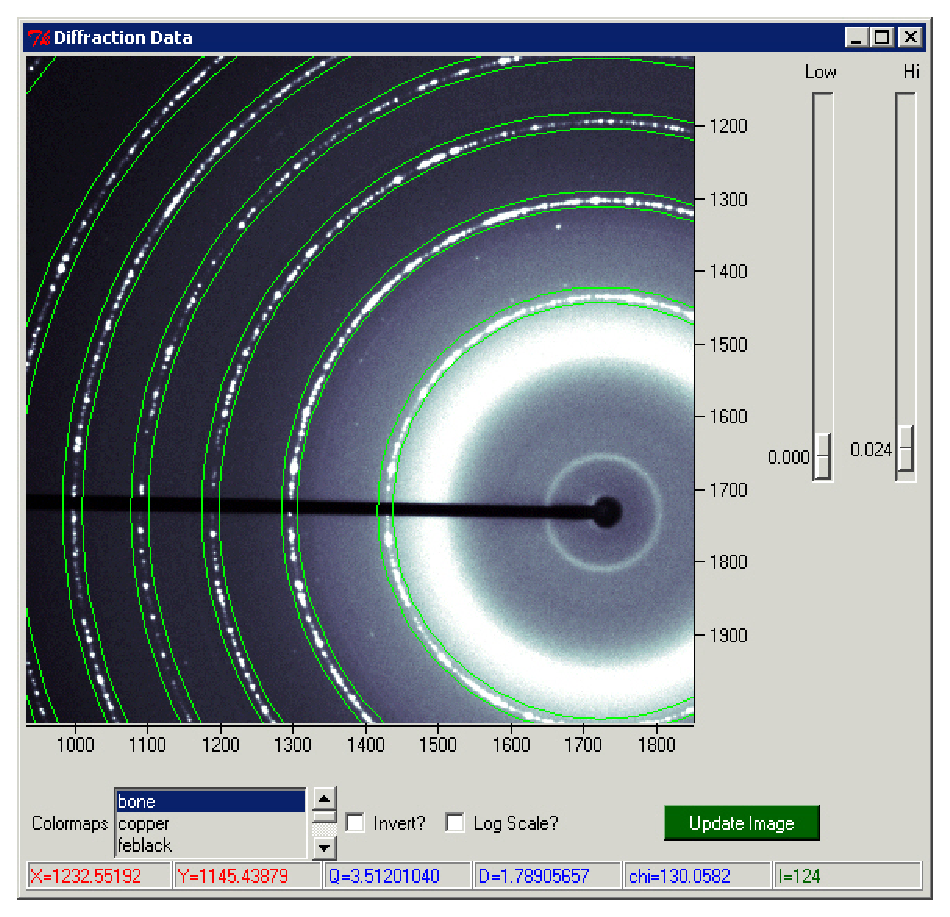
\includegraphics[scale=.75]{figures/constant_dq_lines_on_diffraction_image.eps}
    \caption{A division of a diffraction image into
    $Q$ ranges where each diffraction peak falls 
    uniquely inside one $Q$ range.}
    \label{divide_up_image}
\end{SCfigure}

\begin{SCfigure}[1][htbp]
\centering
% Generated with LaTeXDraw 1.9.5
% Sat Apr 26 21:57:04 EDT 2008
% \usepackage[usenames,dvipsnames]{pstricks}
% \usepackage{epsfig}
% \usepackage{pst-grad} % For gradients
% \usepackage{pst-plot} % For axes
\scalebox{1} % Change this value to rescale the drawing.
{
\begin{pspicture}(0,-4.41)(10.381406,4.41)
\pscircle[linewidth=0.04,dimen=outer](4.56,0.23){1.3}
\pscircle[linewidth=0.04,dimen=outer](4.451348,0.027117867){3.830909}
\psline[linewidth=0.04cm,arrowsize=0.1529cm 2.0,arrowlength=1.4,arrowinset=0.2]{->}(4.66,0.31)(8.76,2.91)
\usefont{T1}{ptm}{m}{n}
\rput(8.728282,3.72){\psframebox*[framesep=0, boxsep=false,fillcolor=white] {Constant $\chi$ Slice}}
\rput{-10.244087}(0.04480584,0.8143853){\pscircle[linewidth=0.04,linestyle=dashed,dash=0.17638889cm 0.10583334cm,dimen=outer](4.5651674,0.15725891){1.72815}}
\pscircle[linewidth=0.04,linestyle=dashed,dash=0.17638889cm 0.10583334cm,dimen=outer](4.56,0.21){0.8}
\pscircle[linewidth=0.04,linestyle=dashed,dash=0.17638889cm 0.10583334cm,dimen=outer](4.543829,0.0809504){3.2429092}
\pscircle[linewidth=0.04,linestyle=dashed,dash=0.17638889cm 0.10583334cm,dimen=outer](4.41,0.0){4.41}
\usefont{T1}{ptm}{m}{n}
\rput(8.951406,2.12){\psframebox*[framesep=0, boxsep=false,fillcolor=white] {$Q_2+\Delta Q_2$}}
\usefont{T1}{ptm}{m}{n}
\rput(7.911406,1.84){\psframebox*[framesep=0, boxsep=false,fillcolor=white] {$Q_2$}}
\usefont{T1}{ptm}{m}{n}
\rput(7.811406,1.52){\psframebox*[framesep=0, boxsep=false,fillcolor=white] {$Q_2-\Delta Q_2$}}
\usefont{T1}{ptm}{m}{n}
\rput(6.891406,0.84){\psframebox*[framesep=0, boxsep=false,fillcolor=white] {$Q_1+\Delta Q_1$}}
\usefont{T1}{ptm}{m}{n}
\rput(5.8714066,0.48){\psframebox*[framesep=0, boxsep=false,fillcolor=white] {$Q_1$}}
\usefont{T1}{ptm}{m}{n}
\rput(6.011406,0.04){\psframebox*[framesep=0, boxsep=false,fillcolor=white] {$Q_1-\Delta Q_1$}}
\psbezier[linewidth=0.04](6.8,1.67)(7.22,2.05)(6.9,2.53)(7.2,2.71)(7.5,2.89)(8.04,2.37)(8.32,2.63)
\psbezier[linewidth=0.04](4.94,0.49)(5.258421,0.81393445)(5.02,1.15)(5.2842107,1.2965574)(5.548421,1.4431148)(5.88,1.05)(6.1,1.23)
\end{pspicture} 
}


\caption{Here is a diagram of the peak finding algorithm. 
The solid circular black lines represent diffraction
peaks on the image. The dotted lines represent the
$Q$ ranges used to find the peaks. The diffraction
peaks are entirely within the ranges. Finally, the radial
line represents the program picking a particular $\chi$
value and looking for peaks inside of the $Q$ ranges.
Finally, the Gaussian peaks represent the program fitting
a gausian to the intensity profile inside of each of the
ranges.}
\label{fitting}
\end{SCfigure}

Our algorithm first requires\index{Peak Finding}
finding $(x,y)$ coordinates 
of many diffraction peaks. To do so, the algorithm will 
pick some $\chi$ value and then 
spread radially out from the center of the diffraction
image in this $\chi$ direction.\footnote{Remember
that the center is specified by the initial calibration 
values}. Between the given $Q$ range (for each of the $Q$ 
ranges), the program stores an array of all the data point 
on the line. It then fits a Gaussian to the data and the
$(x,y)$ coordinate of the center of this Gaussian $(x,y)$ 
is taken to be the peak. A diagram showing this algorithm
is shown in figure~\ref{fitting}. This method is
then done for many different evenly spaced $\chi$ values
and the particular value can be selected by the user
for increased accuracy.

The only really tricky part about this step is that
there is not always a consistent diffraction ring 
around the image and therefore some of these fits 
should not find peaks. Whenever this occurs, the program
just ignores the current fit and moves to the next. 
But figuring out when some particular peak is bad
is not particularly obvious. The method that this
program uses is to ensure each peak passes a few
tests. The first test is that the fit peak was
too close to the edge of the image. So any peak where
the Gaussian fit's center plus or minus twice the fit's
standard deviation gets outside of the $Q$ range is
considered too close to the edge of the image.
The next test that is done is to calculate is the
standard deviation of the data outside of the peak is
significant when compared to the height of the peak
fit. To do this, the code calculates the standard 
deviation of all the pixels that are farther then twice
the peak's fit standard deviation away from the
center of the peak. If the height of the peak
divided by this calculated background standard deviation
is smaller then some particular value, the peak is
considered bad. This value is called by the program
\gui{Stddev} and can be specified by the user from user.
\index{Stddev}
Presumably, the higher that \gui{Stddev} is, the
more picky the program is about what a good peak looks
like. This isn't the most robust method for finding peaks,
but it seems to work pretty well and it should be easy 
in principle to add new tests to the algorithm.

After compiling a list of diffraction peaks in the image,
the program can then define a residual function which
we can minimize to find the best fit calibration values.
To do so, we can convert the $(x,y)$ coordinate
of each of the peaks into a 
$(Q_{\text{peak}},\chi_{\text{peak}})$ pair. 
For each of these $(x,y)$ coordinates, we also
know what the input $Q$ list says the experimental $Q$ 
value for this peak should be (which we will call 
$Q_{\text{exp}}$). We can therefore define
the residual function as
\begin{equation}\label{residual}
    \text{Residual}(x_c,y_c,d,\lambda,\alpha,\beta,R) =  
        \sum_{\text{$x,y$ pairs}}
        (Q_{\text{peak}} - Q_{\text{exp}})^2
\end{equation}
The functional dependence comes from
calculating $Q_{\text{peak}}$ from a known
$(x,y)$ coordinate. We see that the smaller the 
Residual is, the closer we have come to finding 
the real calibration values which characterized
the diffraction experiment. If we had perfect
calibration parameters, the residual should be
equal to zero. But it is well defined for any
calibration parameters. So we can take this 
function of 7 variables and minimize it. 
The value of this function at its minimized 
is the best guess calibration values.
There are plenty of computer algorithm that
can minimize arbitrary multi-variable functions.
The one that this code uses is called the 
Levenberg-Marquardt\index{Least Squares Minimization}
nonlinear least squares algorithm
and the particular implementation that is used
to to perform the calibration is Manolis Lourakis's
levmar library\cite{lourakis04LM}. Ideally, 
once the minimization is done, a good guess at the
calibration values is found.

\section{Calibrating With the Program}

Diffraction image calibration is done with the
calibration tab of the program. This tab is shown 
in figure \ref{calibration_tab} on tab
\pageref{calibration_tab}.

As described above, to calibrate an image
you must have already loaded into the program
a diffraction data file, a $Q$ data 
file for the particular sample that was
taken, and an initial guess at the calibration 
data.

Once you have done these three things, you can
simply push the \gui{Do Fit} button to
calibrate the diffraction data. The program will
then perform the calibration algorithm as described
in section~\ref{cal_algorithm}. Once the program
finds a best guess for the new calibration
values, it will put those values into the inputs. 

While fitting the program will print to the
console some useful things. Most interesting,
the program will calculate the residual function
divided by the number of \ref{residual} and display
print the value to the terminal before and after
the calibration is done\footnote{Actually, the program
calculates the residual function divided by the number
of peaks. So it really displays the residual per peak, 
which is a more useful quantity because it would not
change if more peaks were used in the fit}
The output will look like
\begin{lstlisting}[caption={Displaying the Residual}]
 - Before fitting, the calculated residual is 5.336138e-04
 - Doing the fitting
 - After fitting, the calculated residual is 6.532131e-06
\end{lstlisting}
The program will then display the reason why the fitting
algorithm decided to quit doing the fitting and decided
that it found its best guess. For example, the program
might print out
\begin{lstlisting}[caption={Reason For Quitting}]
 - Reason for quitting the fit: 2-stopped by small gradient J^T e
\end{lstlisting}
The different reasons are told to me by the levmar fitting algorithm.
I am taking them directly from the levmar website
\url{http://www.ics.forth.gr/~lourakis/levmar/}
That website says that the different reasons why the
fitting can stop are:
\begin{itemize}
    \item stopped by small gradient J\verb!^!T e
    \item stopped by small Dp
    \item stopped by itmax
    \item start from current p with increased $\backslash$mu
    \item no further error reduction is possible. Restart with increased mu
    \item stopped by small $||$e$||$\_2\cite{lourakis04LM}
\end{itemize}
I think that the first reason to quit (stopped by smallw
gradient) means that the program found its way
to the bottom of the hill and is convinced that it did its best
job minimizing the function. I think that (stopped by itmax)
means that the program was forced to quit by a hard coded limit
to the number of loops through the fitting. So if you come across this
message, you should probably do the fit again with the current values.
I honestly don't know enough about the levmar fitting algorithm to
know what the other messages really mean. If you need to know, you 
should go into the fitting algorithm's documentation and see what you 
can find out.

The fitting algorithm also provides a covariance matrix that it finds
while fitting. I do now know how it calculates this matrix or what
it exactly what it means physically. Nevertheless, I print it out after the
fitting is done. 
\begin{lstlisting}[caption={Display of A Covariance Matrix},
    basicstyle=\ttfamily\footnotesize]
Covariance Matrix
[[  9.43e-04 -1.53e-04  5.36e-05  3.27e-03 -1.77e-03  3.64e-03  2.10e+00]
 [ -1.53e-04  1.17e-03 -1.40e-04 -8.58e-03  3.91e-05 -2.02e-04 -1.25e-01]
 [  5.36e-05 -1.40e-04  2.07e-04  1.38e-02 -1.45e-04  3.12e-04  1.78e-01]
 [  3.27e-03 -8.58e-03  1.38e-02  9.49e-01 -6.44e-03  1.40e-02  8.02e+00]
 [ -1.77e-03  3.91e-05 -1.45e-04 -6.44e-03  4.01e-01 -8.42e-01 -4.76e+02]
 [  3.64e-03 -2.02e-04  3.12e-04  1.40e-02 -8.42e-01  1.77e+00  9.99e+02]
 [  2.10e+00 -1.25e-01  1.78e-01  8.02e+00 -4.76e+02  9.99e+02  5.65e+05]]
\end{lstlisting}
The rows (from top to bottom) correspond to \gui{xc}, \gui{yc}, \gui{d}
\gui{E}, \gui{alpha}, \gui{beta}, and \gui{rotation}. The columns
(from left to right) also correspond to \gui{xc}, \gui{yc}, \gui{d}
\gui{E}, \gui{alpha}, \gui{beta}, and \gui{rotation}. I think that the
square root of the diagonal elements of the covariance matrix are supposed to 
correspond to uncertainties, but I do not know enough about the minimization
algorithm to be really comfortable saying that these are the true uncertainties in
the fit parameters. Your mileage my vary. Anyway, I print out the root of the 
diagonals. The printout by the program  
\begin{lstlisting}[caption={Display of the root of the diagonals}]
Root of the diagonal of the covariance matrix ... 
xc:  0.0307145820046
yc:  0.0341970790239
d:  0.0143735880013
E:  0.97393322373
alpha:  0.633295666676
beta:  1.32940880588
rotation:  751.595873785
\end{lstlisting}
    
If you do not like the guess for the calibration 
parameters, you can always unto to the previous
calibration values before the fit using the
\gui{Previous Values} input.

\section{\texorpdfstring{The \gui{Number of Chi?} 
        and \gui{Stddev?} Input}{The Number of 
        Chi and Stddev Inputs}}

The calibration algorithm requires starting
at the center and moving across the image in constant
$\chi$ slices (see section~\ref{cal_algorithm} or 
figure~\ref{fitting} for a graphical representation).
The number of these slices around the image that
should be done is user selectable using the 
\gui{Number Of Chi?} input. The default value is 360.
The more $\chi$ slices that are used, the slower
the fit will be.

Section \ref{fitting_sec} describes how the program
uses a parameter to determine how picky it should
be in allowing peaks that it finds. Roughly, this
parameter corresponds to how many times larger
the peak has to be then the background noise outside
of the peak. This parameter can be set using the 
\gui{Stddev?} input. The default value is 5. The higher 
the value, the less likely the program will be to find
and use bad peaks but the more likely it will be to
ignore valid good peaks.

\section{\texorpdfstring{Work in 
    $\lambda$}{Work in Lambda}}
    \label{workWavelength}

Often times, one wishes to deal with the wavelength 
of the incoming beam of light instead of the energy
of the beam. Of course, the energy and wavelength
are intemately related by the formula
\begin{equation}
    E=hc/\lambda
\end{equation}
If you wish to work with wavelength in units of
nanometers instead of energy in units of electron 
volts, you can change the state of the program so 
that the program works with wavelength instead
of energy. To do so, you have to go into the menu bar
and change the radio select from \gui{Work in eV}
to \gui{Work in Lambda}. Once you do that, the 
calibration parameter input will be labeled
$\lambda$. Any number in that input will then be converted.
After the parameter is modified during a fit,
the program will put the wavelength value into
the input. Finally, when the calibration
parameters are saved to a file, the wavelength will
saved to the file instead of the energy.


\section{Fixing Calibration Parameters}
\label{fix_parameters}

When fitting calibration parameters, it is not
always desirable to allow the program to vary
all of the calibration parameters. For example,
the energy of the beam used during the diffraction
experiment might be already very well known already
so there would be no reason to calibrate the energy.
If you wish to fix any of the calibration parameters
values so that it does not vary during a calibration
fit, you can use the check boxes under the \gui{Fixed?}
label to fix the parameter. When the corresponding
check box is checked, the parameter will not vary
during the fit. When it is not checked, the
parameter will vary during the fit. You
can not fix the pixel length and 
pixel height because they are always held fixed. This is 
because these are never
the short of thing that one would want to vary.
They are some property of the detector that is known in
advance.

\section{\texorpdfstring{Displaying Constant $Q$ 
    Lines}{Displaying Constant Q Lines}}
    \label{displayconstQlines}

After the program has been given a diffraction file,
a list of the constant $Q$ lines, and some
calibration parameters, the program has a very
useful feature where it can display on top of
the image the diffraction pattern that should
show up for the particular $Q$ lines and the
particular calibration parameters.

The \gui{Draw Q Lines?} button on the 
\gui{Calibration} tab enables this.
Figure~\ref{constant_q_lines_on_diffraction_image}
shows what the diffraction image looks like with
the $Q$ lines drawn on it.

\begin{SCfigure}[1][htbp]
    \centering
    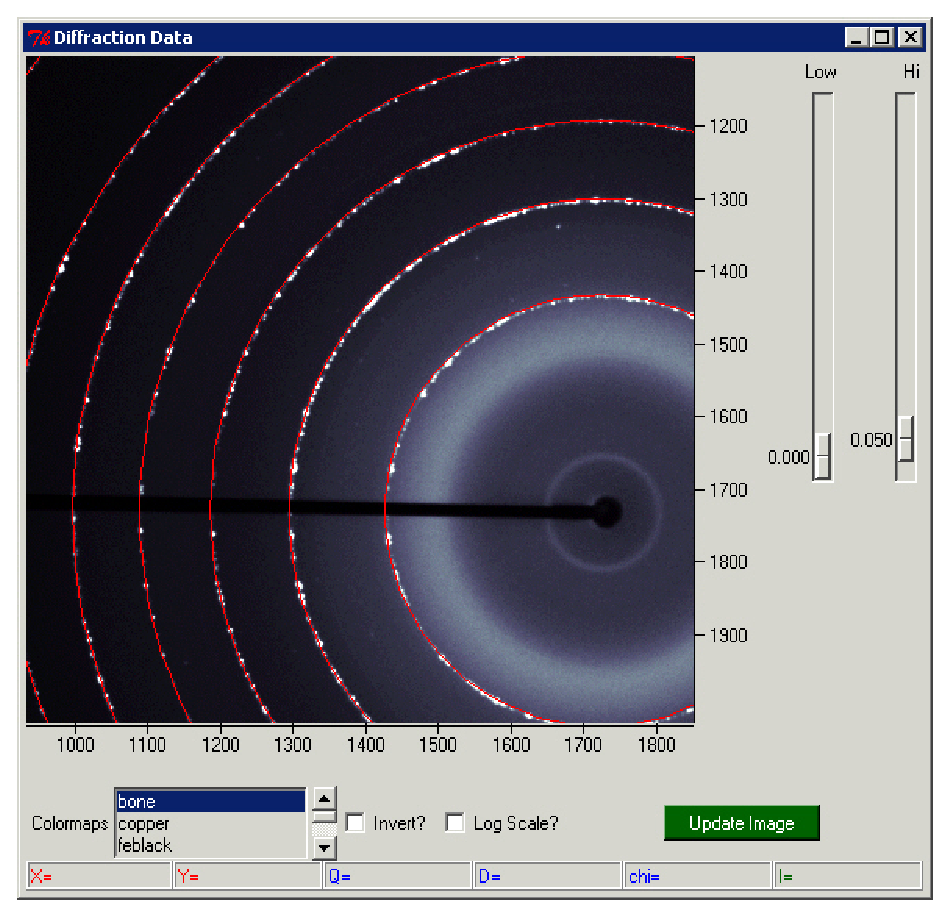
\includegraphics[scale=.75]{figures/constant_q_lines_on_diffraction_image.eps}
    \caption{A diffraction image with constant the 
    $Q$ lines displayed on it.}
    \label{constant_q_lines_on_diffraction_image}
\end{SCfigure}

Drawing these lines is actually very easy. For
each $Q$ value, the program picks a lot of
$\chi$ values. We know that each of the $Q$, $\chi$
values is in the constant $Q$ line so we can use
the calibration parameters to convert them to $x$, $y$
values and connect all the pixel coordinates to 
make the line.

Constant $Q$ lines can also be drawn on top of the
caked data. This is described in 
section~\ref{cakeQlinesandpeaks}.  
The color of the $Q$ lines can be changed using the
\gui{Color} button next to the \gui{Draw Q Lines?} 
button.

\section{\texorpdfstring{Displaying Constant $\Delta Q$ 
        Lines}{Displaying Constant delta Q Lines}}
        \label{displayconstdQlines}
        

The program needs in addition to the $Q$ values
a range in $Q$ to find the peaks. See 
section~\ref{fitting_sec} for more details. Because
the program has this range, it can also display the
$\Delta Q$ range on top of the image.
This can be done with the \gui{Draw dQ Lines?} button
and the color of these lines can be changed with the
corresponding \gui{Color} button. 
Figure~\ref{constant_dq_lines_on_diffraction_image}
shows what the diffraction image looks like with
the $\Delta Q$ lines drawn on it.

\begin{SCfigure}[1][htbp]
    \centering
    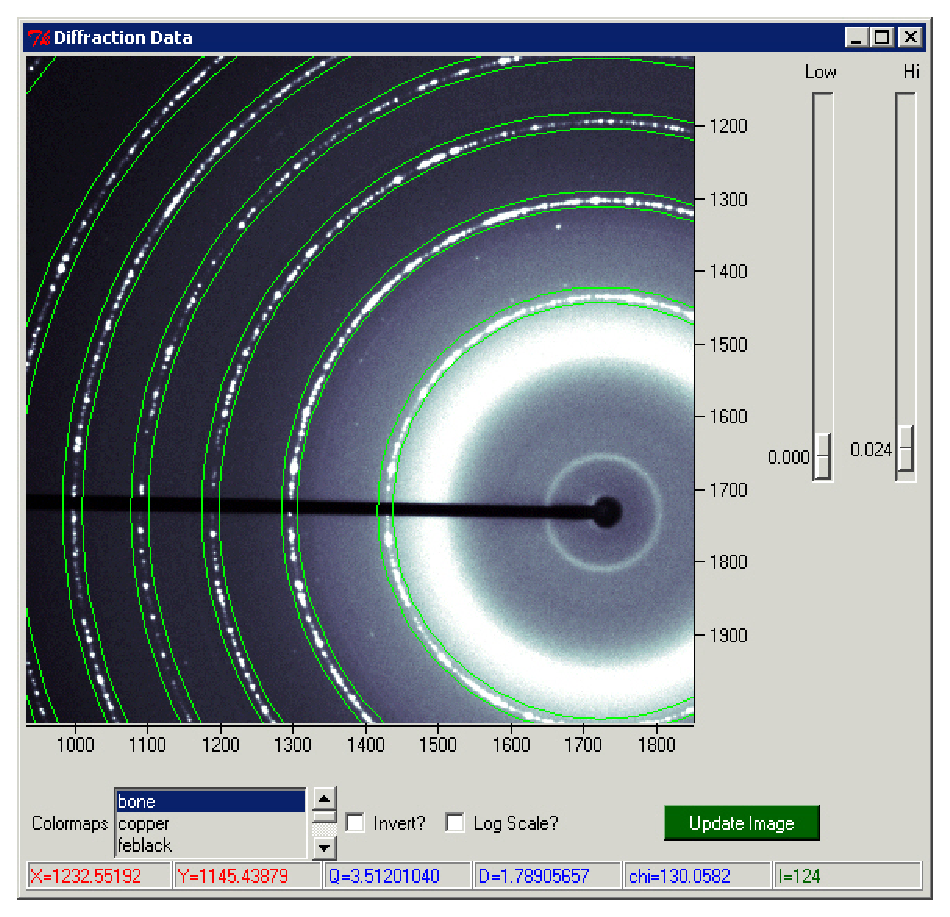
\includegraphics[scale=.75]{figures/constant_dq_lines_on_diffraction_image.eps}
    \caption{A diffraction image with the constant 
    $\Delta Q$ lines displayed upon it.}
    \label{constant_dq_lines_on_diffraction_image}
\end{SCfigure}


Constant $\Delta Q$ 
lines can also be drawn on top of the caked data. This 
is described in section~\ref{cakeQlinesandpeaks}.

\section{Displaying Peaks}\label{displaying_peaks_diffraction}

Section~\ref{fitting_sec} describes how the program has to find a bunch
of peaks on the diffraction image in order to perform the calibration.
After the program has found all the peaks, it can conveniently display
them on top of the diffraction image. This can be done with the
\gui{Draw Peaks?}. The peaks will be displayed as crosses and the color
of the peaks can be changed with the corresponding \gui{Color} button.
Figure~\ref{peaks_on_diffraction_image} shows what the diffraction image
looks like with the peaks drawn on it. This feature is useful because 
you can use it to see if the program is actually finding real peaks
corresponding to diffraction maxima. If many of the peaks that the program 
finds do not correspond to diffraction maxima, it is less likely that 
the program would do a good job calibrating the diffraction image.

\begin{SCfigure}[1][htbp]
    \centering
    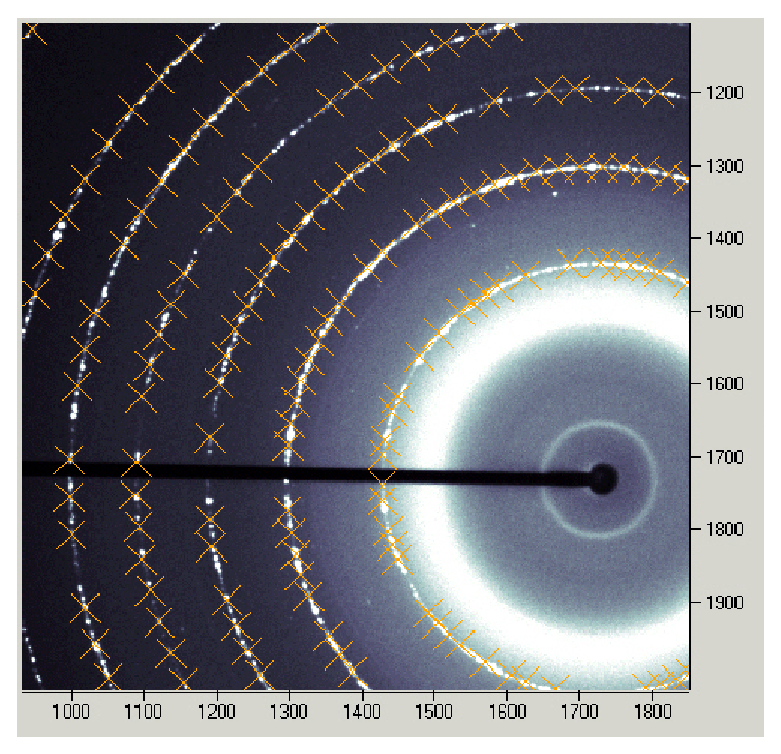
\includegraphics[scale=.75]{figures/peaks_on_diffraction_image.eps}
    \caption{A diffraction image with the peaks displayed upon it.}
    \label{peaks_on_diffraction_image}
\end{SCfigure}

Peaks can also be drawn on top of the caked data. This 
is described in section~\ref{cakeQlinesandpeaks}.

\section{Masking Peaks}

\begin{figure}[htb]
    \centering
    \subfloat[A diffraction image with diffraction peaks
    and two polygon masks displayed on top of it.]{
    \label{mask_peaks_diffraction}
    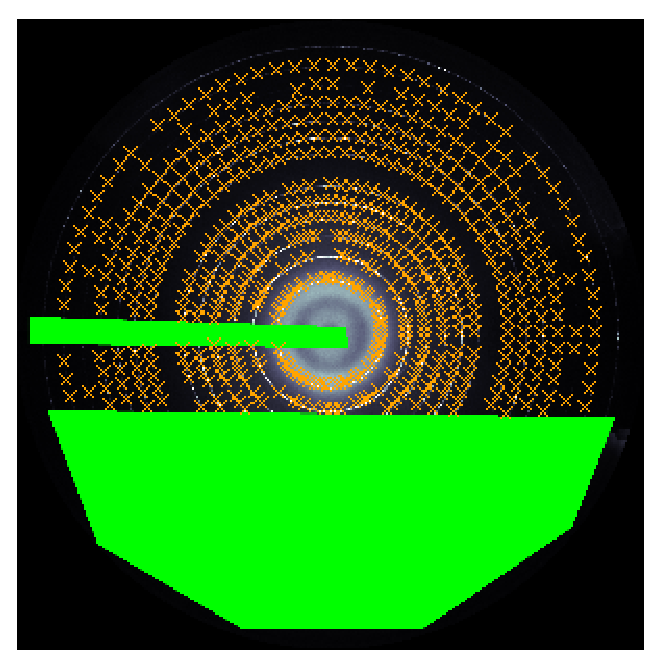
\includegraphics[scale=.75]{figures/mask_peaks_diffraction.eps}}\;\;
    \subfloat[A caked plot with diffraciton peaks and
    two polygon masks displayed on top of it.]{
    \label{mask_peaks_cake}
    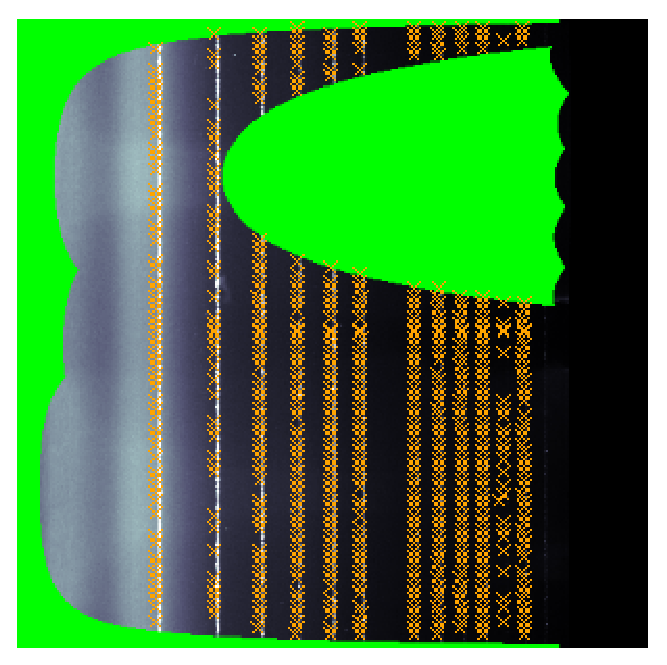
\includegraphics[scale=.75]{figures/mask_peaks_cake.eps}}
    \caption{Polygon masks can be used to block
    out certain regions of the image. Whenever
    a polygon mask is loaded into an image, none
    of the peaks found in the mask's region will be
    used while calibrating the image. Furthermore,
    none of the peaks within the masks will be 
    displayed on the diffraction image or caked plot.}
    \label{mask_peaks}
\end{figure}

The general idea behind masking peaks is allow polygon 
masks (see chapter~\ref{pixel_masking}) to be used as 
a way to forbit the program from using any peaks found
within a certain region. So if a polygon mask covers a 
certain area of the image, none of the peaks found within that
area will be used while calibrating. Also, none of 
the peaks will be displayed on top of the diffraction 
image or cake image. An example of this is shown in
figure~\ref{mask_peaks_diffraction}. 
See section~\ref{displaying_peaks_diffraction}
for a discussion of displaying peaks on a diffraction
image.  Figure~\ref{mask_peaks_cake} shows the same effect 
on top of the corresponding caked plot. See 
chapter~\ref{Caking} for a discussion of caking.
In particular, see section~\ref{displaying_peaks_cake} 
for more information on displaying peaks on a caked
image. This feature was added in version 2.0.0.

\section{Saving the Peak List}

The program has a feature where it can generate
a list of diffraction peaks that it finds the 
diffraction image (just like when it is calibrating)
but then instead of calibrating the image, the program
saves out all of the peaks to a data file. This can
be useful, for example, if you need a list of pixel 
coordiantes where diffraction peaks are for some further
data analysis. The \gui{Make/Save Peak List} button can
be used to save out the peak list. Just as in calibrating,
the program requires in advance for a diffraction file to
be loaded, for a standard $Q$ file to be loaded, and for
a guess at the calibration parameters to be in the inputs.

A typical peak list file looks like\footnote{I have modified
what a real file looks like a bit. The numbers are really tab 
separated but I show them space separated for brevity.}
\begin{lstlisting}[caption={A Peak List File,basicstyle=\ttfamily\tiny}]
# A list of peaks found in the diffraction image.
# Calculated on Sun Apr  6 18:06:56 2008
# Calibration data used to find peaks:
#   x center:    1725.0000000 pixels
#   y center:    1725.0000000 pixels
#   distance:     122.5040000 mm
#   energy:     12714.2388941 eV
#   alpha:          0.0000000 degrees
#   beta:           0.0000000 degrees
#   rotation:       0.0000000 degrees
#   pixel length:     100.0000000 microns
#   pixel height:     100.0000000 microns
#   x  y  RealQ  FitQ  chi  width  intensity  2theta
2016.15  1724.44  1.511  1.50  0.11  0.0075 5564.32  13.36
2016.68  1719.33  1.51  1.50  1.11  0.0093 1662.72  13.39
\end{lstlisting}
First, the file contains the calibration parameters
used to generate the peaks. Then it has a comment string
describing each of the numbers in each of the rows
that follow. Each row corresponds to a unique peak.
The first two numbers $x$ and $y$ are
the $x$ and $y$ pixel coordinate corresponding to
a location in the diffraction image of the peak. RealQ 
is the $Q$ value found in the $Q$ list that is already 
known. FitQ is the $Q$ value calculated 
from the $(x,y)$ coordinate using the calibration
parameters. $\chi$ is also calculated from the pixel
coordinate using the calibration parameters. 
Intensity is intensity value found in the data at
this peak. $2\theta$ is calculated at the $(x,y)$ 
coordinate using the calibration parameters.

\section{Handling Calibration Data}

There are inputs in the calibration tab of the
program for input of the calibration parameters.
\gui{xc} is for the $x$ center, \gui{yc} is
for the y center, \gui{d} is for the distance,
\gui{E} (or \gui{$\lambda$:}) is for the energy
or wavelength. The $\alpha$, $\beta$, and
$R$ inputs are for the three angles. 
\gui{pl} stands for the pixel length
and \gui{ph} stands for the pixel height.

You can directly input calibration data using 
the inputs and once the data is in the inputs
it can be used by the program to do the calibration
(or the caking or anything else).

But there are a couple of other ways to deal
with calibration data.
You can load and save calibration program
from the program using the \gui{Load From File}
and \gui{Save To File} buttons. This is nice
because it can be used, for example, to save 
the data that was found by calibration data
for future reference. As you will see, the 
calibration data files can handle information
about whether the parameters should be fixed
(see section \ref{fix_parameters}).

The format for a calibration data file is 
pretty simple. Below is  an example
\begin{lstlisting}[caption={Calibration Parameters}]
# Calibration File
xc	1725.000000	0
yc	1725.000000	0
D	125.296000	0
E	12735.395772	0
alpha	0.000000	0
beta	0.000000	0
rotation	0.000000	0
pixelLength	100.000000
pixelHeight	100.000000
\end{lstlisting}
Comment lines beginning with
a \# and are ignored. Each of the parameters
gets its own line. Each parameter name is 
followed by some spaces or tabs and then the
value. The value can be followed by an optional
second number which is either zero or one.
The second number corresponds to whether or
not the parameter should be fixed while
fitting. One means fix the parameter. Zero means
let it very. If no number is given, the default
is to not fix the parameter.

Instead of energy, the wavelength of the incoming
beam of light can be stored in a calibration file.
The wavelength line would look like 
\macroline{wavelength	0.973540}.
When the program is in wavelength mode, the program
will save out calibration parameters with this line
instead of the one above. The program will load in a 
file containing either no matter what mode the program 
is in. It will do the conversion if it has to do put 
the right value into the input. See 
section~\ref{workWavelength}.


\section{\texorpdfstring{Handling $Q$ Data}{Handling Q Data}}
\label{TheQValues}\index{Q Data}

$Q$ data is always loaded into the program from files. 
$Q$ data can be loaded into the program with the \gui{Q Data:}
input on the calibration tab. 
You can either type in the filename of the $Q$ file by hand 
and push the load button or click on the folder icon to the 
side and use the file selector to pick the file that you want.

The $Q$ data file format is pretty simple. Below is an example 
\begin{lstlisting}[caption={Lanthanum Hexaboride.dat},label=LaB6]
# This is Q Data for Lanthanum Hexaboride
Q   dQ
1.511543809 .05
2.137646823 .05
2.618102966 .05
3.023087619 .05
3.379873753 .05
3.702525225 .05
...
\end{lstlisting}
Comment lines beginning with a \# and are always ignored. The
first line in the file should be of the form "Q  dQ" or "Q  delta Q" 
to specify that this is a list of $Q$ values. The rest of the
file should have $Q$ values followed a $\Delta Q$ range.
All $Q$ values must be larger than 0. None of the $Q$ ranges can 
overlap. Instead of inputting $Q$ values, the program can input
$D$ values if the first line is instead "D dD" or "D delta D"
The values should be given instead in $D$ space and the values
will be converted using~\ref{DtermsQ}.

\section{\texorpdfstring{The \gui{Get From Header?} Input}
    {The ''Get From Header Input''}}

Often times guesses at the experimental parameters are 
stored in the header data inside of the diffraction image. 
The program can try to find these header calibration parameters
and put them into the calibration parameters inputs in the 
program. This can be done with the \gui{Get From Header} 
button.





When analyzing diffraction dat, not all of the pixels in 
an image should be used in the analysis. In order to make 
the program
ignore certain pixels when doing the analysis, this
program allows for two types of pixel masking:
threshold masking and polygon masking. You can 
apply either of these from the 
\gui{Masking} tab. figure~\ref{masking_tab}
shows this tab. 

\section{Threshold Masking}

\begin{SCfigure}[1][htbp]
    \centering
    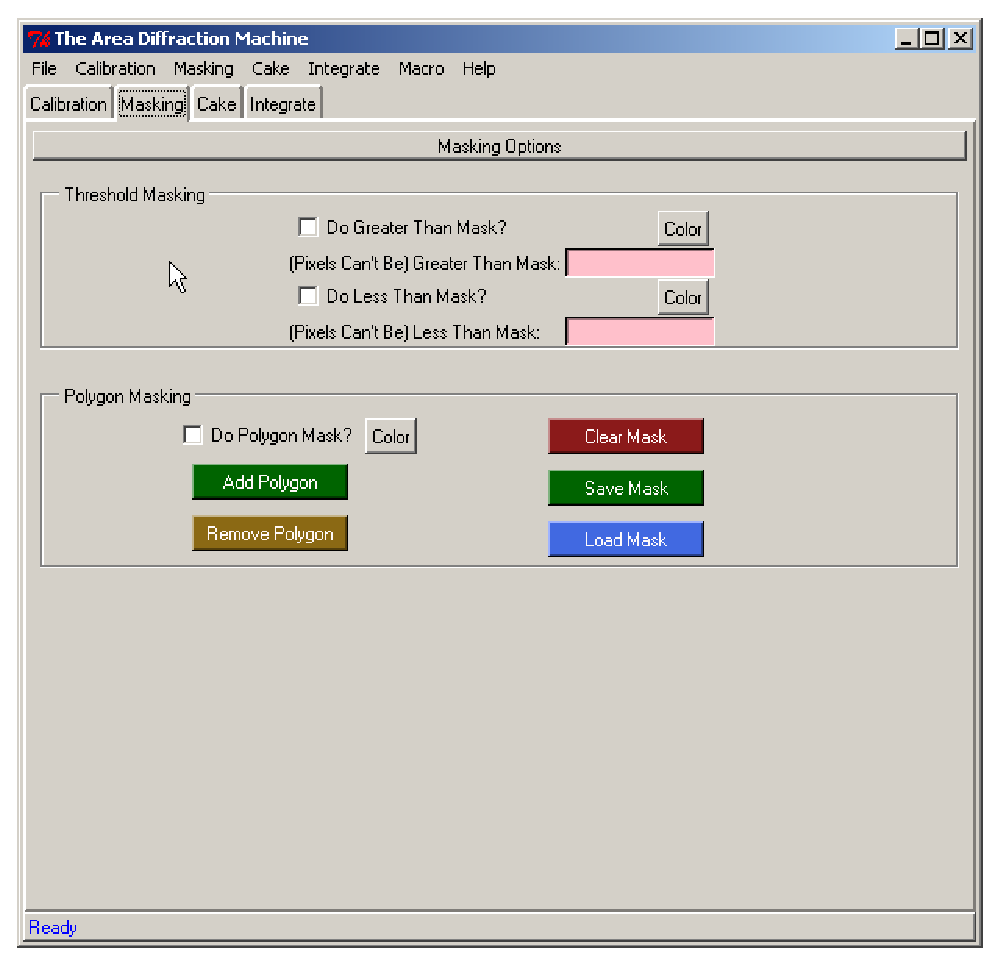
\includegraphics[scale=.75]{figures/masking_tab.eps}
    \caption{The pixel masking tab. It allows for threshold 
    masking and polygon masking.} 
    \label{masking_tab}
\end{SCfigure}

The top half of the \gui{Masking} tab is devoted to 
threshold masking. Threshold masking allows all pixels, 
either above a certain intensity or below a certain 
intensity, to be ignored when doing the diffraction 
analysis. The \gui{Do Greater Than Mask?} check box can 
be used to apply a mask that will cause all pixels 
greater than a certain value to be ignored.
The \gui{(Pixel's Can't Be) Greater Than Mask} input 
can be used to specify the maximum pixel value.
Correspondingly, the \gui{Do Less Than Mask} check box
can be used to make the program ignores all
pixels below a certain value. The particular value can 
be specified with the \gui{Less Than Mask} input. 

\begin{SCfigure}[1][htbp]
    \centering
    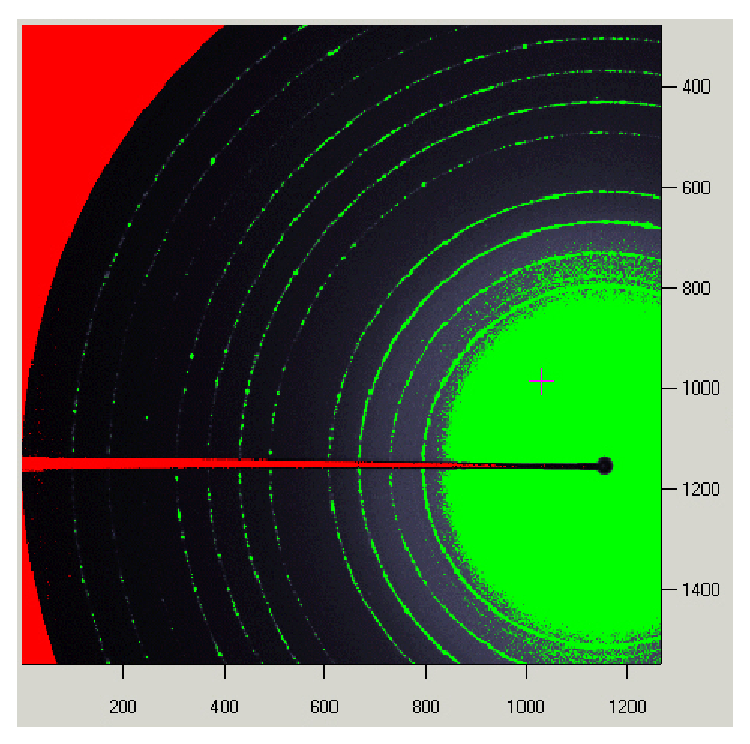
\includegraphics[scale=.75]{figures/Threshold_Masking.eps}
    \caption{A diffraction image with a
    greater than mask and less than mask.
    All pixels with intensity greater than 5000 
    have been colored green. All pixels with 
    intensity less than 30 have been colored red. Applying
    an intensity mask can be a useful way to see if a detector's
    pixels have been overloaded. They can also be a used to
    ensure that no overloaded pixels are used in subsequent
    data analysis.}
    \label{Threshold_Masking}
\end{SCfigure}

When you apply a threshold mask, the pixels over this threshold 
will all be colored differently on the diffraction and cake image. 
You can specify what you want these masked to be colored 
with the \gui{Color} button next to the greater 
than and less then masks. Figure~\ref{Threshold_Masking} shows 
what a diffraction image looks like when all pixels
with intensity above 5000 are colored green and all pixels 
below 30 are colored red.

When caked data is saved out to a file, any of the pixels 
that are larger than the greater than mask are saved 
as -2. Any of the pixels smaller than the less than mask
are saved as -3.  If you need to analyze caked data outside 
the program, this behaviour needs to be accounted for.

When an intensity integration is saved to a file, 
any of the too high or too low pixels are simply ignored when 
calculating average intensity. 

\section{Polygon Masking}

\begin{SCfigure}[1][htbp]
    \centering
    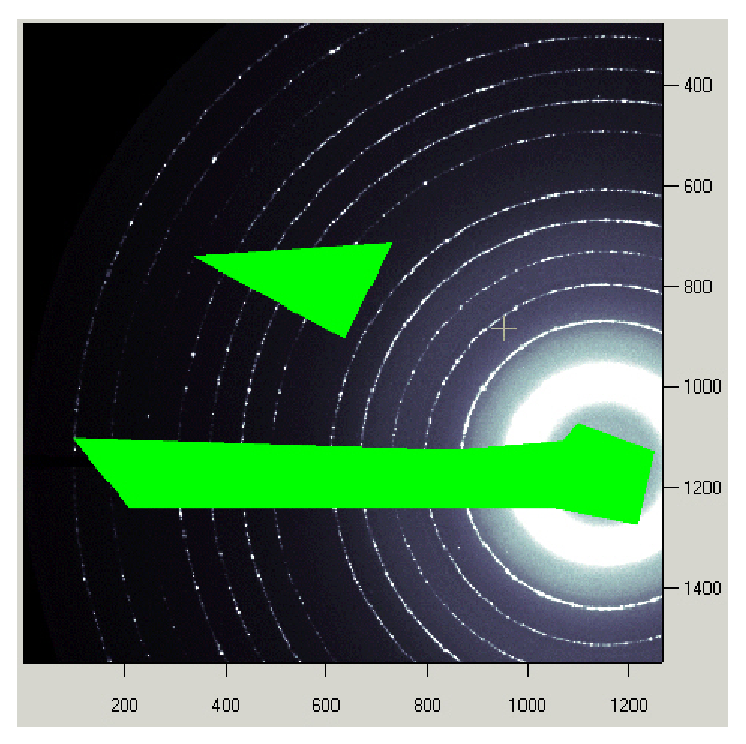
\includegraphics[scale=.75]{figures/Displayed_Polygon.eps}
    \caption{Here are two polygon masks that have been applied
    to a diffraction image. One of them blocks the beam stop.}
    \label{Displayed_Polygon}
\end{SCfigure}

Sometimes, large areas of a diffraction image should not
be included in any data analysis. For example, 
often a beam stop blocks part of the detector
and the pixels behind the beam stop should be ignored. 
To allow for this sort of masking, the program has a 
polygon masking feature. Polygons can be drawn around 
certain parts of the diffraction image and those parts 
of the image will not be used in any subsequent analysis. 
This program can handle multiple polygons at the same time.

So long as the \gui{Do Polygon Mask?} check box is
selected, the polygon masks will be used 
when performing subsequent analysis. 
The polygons will be displayed on the diffraction and cake image. 
Any pixel in the diffraction or cake image that is inside one of
the polygons will have a different color.
An example of polygons on a diffraction image are 
shown in figure~\ref{Displayed_Polygon}.
The color of the polygon masks can be changed using 
using the \gui{Color} button
next to the \gui{Do Polygon Mask?} check box.
When caked data is saved out, any pixels inside 
polygon masks will be given an intensity 
value of -4. During an intensity integration 
masked pixels will be ignored.

\begin{SCfigure}[1][htbp]
    \centering
    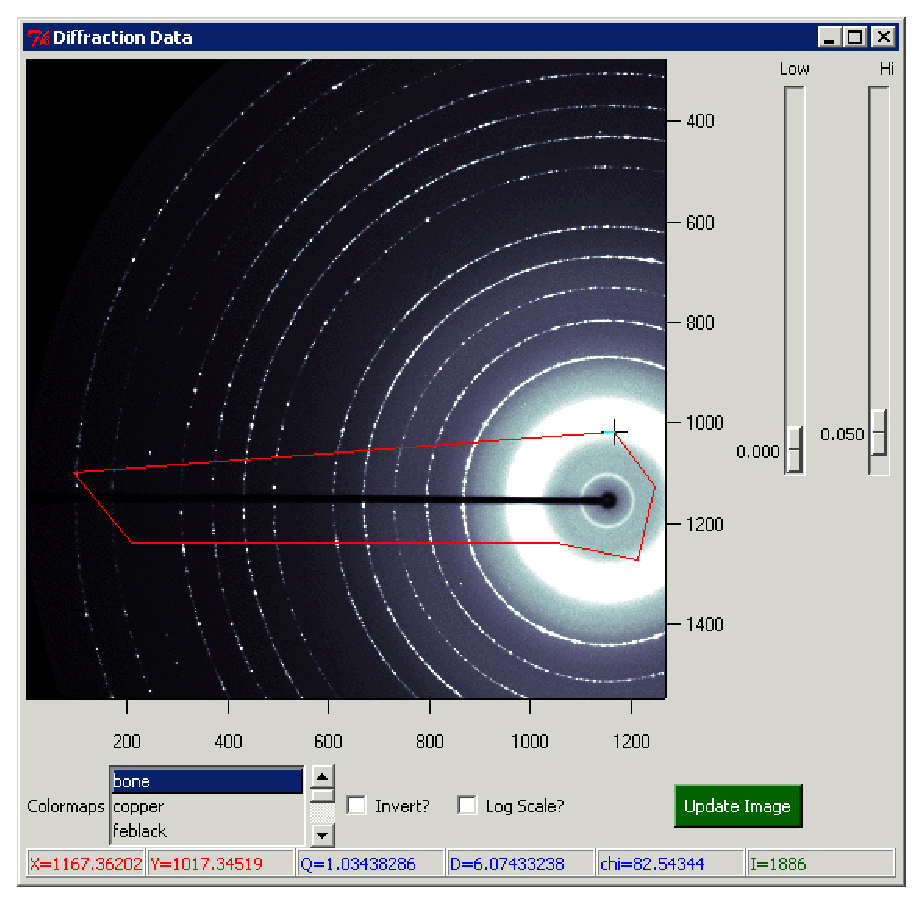
\includegraphics[scale=.75]{figures/Adding_Polygon.eps}
    \caption{Here is the interface for adding a new polygon 
    mask to the program. This particular mask will cover 
    the beam stop so that the beam stop does not affect
    the intensity integration.}
    \label{Adding_Polygon}
\end{SCfigure}

A polygon mask can be added to the image by pushing
the \gui{Add Polygon} button on the \gui{Masking} tab. 
This button will stay down when pushed.  Pushing it puts 
the program in polygon drawing mode.  In this mode, the 
diffraction image will behave differently. The diffraction
image can no longer be zoomed or panned.
Instead, left clicking on the diffraction image will make
the program draw the polygon.  The first left click adds the
first vertex. Each success left click add another vertex. 
The drawing can be finished by right clicking (this will
also create a final vertex). Right clicking will make
the program exit the drawing mode, return to its
original state, and add the polygon into the program. 
Multiple polygons can be added using the \gui{Add Polygon}
button. Figure~\ref{Adding_Polygon} shows 
the program when a polygon is
being drawn. Drawing a polygon can be aborted without
saving the mask by unpushing the \gui{Add Polygon} button.

\begin{SCfigure}[1][htbp]
    \centering
    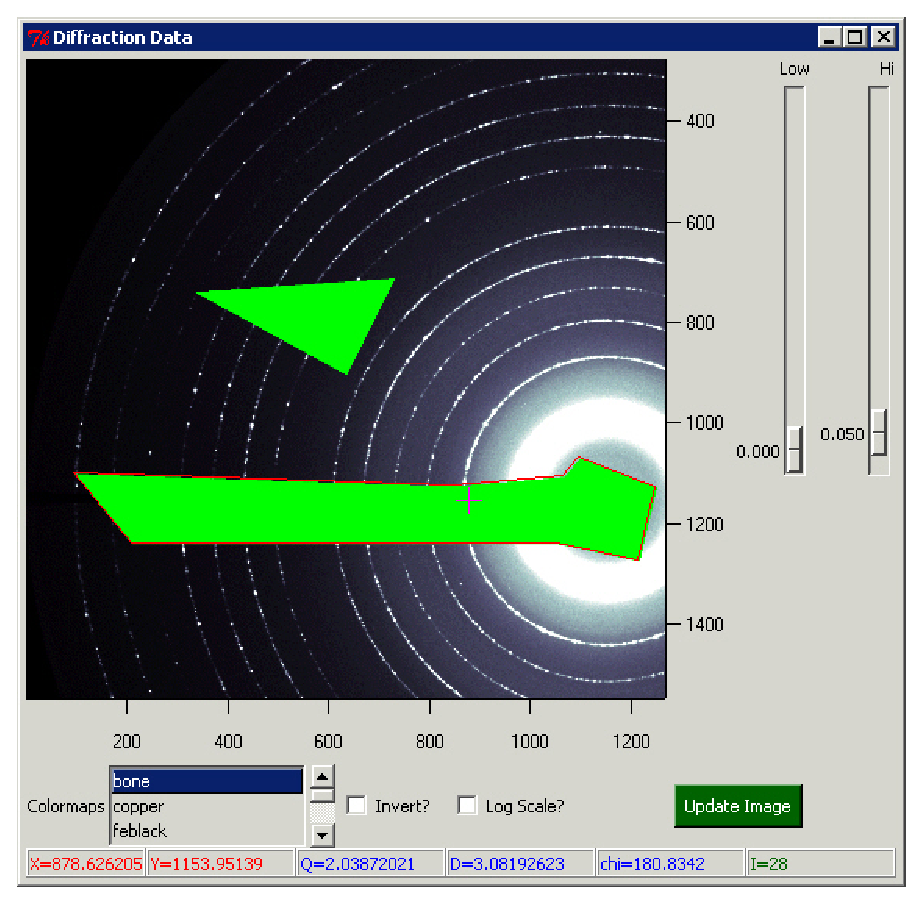
\includegraphics[scale=.75]{figures/Removing_Polygon.eps}
    \caption{Here is the diffraction
    image window as a polygon is about to be removed.
    When mousing over a polygon to remove it,
    the program will display a red border around it.}
    \label{Removing_Polygon}
\end{SCfigure}

The \gui{Remove Polygon} button can be used to remove
a polygon in the program. Like the \gui{Add Polygon} 
button, this button will stay pushed and change the
behavior of the diffraction image. After the 
\gui{Remove Polygon} button is pushed, clicking over
a particular polygon will remove it.
After the polygon is removed, the program will 
return to its normal state.
Figure~\ref{Removing_Polygon} shows what the diffraction
window looks like when a polygon is about to be removed.
The program can be returned to its normal state without
removing a polygon by unpushing the \gui{Remove Polgyon}
button.

The \gui{Clear Mask} button can be used to remove
all the polygons at once. The \gui{Save Mask} button
can be used to save all the polygons to a file.
A file of polygons can be added to the program 
using the 
\gui{Load Mask} button. The file for polygon
files is very simple. For the polygons in 
figure~\ref{Displayed_Polygon}, the following
file would be saved:
\begin{lstlisting}[caption={'polygons.dat'}]
# Polygon(s) drawn on Thu Feb 07 00:00:21 2008
93.140587183	1098.06704199
208.013978042	1237.77792276
1052.48863517	1237.77792276
1213.93231962	1271.92947139
1248.08386825	1126.00921814
1095.95424252	1067.02017959
1064.90738013	1104.27641447
847.579343365	1122.9045319

332.201427619	737.923438212
633.355992844	902.471808902
729.601266267	709.981262058
\end{lstlisting}
Each line is an ($x$,$y$) coordinate for one of 
the nodes of a polygon.  The coordinates are separated
by spaces. Each polygon is separated by a newline.  
Comment lines beginning with \# are 
ignored. 

\section{Masking Caked Plots}

\begin{figure}[htb]
    \centering
    \subfloat[A rectangular polygon mask in 
    the middle of a diffraction image]{
    \label{box_mask_diffraction}
    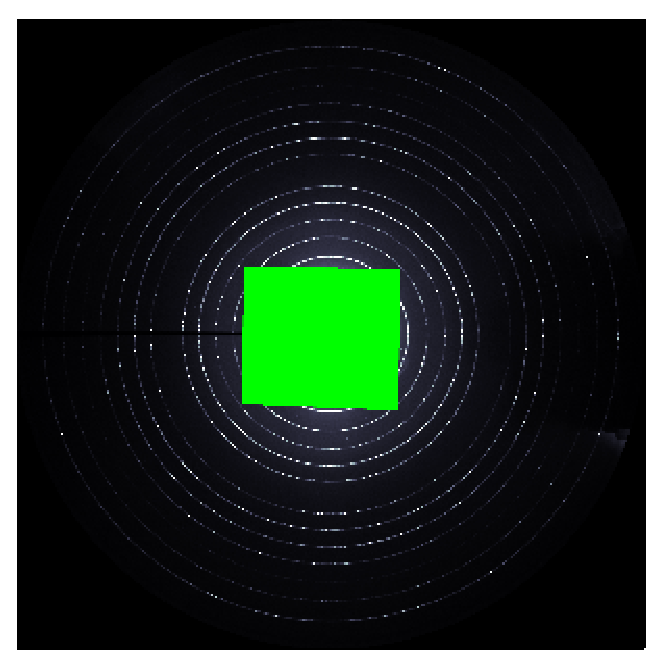
\includegraphics[scale=.75]{figures/box_mask_diffraction_image.eps}}\;\;
    \subfloat[The same rectangular mask on
    a caked plot]{
    \label{box_mask_cake}
    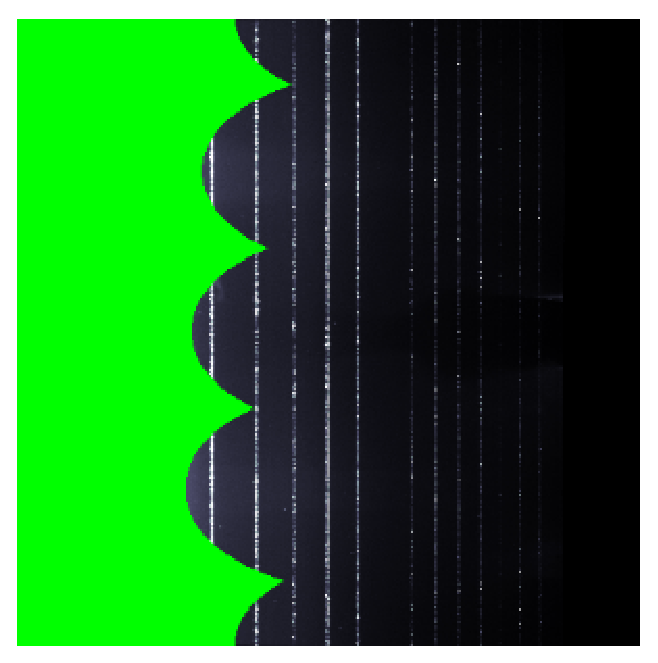
\includegraphics[scale=.75]{figures/box_mask_cake_image.eps}}
    \caption{An example of how a relatively simple
    shape on a diffraction image will can look very
    different on a caked plot.}
    \label{box_mask}
\end{figure}

Any polygon mask or threshold mask will also 
show up on the caked plot. Polygons on the 
diffraction image can look very distorted on 
caked plots. Figure~\ref{box_mask} shows an example.





\begin{center}
    {\em ``Let Them Eat Cake''} -- Maria Theresa of Spain 
\end{center}

\subsection{The Cakeing Algorithm}

The purpose of a caked plot is to make a radial 
($r$ vs $\theta$) plot of the data as it would have 
appeared on the imagined untiled detector shown in 
figure~\ref{PhysicalSetup}. By plotting $r$ vs $\theta$,
we will turn circle (of constant $r$ into straight lines 
and we will really distort straight lines.
To create this plot, we will work with the 
convenient quantities $Q$ and $\chi$. Remember that
from equation \ref{qterms2theta} that $Q$ is
related by the sin function to $2\theta$ and that
from equation \ref{2thetatermsr} that $2\theta$
is related to the distance $r$ on the untilted 
detector by the tangent function. 
Consequently, although the relationship is not 
strictly linear, $Q$ will increase as $r$ increases
and therefore $Q$ is an analogous quantity to $r$.
Also, $\chi$ directly meausres teh angle radially
around the center of the image. So a cake is really
defined as an intensity plot of the diffraction 
image where the two axis are $Q$ and $\chi$.

To calculate a cake plot, the program implements
the following algorithm. The program has to somehow bin $Q$ and 
$\chi$ space. The code itself can try to pick
a range large enough to encompase all of the 
pixels inside of the diffraction image. Alternately,
the user can specify by hand the exact range that
they want to have caked. But once the bins are
specified, the program has to fill each bin with
intensity values. Since each bin has some 
particular $Q$ and $\chi$ value\footnote{Technically,
each bin has a $Q$ and $\chi$ range, but we will
take the middle of each of these ranges to be the
particular $Q$ and $\chi$ value corresponding to the
bin.} we can calculate the corresponding $(x''',y''')$
pixel coordinate for this bin using 
(USE EQUATION FOR INVERTED EQUATION). We can then
look inside the loaded diffraction data for
this particular intensity value corresponding
to the $(x''',y''')$ value. This intensity then
gets placed inside the bin. $(x''',y''')$
is generally a floating point number so we should
do a bilinear interpolation of the intensity values
to get a best guess.

In principle, the caking algorithm could be implemented
differently. The way it is coded up is to loop over
all the bins. But one could equally well have looped over
all the pixels of diffraction data. Each pixel has a
particular $(x''',y''')$ coordiante. We could use
equations~\ref{ytermsydoubleprime} and
equation~\ref{xtermsxdoubleprime} to calculate the $Q$
and $\chi$ value corresponding to this coordiante. We
could then add the intensity value corresponding to the
$(x''',y''')$ value into the bin which contains the
$Q$ and $\chi$ value. After doing this for all the pixels
in the image, we could then average all the cake bins.
This method would be more accurate because each of the 
pixels in the diffraction image would be used in the analyis
where as they are not necessarily all used above. The major
downside to this implementation is that it does not 
necessarily put an intensity value into all the bins, where 
as the method above does. This code be overcome by applying
the above algoirthm at the end only to the bins for which
nothing was put into. But the biggest downside of this 
algorithm is that it is substantially slower because there
are usually significantly more pixels in the diffraction
image then bins used in a cake. For example, mar3450 data
holds $3450\times 3450$ pixels while cakes are typically set
to have a resolution of $600\times 600$. Although
this alternateive algorithm was not implemented in the code,
it would in principle be easy to code up and it might
be more desirable in some situations.

\subsection{Cakeing with the Program}



\section{The Integration Algorithm}

The purpose of performing an intensity integration is 
to create a plot of average intensity as a function
of either $Q$, $2\theta$, or $\chi$. The algorithm
for performing an intensity integration is pretty
straight forward. In order to perform an intensity
integration, we must already know the calibration values
of the experiment for the particular image that will
be integrated. Than, a range and bin size for the
integration must be give. For example, you might
want to do a $Q-I$ integration from 2 to 5 with
100 bins. Whatever the range is, it 
must be specified before an integration is done.

The algorithm for performing the intensity integration
is as follows: loop over every pixel in the image. 
Add its intensity to the bin if it should be
in the bin based upon its value of $Q$, $2\theta$, or 
$\chi$. Remember that we need to use the calibration
values to calculate the corresponding $Q$, $2\theta$, and 
$\chi$ value using equation~\ref{ytermsydoubleprime}
\ref{xtermsxdoubleprime}, \ref{chitermsyx}, 
\ref{2thetatermsr}, and \ref{qterms2theta}.
After going through all the pixel, the bins then get averaged 
together. 

This program can constrain the integration. 
This means that you can perform, for example,
a $Q$ integration of only those pixels with some
particular range of $\chi$ values. Or, you can
constrain your $\chi$ integration to on a particular
$Q$ range. This could be used, for example, to
perform a $\chi$ integration of only a particular
diffraction peak. The algorithm for performing
the constraint isn't any more complicated. You just
only bin a particular intensity value if it is
allowed by the constraint.

Finally, the program can perform a polarization 
correction to the integration. The polarization 
correction formula is
\begin{align}
    I&=Im/PF \\ 
    PF&=P(1 - (\sin(2\theta)\sin(\chi-90))^2) + 
    (1 - P)(1 - (\sin(2\theta)\cos(\chi-90))^2)
\end{align}
with $Im$ the measured intensity. If this
is selected, what happens
then is that all pixels have their intensity
value corrected by this formula before they
are binned. Note that the $2\theta$ and $\chi$
values correspond to the particular value
that is being corrected.

\section{Integrating with the Program}


In order to perform a cake of the program you will have to 
already have loaded into the program one or more diffraction
data files and you will have to input calibration data
into the program. Figure~\ref{integration_page} shows the
\gui{Integrate} tab. This is where integration is done.
Notice that there are two separate inputs on the page. 
The input on the left is titled \gui{Q-I Integration}
and is for performing $Q$ integration.
The inputs on the left allow you to specify a
range in $Q$ that should be integrated.
The $Q$ range can be inputted with the
\gui{Q Lower?}, \gui{Q Upper?} inputs. The number of
bins in $Q$ space can be specified with the
\gui{Number of Q?} input. 
To perform a $Q$ integration, you have to push
the \gui{Integrate} button on the left.

\begin{SCfigure}[1][htb]
\centering
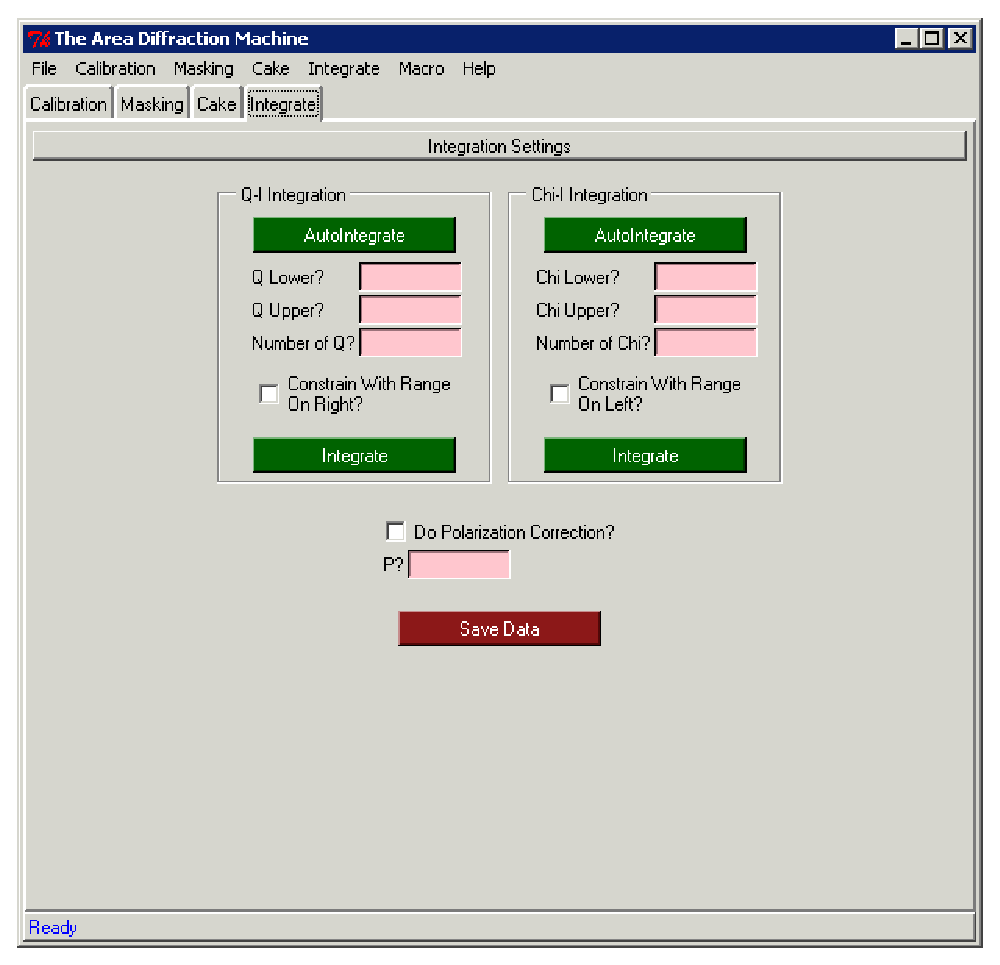
\includegraphics[scale=.75]{figures/integration_page.eps}
\caption{A screen shot of the integration tab to the 
    program. This is the tab where you can integrate data.} 
\label{integration_page}
\end{SCfigure}

To perform a $\chi$ integration, you can use the inputs
on the right under the name \gui{Chi-I Integration}.
The inputs on the right allow you to specify
a range in $\chi$ with the \gui{Chi Lower?} and
\gui{Chi Upper?} inputs. The number of bins in
$\chi$ space can be specified with the
\gui{Number of Chi?} input. To perform the
$\chi$ integration, you have to push the
\gui{Integrate} button on the right.

\section{The Integration Window}

\begin{SCfigure}[1][htb]
\centering
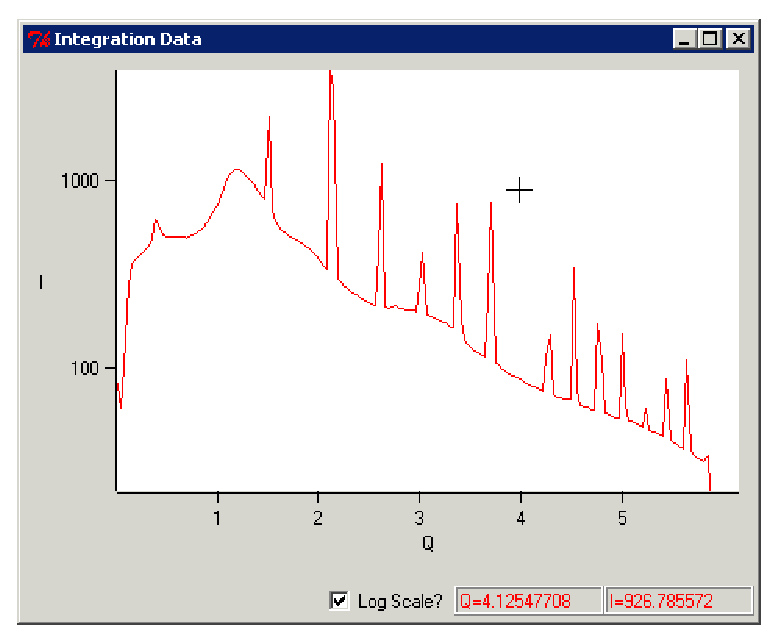
\includegraphics[scale=.75]{figures/integration_window_q.eps}
\caption{A screen shot of the integration window that
    opens up after you perform an intensity integration.} 
\label{integration_window_q}
\end{SCfigure}

\begin{SCfigure}[1][htb]
\centering
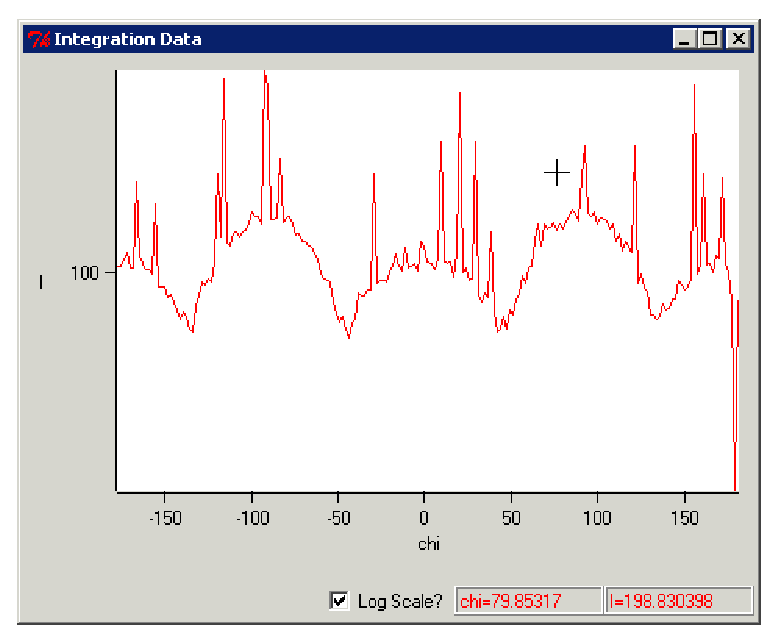
\includegraphics[scale=.75]{figures/integration_window_chi.eps}
\caption{A screen shot of the integration window that
    opens up after you perform an intensity integration.} 
\label{integration_window_chi}
\end{SCfigure}

After you push the integrate button, a line plot of the 
integrated data will be displayed in a new window. 
Figure~\ref{integration_window_q} shows 
the window displaying $Q$ integrated data
and figure~\ref{integration_window_chi} shows the
window displaying $\chi$ integrated ata.
Similar to the diffraction data display and the cake 
data display, this window has a couple of nice featuers
\begin{itemize}
    \item {\em Zoom into the data} - To zoom, left click
    on the data and hold down on the mouse. When you drag 
    the cursor, the program will create a resizing square. 
    When you let go of the mouse, the selected square will 
    be used as the outer bound and the image will be zoomed 
    into it. 
    \item {\em Zoom out of the data} - To unzoom, right
    click on the graph
    \item {\em Resize the window} - This will make the graph
    either larger or smaller. To do so, click on the bottom 
    right corner and drag. 
    \item {\em Read coordinates for a selected point} -
    When you mouse over the graph, the selected $Q$ (or $\chi$
    or $2\theta$) and intensity value will be displayed.
    \item {\em Log Scaling} - The \gui{Log Scale?} check box
    will toggle whether to display a log scale of the data.
\end{itemize}

\section{\texorpdfstring{Working in $2\theta$}{Working in 2theta}}

This program can integrate in $2\theta$ instead of $Q$. To 
do so, you have to go into menu bar up top and select
the \gui{Work in 2theta} option instead of the
\gui{Work in Q} option. Once you do this, the whole program
will just act like it was set to work in $2\theta$ all
along. The labels
on the program will change so that the option will say
\gui{2$\theta$-I Integration}. The other inputs will change
to \gui{2$\theta$ Lower}, \gui{2$\theta$ Upper}, and
\gui{Number of 2$\theta$}. When you push the left
\gui{Integrate} button, the program will integrate 
in $2\theta$ and the window that opens will show a plot
of average intensity as a function of $2\theta$.
If there are any values in the \gui{Q Lower} or
\gui{Q Upper}, they will be convert to $2\theta$
values when the program switches over. If you switch
from $2\theta$ back to $Q$, they will be converted
the other way.

\section{AutoIntegrate}

There is a convenience function similar to the
\gui{AutoCake} button called \gui{AutoIntegrate}. 
\gui{AutoIntegrate} will try to pick a nice range 
and then do the integration. The AutoIntegrate button 
on the left will guess at a nice range of $Q$ 
or $2\theta$ values and then do the $Q$ or
$2\theta$ integration.
It will always make the lower $Q$ or $2\theta$ 
value 0 and the upper value large enough
to include all the data.
It will set the number of $Q$ or $2\theta$ values to
200.

The \gui{AutoIntegrate} button on the right 
will guess a nice range of $\chi$ and then
do the $\chi$ integration. It will always 
set \gui{Chi Lower} to -180, \gui{Chi Upper} to
180, and \gui{Number of Chi} to 200.

\section{Constraining the Inputs}

As was described in the integration algorithm 
section, an integration in one parameter can 
be constrained by another parameter. For example,
a $Q$ or $2\theta$ integration can be done only 
of values in a particular $\chi$ range. Also,
A $\chi$ integration can be done only of a
particular $Q$ or $2\theta$ range. Of course,
it would be meaningless to constrain $Q$ by
$2\theta$.

To constrain the integration using the program,
there are two convenient 
\gui{Constrain With Range On Right?} and 
\gui{Constrain With Range On Left?} check boxes.
When you select
\gui{Constrain With Range On Right?}, the
$Q$ or $2\theta$ integration being done
will be constrained in $\chi$ by range
set with \gui{Chi Lower} and \gui{Chi Upper}.
When you select
\gui{Constrain With Range On Left?}, the
$\chi$ integration will be constrained by
either $Q$ or $2\theta$ (whichever mode the
program is currently in) by the lower and
upper inputs to the left.

\section{Masking}

The program can allows for masking of certain
pixels inside the image. 
Masking of intensity integrated data will be done
whenver the
\gui{Do Greater Than Mask?}, \gui{Do Less Than Mask?},
or \gui{Do Polygon Mask?} check boxes are selected.
Whenever the program finds an intensity value
that you specify should be masked (either because it 
is too large, too small, or in a polygon mask), it makes
sure not to bin that pixel and acts as though
it does not exist. So if you don't want to include
in your integration any values too large or too
small, you can use a threshold mask. If you
don't want to mask any values inside of a certain
region, you can use a polygon mask. 
Refer to Chapter When analyzing diffraction dat, not all of the pixels in 
an image should be used in the analysis. In order to make 
the program
ignore certain pixels when doing the analysis, this
program allows for two types of pixel masking:
threshold masking and polygon masking. You can 
apply either of these from the 
\gui{Masking} tab. figure~\ref{masking_tab}
shows this tab. 

\section{Threshold Masking}

\begin{SCfigure}[1][htbp]
    \centering
    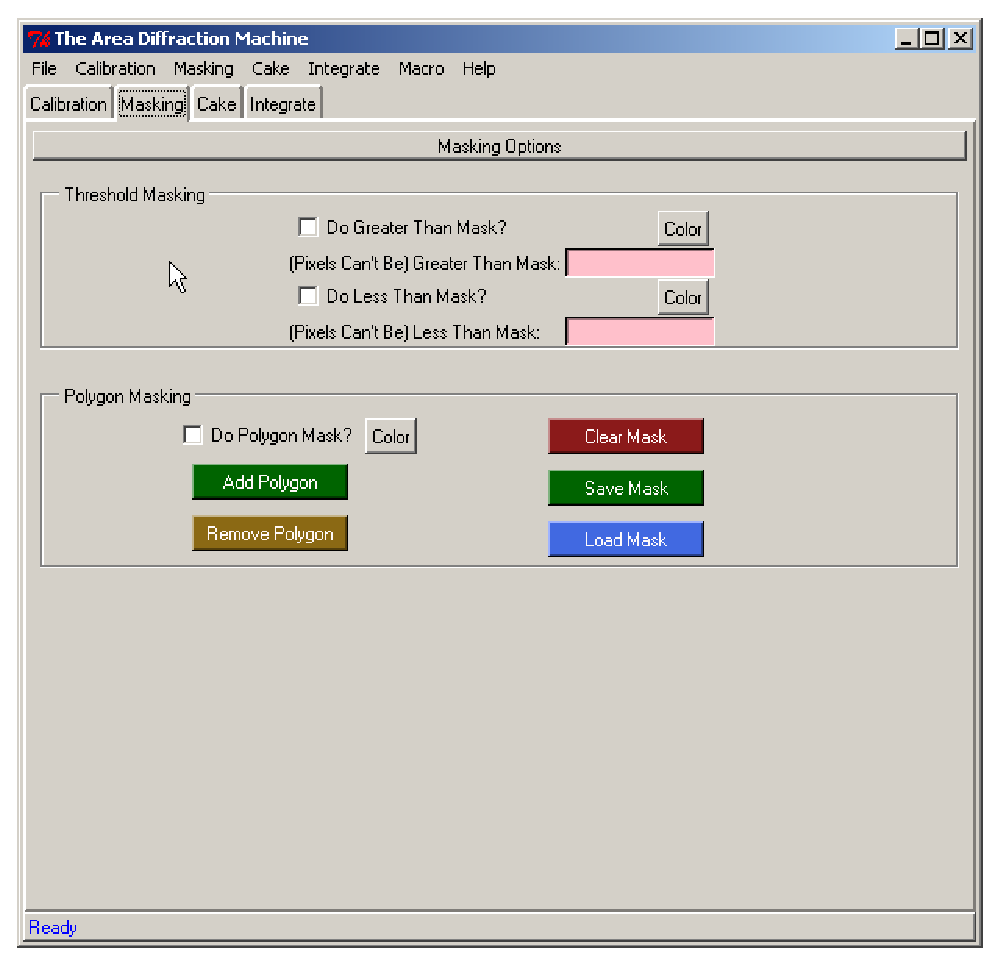
\includegraphics[scale=.75]{figures/masking_tab.eps}
    \caption{The pixel masking tab. It allows for threshold 
    masking and polygon masking.} 
    \label{masking_tab}
\end{SCfigure}

The top half of the \gui{Masking} tab is devoted to 
threshold masking. Threshold masking allows all pixels, 
either above a certain intensity or below a certain 
intensity, to be ignored when doing the diffraction 
analysis. The \gui{Do Greater Than Mask?} check box can 
be used to apply a mask that will cause all pixels 
greater than a certain value to be ignored.
The \gui{(Pixel's Can't Be) Greater Than Mask} input 
can be used to specify the maximum pixel value.
Correspondingly, the \gui{Do Less Than Mask} check box
can be used to make the program ignores all
pixels below a certain value. The particular value can 
be specified with the \gui{Less Than Mask} input. 

\begin{SCfigure}[1][htbp]
    \centering
    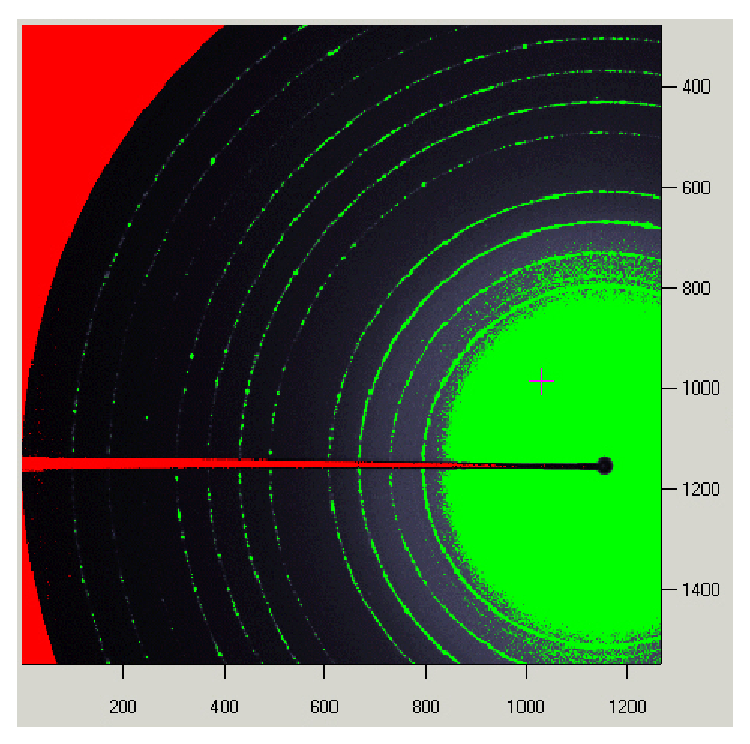
\includegraphics[scale=.75]{figures/Threshold_Masking.eps}
    \caption{A diffraction image with a
    greater than mask and less than mask.
    All pixels with intensity greater than 5000 
    have been colored green. All pixels with 
    intensity less than 30 have been colored red. Applying
    an intensity mask can be a useful way to see if a detector's
    pixels have been overloaded. They can also be a used to
    ensure that no overloaded pixels are used in subsequent
    data analysis.}
    \label{Threshold_Masking}
\end{SCfigure}

When you apply a threshold mask, the pixels over this threshold 
will all be colored differently on the diffraction and cake image. 
You can specify what you want these masked to be colored 
with the \gui{Color} button next to the greater 
than and less then masks. Figure~\ref{Threshold_Masking} shows 
what a diffraction image looks like when all pixels
with intensity above 5000 are colored green and all pixels 
below 30 are colored red.

When caked data is saved out to a file, any of the pixels 
that are larger than the greater than mask are saved 
as -2. Any of the pixels smaller than the less than mask
are saved as -3.  If you need to analyze caked data outside 
the program, this behaviour needs to be accounted for.

When an intensity integration is saved to a file, 
any of the too high or too low pixels are simply ignored when 
calculating average intensity. 

\section{Polygon Masking}

\begin{SCfigure}[1][htbp]
    \centering
    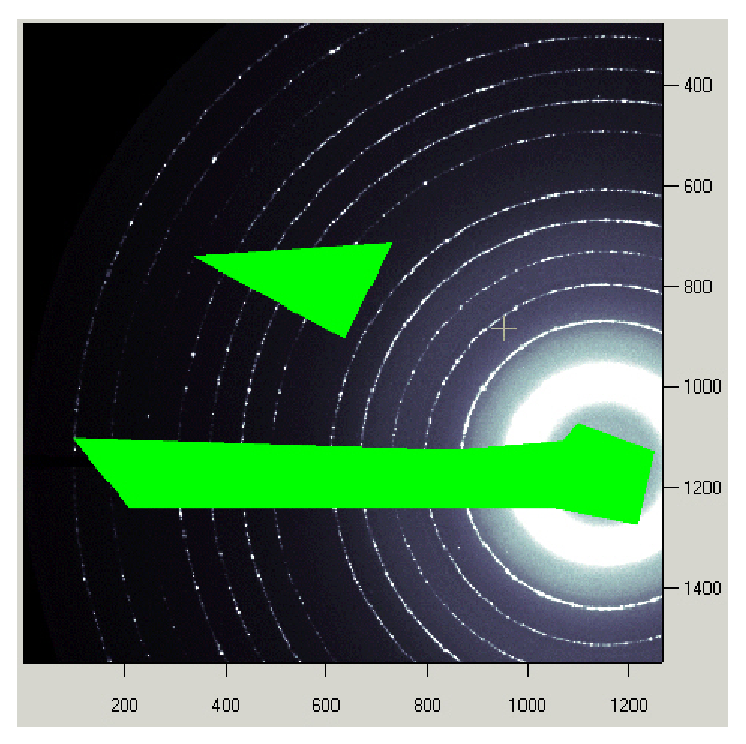
\includegraphics[scale=.75]{figures/Displayed_Polygon.eps}
    \caption{Here are two polygon masks that have been applied
    to a diffraction image. One of them blocks the beam stop.}
    \label{Displayed_Polygon}
\end{SCfigure}

Sometimes, large areas of a diffraction image should not
be included in any data analysis. For example, 
often a beam stop blocks part of the detector
and the pixels behind the beam stop should be ignored. 
To allow for this sort of masking, the program has a 
polygon masking feature. Polygons can be drawn around 
certain parts of the diffraction image and those parts 
of the image will not be used in any subsequent analysis. 
This program can handle multiple polygons at the same time.

So long as the \gui{Do Polygon Mask?} check box is
selected, the polygon masks will be used 
when performing subsequent analysis. 
The polygons will be displayed on the diffraction and cake image. 
Any pixel in the diffraction or cake image that is inside one of
the polygons will have a different color.
An example of polygons on a diffraction image are 
shown in figure~\ref{Displayed_Polygon}.
The color of the polygon masks can be changed using 
using the \gui{Color} button
next to the \gui{Do Polygon Mask?} check box.
When caked data is saved out, any pixels inside 
polygon masks will be given an intensity 
value of -4. During an intensity integration 
masked pixels will be ignored.

\begin{SCfigure}[1][htbp]
    \centering
    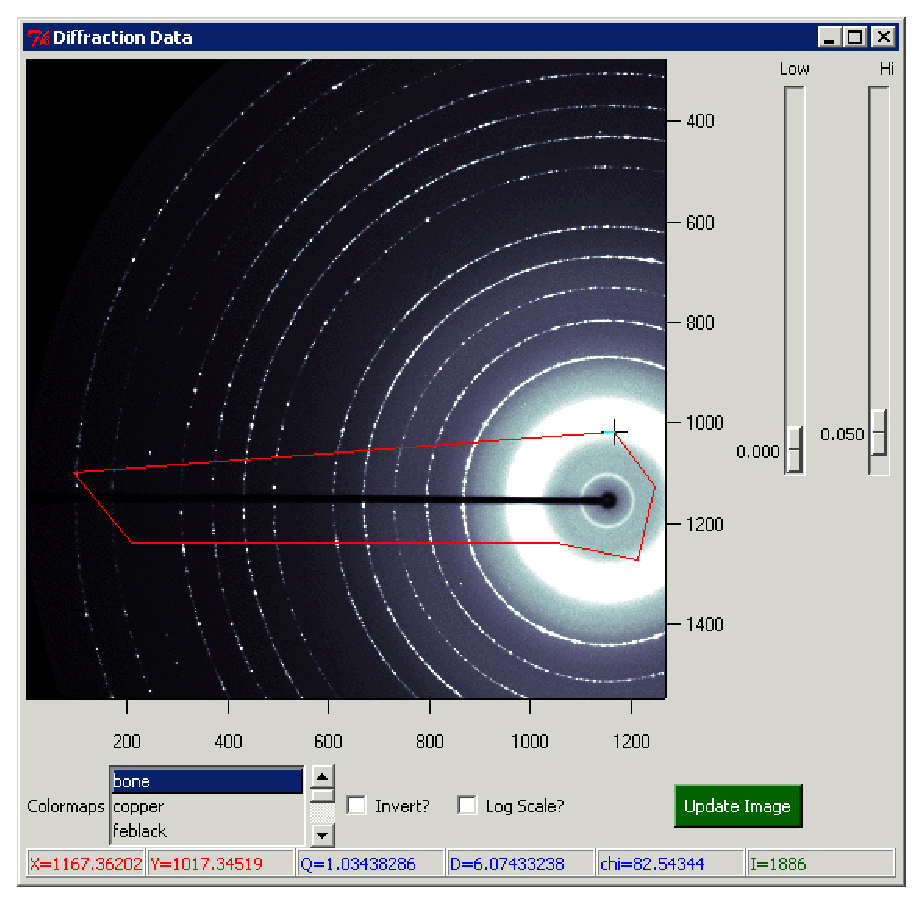
\includegraphics[scale=.75]{figures/Adding_Polygon.eps}
    \caption{Here is the interface for adding a new polygon 
    mask to the program. This particular mask will cover 
    the beam stop so that the beam stop does not affect
    the intensity integration.}
    \label{Adding_Polygon}
\end{SCfigure}

A polygon mask can be added to the image by pushing
the \gui{Add Polygon} button on the \gui{Masking} tab. 
This button will stay down when pushed.  Pushing it puts 
the program in polygon drawing mode.  In this mode, the 
diffraction image will behave differently. The diffraction
image can no longer be zoomed or panned.
Instead, left clicking on the diffraction image will make
the program draw the polygon.  The first left click adds the
first vertex. Each success left click add another vertex. 
The drawing can be finished by right clicking (this will
also create a final vertex). Right clicking will make
the program exit the drawing mode, return to its
original state, and add the polygon into the program. 
Multiple polygons can be added using the \gui{Add Polygon}
button. Figure~\ref{Adding_Polygon} shows 
the program when a polygon is
being drawn. Drawing a polygon can be aborted without
saving the mask by unpushing the \gui{Add Polygon} button.

\begin{SCfigure}[1][htbp]
    \centering
    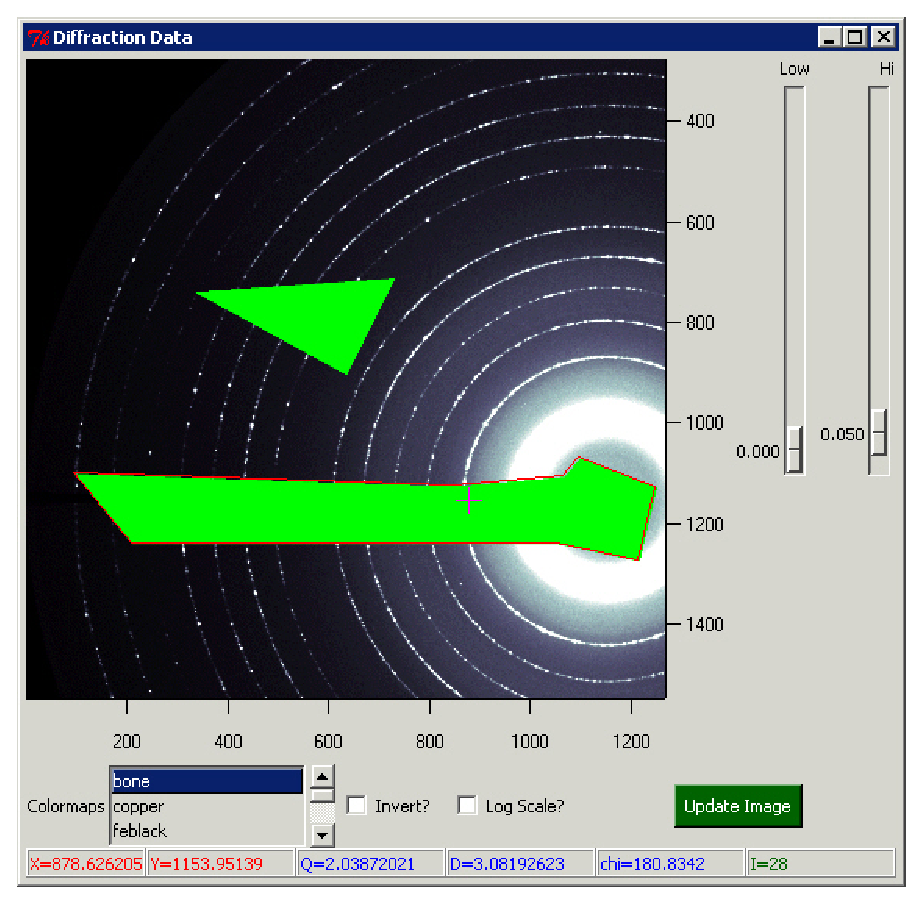
\includegraphics[scale=.75]{figures/Removing_Polygon.eps}
    \caption{Here is the diffraction
    image window as a polygon is about to be removed.
    When mousing over a polygon to remove it,
    the program will display a red border around it.}
    \label{Removing_Polygon}
\end{SCfigure}

The \gui{Remove Polygon} button can be used to remove
a polygon in the program. Like the \gui{Add Polygon} 
button, this button will stay pushed and change the
behavior of the diffraction image. After the 
\gui{Remove Polygon} button is pushed, clicking over
a particular polygon will remove it.
After the polygon is removed, the program will 
return to its normal state.
Figure~\ref{Removing_Polygon} shows what the diffraction
window looks like when a polygon is about to be removed.
The program can be returned to its normal state without
removing a polygon by unpushing the \gui{Remove Polgyon}
button.

The \gui{Clear Mask} button can be used to remove
all the polygons at once. The \gui{Save Mask} button
can be used to save all the polygons to a file.
A file of polygons can be added to the program 
using the 
\gui{Load Mask} button. The file for polygon
files is very simple. For the polygons in 
figure~\ref{Displayed_Polygon}, the following
file would be saved:
\begin{lstlisting}[caption={'polygons.dat'}]
# Polygon(s) drawn on Thu Feb 07 00:00:21 2008
93.140587183	1098.06704199
208.013978042	1237.77792276
1052.48863517	1237.77792276
1213.93231962	1271.92947139
1248.08386825	1126.00921814
1095.95424252	1067.02017959
1064.90738013	1104.27641447
847.579343365	1122.9045319

332.201427619	737.923438212
633.355992844	902.471808902
729.601266267	709.981262058
\end{lstlisting}
Each line is an ($x$,$y$) coordinate for one of 
the nodes of a polygon.  The coordinates are separated
by spaces. Each polygon is separated by a newline.  
Comment lines beginning with \# are 
ignored. 

\section{Masking Caked Plots}

\begin{figure}[htb]
    \centering
    \subfloat[A rectangular polygon mask in 
    the middle of a diffraction image]{
    \label{box_mask_diffraction}
    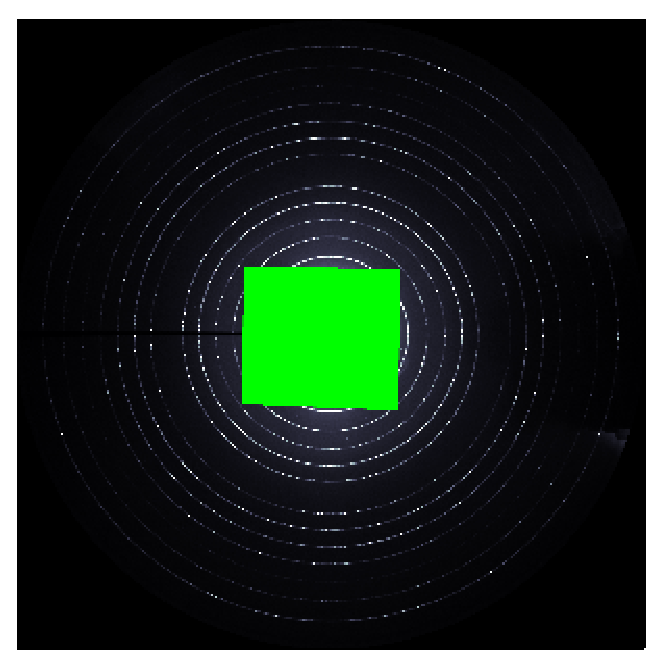
\includegraphics[scale=.75]{figures/box_mask_diffraction_image.eps}}\;\;
    \subfloat[The same rectangular mask on
    a caked plot]{
    \label{box_mask_cake}
    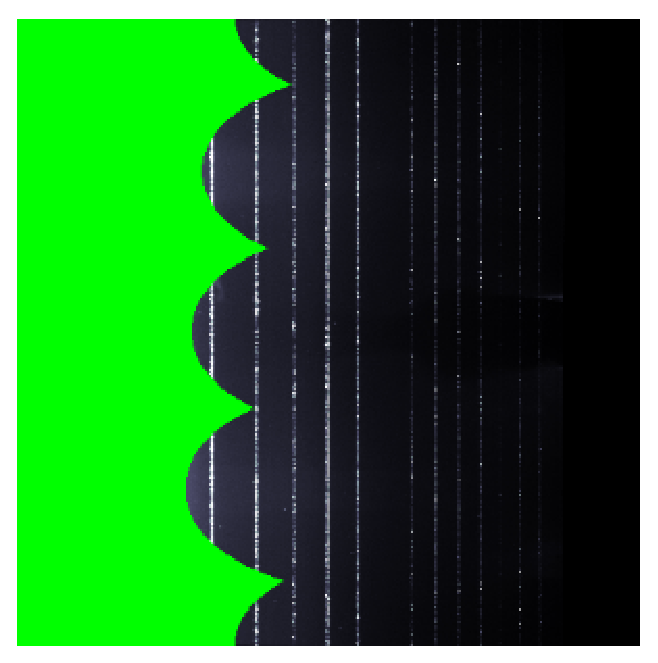
\includegraphics[scale=.75]{figures/box_mask_cake_image.eps}}
    \caption{An example of how a relatively simple
    shape on a diffraction image will can look very
    different on a caked plot.}
    \label{box_mask}
\end{figure}

Any polygon mask or threshold mask will also 
show up on the caked plot. Polygons on the 
diffraction image can look very distorted on 
caked plots. Figure~\ref{box_mask} shows an example.



 for information 
about how to apply a pixel mask.

\section{Saving Integrated Data}

After you have pushed the \gui{Integrate} buton
and performed a $Q$, $2\theta$, or $\chi$ integration,
you can save out the intensity integrated data
using the \gui{Save Data} button. The format of 
an intensity integration data file is as follows:
\begin{lstlisting}[caption={'A Cake Data File'}]
# Q vs I Intensity Integration
# Intensity integration of: C:/data/LaB6_14_02_56.mar3450 
# Data Integrated on Fri Mar 21 17:59:16 2008
# Calibration data used:
#   x center:    1725.0000000 pixels
#   y center:    1725.0000000 pixels
#   distance:     125.2960000 mm
#   energy:     12735.3957721 eV
#   alpha:          0.0000000 degrees
#   beta:           0.0000000 degrees
#   rotation:       0.0000000 degrees
#   pixel length:     100.0000000 microns
#   pixel height:     100.0000000 microns
# A polarization correction was applied
#   P = 1.000000
# A greater than mask was applied
#   Greater than mask = 10000.000000 (All pixels above 10000.000000 were ignored)
# A Less Than Mask was applied.
#   Less than mask = 50.000000 (All pixels below 50.000000 were ignored)
# Polygon mask(s) were applied
# Polygon(s) used in the analysis:
#   647.844364937	1369.72808587
#   1449.93738819	3226.88193202
#   2535.84794275	1449.93738819
#
#   1258.66905188	641.674418605
#   1215.47942755	999.531305903
#   1505.46690519	1116.76028623
#   1653.54561717	777.413237925
# Integration performed with a chi constraint
#   chi constraint lower: 90.000000
#   chi constraint upper: 270.000000
# Integration Range:
#   Q Lower = 0.000000
#   Q Upper = 6.726544
#   Number of Q = 200.000000
#   Q Step = 0.033633
# Q	Avg Intensity
0.016901	0.000000
0.050703	0.000000
0.084504	0.000000
0.118306	0.000000
0.152108	0.000000
0.185910	0.000000
...
\end{lstlisting}
The header is a bunch of lines that begin with \#.
Each line says something useful about the state
of the program when the integratinon was
done. 
If you perform an intensity integration in $\chi$
space instead, the header file will say
\macroline{\# Chi vs I Intensity Integration}
If two files were added together
and then integrated, the header file will say
\begin{lstlisting}[caption={'Alternate Header'}]
# Intensity integration of: C:/first.mar3450 C:/first.mar3450
\end{lstlisting}
Follwing the header string is the line
\macroline{\# Q Avg Intensity} (or \macroline{\# Chi Avg Intensity}
or \macroline{\# 2theta	Avg Intensity}). Following it is
the data. Each line contains one of the bins. The data
is tab seperated. The first number is the middle $Q$ (or
$\chi$ or $2\theta$ value) in the bin and the second number
is the average intensity.





The macro file format is pretty simple. A macro file contains many commands which automates the GUI. Each command in the GUI gets its own line. Each command has a fairly straightforward style. If you want to do something to the GUI, you look at the name on top of the thing or near the thing and macro command is exactly that string. This sounds confusing but it is not too bad. If you want to get the calibration data from the header of the image, the macro line is \macroline{Get From Header}. If you want to fit the calibration data, the macro line is \macroline{Do Fit}.

Things get more interesting when what you want to do requires doing more then just pushing a button. For example, if you want to deselect the \gui{Draw Q Data?} checkbox, your macro needs to specify that you deselect this option instead of selecting it. To dos this, the first part of the macro command is the name of the checkbox \macroline{Cake} and the next line tells you what you want to do with it. Your macro would contain these lines:
\begin{lstlisting}[caption={'Draw the $Q$ Lines on the Display'}]
Draw Q Data?
    Select
# Or, to not display them:
Draw Q Data?
    Deselect
\end{lstlisting}
The exact same format is used for user input. To change the calibration values, your macro file would look like:
\begin{lstlisting}[caption={'Input a Number'}]
xc:
    1752.3
beta:
    5.23
\end{lstlisting}
Finally, some of the Gui commands require a file name. For example, you must provide a file name to load a diffraction file or save a caked image. Whenever the command has a required file, the next line in the macro file should be that file name. For example, if you wantd to save the cake image, your macro file would contain the line: 
\begin{lstlisting}[caption={'Save the Caked Image'}]
Save Caked Image
    C:/data/cake_output.jpg
\end{lstlisting}

If you look at the first page, there are three inputs: \gui{Get From Header:}, \gui{dark current:}, and \gui{Q data:}. The macro command to load any of these is a little bit ambiguous. When using the acutal GUI, you would, at least in principle, type in the name of a file and then press load. But there is no reason to make the GUI so redundant. So to load in any of these using a macro command, all you have to do is give the name of the input and then the filename. It will automatically load the file without you explicitly giving the \macroline{load} line. So, for example, to load in the $Q$ data, you would include the following lines:
\begin{lstlisting}[caption={'Load the $Q$ Data'}]
Q Data:
    C:/data/q_data.dat
\end{lstlisting}

\subsection{Looping Over Diffraction Data}
Suppose you want to do the same general analysis to many diffraction files at the same time. There is an easy way to do this. To analize one file at a time, you would simply issue the command
\begin{lstlisting}[caption={'Load the Diffraction Data'}]
Load Data:
    C:/data/first.mar3450
Integrate Q Lower?
    .25
Integrate Q-I
# ...
\end{lstlisting}
To loop over multiple diffraction images at once, you could simply give more files after the first one. You can even give it whole directories. When you give it a directory to loop over, the program will (non-recursively) look for all the diffraction files in that directory and include them in the list. Just make sure to put all the files on the same line. The loop will end when one of the 3 things in the macro file happens. Either, a subsequent line in the macro file reads \macroline{END LOOP}, more diffraction data is loaded using the command \macroline{Load Data:}, or the macro file ends. For example, if we look at this macro file.
\begin{lstlisting}[caption={'Loop Over Diffraction Data'}]
Load Data:
    C:/data/first.mar3450 C:/data/second_file.mar3450 
Integrate Q Lower?
    .25
Integrate Q-I
END_LOOP
Draw Q Lines?
    Select
# ...
\end{lstlisting}
We see that it would get evaluated exactly like the following macro file:
\begin{lstlisting}[caption={'An Equivalent Macro'}]
Load Data:
    C:/data/first.mar3450 
Integrate Q Lower?
    .25
Integrate Q-I
Load Data:
    C:/data/second.mar3450 
Integrate Q Lower?
    .25
Integrate Q-I
Draw Q Lines?
    Select
# ...
\end{lstlisting}

Finally, there is a convenience markup which can help you make fancy macros. Whenever you have loaded data in, you can refer to the part name of the current diffraction file that is loaded using the string \macroline{PATHNAME} and you can refer to the file name itself using the string \macroline{FILENAME}. So, in our previous example, if we had loaded the file \macroline{C:/data/second\_file.mar3450}, \macroline{PATHNAME} would get chaned into \macroline{C:/data} and \macroline{PATHNAME} would get evaluated to \macroline{second\_file} without the extension. In effect, you can imagine building back the full name from \macroline{PATHNAME} and \macroline{FILENAME} using an equation line
\begin{equation*}
\text{\macrolinenoquotes{C:/data/second\_file.mar3450}=\macrolinenoquotes{FILENAME/PATHNAME.mar3450}}
\end{equation*}
These commands are useful because they allow you to loop over many files at once but still save things in useful places and with useful names. It would be easy, for example, to save the intensity data you calculate for each file being looped over using the macro command:
\begin{lstlisting}[caption={'Using the FILENAME and PATHNAME Markup'}]
Save Integration Data
    FILENAME/PATHNAME\_intensity.dat
\end{lstlisting}
This would save, for example, \macroline{C:/data/first.mar3450}'s intensity data to \macroline{C:/data/first\_intensity.dat}, \macroline{C:/data/second.mar3450}'s intensity data to \macroline{C:/data/second\_intensity.dat}, and the same for all the others. This feature lets you have the macro to save each of the files to the right place and give it a useful name.

\subsection{A More Interesting Example}

\begin{lstlisting}[caption={'A Non-Trivial Macro'}]
# Macro file to calibrate from one file and 
# then analyze many others
Data File:
    C:\data\calibration\cal.mar3450
Get From Header
# Fix the energy before doing the fit
E Fixed
    Select
Number of chi?
    150
stddev?
    8
# This would be standard Q values for the sample
Q Data:
    S:\data\calibration\Q_data.dat
Do Fit
Save Calibration
    C:\data\calibration\cal_values.dat
Draw Q lines?
    Select
Draw Peaks?
    Select
AutoCake
Cake Data Hi
    0.03
Save Caked Image
    C:\data\calibration\cal_cake.jpg
# Load in a directory of data to analyze
Data File:
    S:\data\to_analyze\
Integrate Q Lower?
    .25
Integrate Q Upper?
    4.5
Integrate Number of Q?
    500
Integrate Q-I data
Save Integration Data
    PATHNAME\FILENAME_Q_I_integration.dat
\end{lstlisting}

The macro first moves the GUI to the calibration tab. It then loads in a calibration image, $Q$ data, and uses as the initial guess for the calibration values number in the header of the file. It then does the fit and saves the fit calibration values to a file.  It then cakes the data and saves a cake of this calibration with the $Q$ lines and Peaks so that later visual inspection can show how good the fit was. Afterwards, it loops over a directory of diffraction dat and, using the same calibration data, sets the $Q$ range of the intensity integration, does the intensity integration, and saves integrated data next to the corresponding diffraction files. It should now be apparent that macro are both fun and easy.

     
\subsection{Little Tidbits}\label{Little Tidbits}
\begin{itemize}
\item Any of the macro commands themselves are case insensitive. The command \macroline{GeT fRoM hEaDeR} is just as valid as the command \macroline{gET fROM hEADER} and \macroline{Get From Header}. You don't have to sweat it. 
\item White spaces at the beginning and end of the line are ignored. In the preceding examples, the spaces separating macro commands from input values such as file names are there only to increase readability. You don't need them if you don't want.
\item New lines are ignored
\item comment lines of the form \macroline{\# This would be a comment} are ignored.
\item You don't have to worry about explicitly moving from tab to tab in the computer program. The computer program will move to the right automatically before performs the action.
\item When you issue the macro command \macroline{E:} or \macroline{E Fixed}, the computer program will automatically set the GUI to \macroline{Work in eV}. If you issue the command or \macroline{lambda:} or \macroline{lambda fixed:} then the comptuer program will set the GUI to \macroline{Work in Lambda}. You can also explicitly set the GUI to either mode using the commadn \macroline{Work in eV} or \macroline{Work in Lambda}.
\item I need to figure out what colors are allowed.
\end{itemize}

%Command&Followed By&Description\\

\subsection{Macro Commands}


\begin{center}

\setlongtables % keeps the width uniform across both pages
\begin{longtable}{|p{3cm}|p{4cm}|p{7cm}|}
%\begin{longtable}{|l|l|l|}
\caption{Macro Commands} \label{grid_mlmmh} \\

\hline \multicolumn{1}{|c|}{Command} & \multicolumn{1}{c|}{Followed By} & \multicolumn{1}{c|}{Effect} \\ \hline 
\endfirsthead

\multicolumn{3}{c}%
{{\bfseries \tablename\ \thetable{} -- continued from previous page}} \\

\hline \multicolumn{1}{|c|}{Command} & \multicolumn{1}{c|}{Followed By} & \multicolumn{1}{c|}{Effect} \\ \hline 
\endhead

\hline \multicolumn{3}{|r|}{{Continued on next page}} \\ \hline
\endfoot

\hline 
\endlastfoot
\multicolumn{3}{|l|}{Calibration Values} \\
\hline
\macrolinenoquotes{Data File:}&Filename(s) and/or Directory(s)&Loops over loading in each file\\
\macrolinenoquotes{Dark Current:}&Filename&Loads in the Dark Current \\
\macrolinenoquotes{Q Data:}&Filename&Load in the $Q$ data\\
\macrolinenoquotes{Get From Header:}&None&Sets the calibration data to the value stored in the image header.\\
\macrolinenoquotes{Load From File:}&Filename&Loads a calibration data file.\\
\macrolinenoquotes{Previous Values}&None&Loads the previously stored calibration values.\\
\macrolinenoquotes{Save To File}&Filename&Saves the calibration data to a file.\\
\macrolinenoquotes{xc:}&Number&Sets the $x$ center.\\
\macrolinenoquotes{xc Fixed:} & \selectordeselect & Sets whether or not to fix the $x$ center while doing the fit.\\
\macrolinenoquotes{yc:}&Number&Set the $y$ center.\\
\macrolinenoquotes{yc Fixed:}& \selectordeselect &Sets whether or not to fix the $y$ center while doing the fit.\\
\macrolinenoquotes{d:}&Number&Set the distance.\\
\macrolinenoquotes{d Fixed:}& \selectordeselect &Sets whether or not to fix the distance while doing the fit.\\
\macrolinenoquotes{E:}&Number&Sets the energy.\\
\macrolinenoquotes{E Fixed:}& \selectordeselect &Sets whether or not to fix the energy while doing the fit.\\
\macrolinenoquotes{lambda:}&Number&Sets the wavelength.\\
\macrolinenoquotes{lambda Fixed:}& \selectordeselect &Sets whether or not to fix the wavelength while doing the fit.\\
\macrolinenoquotes{alpha:}&Number&Sets the $\alpha$ angle.\\
\macrolinenoquotes{alpha Fixed:}& \selectordeselect &Sets whether or not to fix the $\alpha$ angle while doing the fit.\\
\macrolinenoquotes{beta:}&Number&Sets the $\beta$ angle.\\
\macrolinenoquotes{beta Fixed:}& \selectordeselect &Sets whether or not to fix the $\beta$ angle while doing the fit.\\
\macrolinenoquotes{R:}&Number&Sets the rotation angle.\\
\macrolinenoquotes{R Fixed:}& \selectordeselect &Sets whether or not to fix the rotation angle while doing the fit.\\
\macrolinenoquotes{Draw Q Lines?}&\selectordeselect&Sets wether or not to draw constant $Q$ lines on the screen.\\
\macrolinenoquotes{Draw Q Lines Color?}&A color&Sets the color of the constant $Q$ lines\\
\macrolinenoquotes{Draw dQ Lines?}&\selectordeselect&Draw the delta $Q$ lines on the diffraction image\\
\macrolinenoquotes{Draw dQ Lines Color?}&A color&Change the color of the delta $Q$ lines\\
\macrolinenoquotes{Draw Peaks?}&\selectordeselect&Draw the fit peaks on the diffraction and cake image\\
\macrolinenoquotes{Draw Peaks Color?}&A color&Change the color of the peaks\\
\macrolinenoquotes{Update}&None&Update the diffraction image\\
\macrolinenoquotes{Do Fit}&None&Fit the calibration values to a loaded diffraction image\\
\macrolinenoquotes{Make/Save Peak List}&Filename&Creates a peak list just as happens when doing the fit, but instead of acutally doing the fit it saves the peaks as an ASCII file for later use.\\
\macrolinenoquotes{Use Old Peak List (if possible)?}&\selectordeselect&Uses the previously found peak list again when doing the fit.\\
\macrolinenoquotes{Number of Chi?}&Value&The number of $\chi$ slices around the diffraction image to pick and use when doing the calibration\\
\macrolinenoquotes{Stddev}&Value&The $\sigma$ threshold for allowing a peak.\\
\hline    
\multicolumn{3}{|l|}{Diffraction Display Options} \\
\hline
\macrolinenoquotes{Diffraction Data Colormaps}&A colormap name&Select the color map to use for the diffraction image.\\
\macrolinenoquotes{Diffraction Data Invert?}&\selectordeselect&Invert the color map that is being used\\
\macrolinenoquotes{Diffraction Data Log Scale?}&\selectordeselect&Take the log of all the data points before displaying them.\\
\macrolinenoquotes{Diffraction Data Low?}&Value from 0 to 1&The normalized intensity value which will be scaled to \%0 of the image brightness when displaying the diffraction image.\\
\macrolinenoquotes{Diffraction Data Hi?}&Value from 0 to 1&The normalized intensity value which will be scaled to \%100 of the image brightness when displaying the diffraction image.\\
\macrolinenoquotes{Save Diffraction Image}&Filename&Save the diffraction image to a file (possibly including $Q$ lines and peaks.\\
\macrolinenoquotes{Work in eV}&\selectordeselect&Change the GUI to deal with energy in units of eV\\
\macrolinenoquotes{Work in Lambda}&\selectordeselect&Change the GUI to deal with energy in units of $\lambda$ using the conversion $E=hc/\lambda$.\\
\hline    
\multicolumn{3}{|l|}{Cake Macro Commands}\\
\hline
\macrolinenoquotes{AutoCake}&None&Make the computer pick a nice $Q$ and $\chi$ range and Cake the data.\\
\macrolinenoquotes{Cake Q Lower?}&Value&The lower $Q$ value of the caked data.\\
\macrolinenoquotes{Cake Q Upper?}&Value&The upper $Q$ value of the caked data.\\
\macrolinenoquotes{Cake Number of Q?}&Value&The number of $Q$ bins to use while caking the data.\\
\macrolinenoquotes{Cake Chi Lower?}&Value&The lower $\chi$ value of the caked data.\\
\macrolinenoquotes{Cake Chi Upper?}&Value&The upper $\chi$ value of the caked data.\\
\macrolinenoquotes{Cake Number of Chi?}&Value&The number of $\chi$ bins to use while caking the data.\\
\macrolinenoquotes{Do Cake}&None&Cake the data.\\
\macrolinenoquotes{Last Cake}&None&Go back to the previous cake values.\\
\macrolinenoquotes{Save Caked Image}&Filename&\\
\macrolinenoquotes{Save Caked Data}&Filename&\\
\hline    
\multicolumn{3}{|l|}{Cake Display Options} \\
\hline
\macrolinenoquotes{Cake Data Colormaps:}&Colormap&\\
\macrolinenoquotes{Cake Data Invert?}&\selectordeselect&\\
\macrolinenoquotes{Cake Data Log Scale?}&\selectordeselect&\\
\macrolinenoquotes{Cake Data Low}&&\\
\macrolinenoquotes{Cake Data Hi}&&\\
\hline    
\multicolumn{3}{|l|}{Intensity Integration Macro Commands}\\
\hline
\macrolinenoquotes{Integrate Q Lower?}&&\\
\macrolinenoquotes{Integrate Q Upper?}&&\\
\macrolinenoquotes{Integrate Number of Q?}&&\\
\macrolinenoquotes{Integrate Chi Lower?}&&\\
\macrolinenoquotes{Integrate Chi Upper?}&&\\
\macrolinenoquotes{Integrate Number of Chi?}&&\\
\macrolinenoquotes{Integrate Q-I Data}&&\\
\macrolinenoquotes{Integrate Chi-I Data}&&\\
\macrolinenoquotes{Save Integration Data}&&\\
\end{longtable}
\end{center}

\subsection{What You Can't Do With Macros}

Just to be clear:
\begin{itemize}
\item There is no way with a macro to zoom into the diffraction data, the cake data, or the intensity integrated data
\item You can't draw individual polygon masks and you can't remove individual polygon masks. All you can do is load in polygon's from file and save all the current polygons to a file.
\item Currently, you cannot load in and add together multiple images using the macro. I indent to code up this feature at some point. 
\end{itemize}



\chapter{The Preferences Page}

In the \gui{File} menu is a \gui{Preferences} option 
which will open a \gui{Preferences} page.

\begin{SCfigure}[1][bthp]
    \centering
    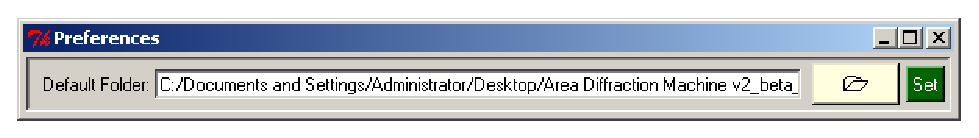
\includegraphics[scale=.75]{figures/preferences_page.eps}
    \caption{The \gui{Preferences} page.}
    \label{divide_up_image}
\end{SCfigure}

\section{Setting the Default Folder}

Currently, the \gui{Preferences} page contains only one input 
\gui{Default Folder} that can be used to set a default folder to
look in when selecting files. Either type in the folder name and push
the \gui{Set} button or simply select the folder from the folder selector
by pushing the button with the folder icon on it. The default folder 
will be persistent. The next time the program is opened, the same default 
folder will be in the input and the program will look in the same default
folder. It does so by saving the folder name in a file named 
\gui{DefaultDirectory.dat} in the folder \gui{Preferences/}.
To make the program not use a default folder, 
simply clear out the input and push the \gui{Set} button.
You can also clear out the default folder by deleting the 
\gui{DefaultDirectory.dat} file in the \gui{Preferences/} folder.





\chapter{Software Licensing}

This program is released under the GNU General
Public License (GPL) version 2.\index{GNU}\index{GPL}
The license can e found at 
\url{http://www.gnu.org/licenses/old-licenses/gpl-2.0.html}.
For the most part, you are free to use and distribute 
this software. You are free to make any modifications to 
the code under the condition that any modifications are clearly 
stated and that the modifications are released under the 
GPL version 2.

This software manual is also licensed under the GPL. 
This is a bit unconventional. I decided to do so after reading
several discussions online. Following Nathanael Nerode's 
article {\em Why You Shouldn't Use the GNU FDL}, I include 
the clarification ``for the purpose of applying the GPL to 
this document, I consider `source code' to refer to the texinfo 
source and `object code' to refer to the generated info, tex, 
dvi, [pdf] and postscript files.''\cite{Nerode03}

This program uses the software package
levmar for performing Levenberg-Marquardt nonlinear
least squares minimization.
\index{Least Squares Minimization}\index{Fitting}
It is released under the GPL. That package can be 
found at \url{http://www.ics.forth.gr/~lourakis/levmar/}.\cite{lourakis04LM}

This program uses the function get\_pck() from the CCP4 package
\index{CCP4}\index{get\_pck()}\index{Mar2300}\index{Mar3450}
DiffractionImage to uncompress Mar data. It
written by Dr. Claudio Klein.\cite{Klein95} 
This prgoram also uses the file marccd\_header.h form
the DiffractionImage packate. It
released under the GPL and can be found at
\url{http://www.ccp4.ac.uk/ccp4bin/viewcvs/ccp4/lib/DiffractionImage/}.\cite{DiffractionImage}

This program uses the EdfFile library (EdfFile.py) for reading and 
writing files of the ESRF Data Format. It is is part of the PyMCA 
library and is licensed under the GNU GPL version 2.\cite{PyMCA}

\index{Polygon Inclusion Testing}
This program also uses W. Randolph Frankin's pnpoly() 
function for performing a point inclusion in polygon test. 
This code can be found at
\url{http://www.ecse.rpi.edu/Homepages/wrf/Research/Short\_Notes/pnpoly.html}
We are in compliance with his software license which is 
reproduced below\cite{Franklin05}:
\begin{quotation}\em
Copyright (c) 1970-2003, Wm. Randolph Franklin

Permission is hereby granted, free of charge, to any person obtaining 
a copy of this software and associated documentation files (the 
``Software''), to deal in the Software without restriction, including 
without limitation the rights to use, copy, modify, merge, publish, 
distribute, sublicense, and/or sell copies of the Software, and to 
permit persons to whom the Software is furnished to do so, subject 
to the following conditions:

Redistributions of source code must retain the above copyright 
notice, this list of conditions and the following disclaimers.
Redistributions in binary form must reproduce the above copyright 
notice in the documentation and/or other materials provided with 
the distribution.
The name of W. Randolph Franklin may not be used to endorse or 
promote products derived from this Software without specific 
prior written permission.
THE SOFTWARE IS PROVIDED ``AS IS'', WITHOUT WARRANTY OF ANY KIND, 
EXPRESS OR IMPLIED, INCLUDING BUT NOT LIMITED TO THE WARRANTIES OF 
MERCHANTABILITY, FITNESS FOR A PARTICULAR PURPOSE AND 
NONINFRINGEMENT. IN NO EVENT SHALL THE AUTHORS OR COPYRIGHT HOLDERS 
BE LIABLE FOR ANY CLAIM, DAMAGES OR OTHER LIABILITY, WHETHER IN AN 
ACTION OF CONTRACT, TORT OR OTHERWISE, ARISING FROM, OUT OF OR IN 
CONNECTION WITH THE SOFTWARE OR THE USE OR OTHER DEALINGS IN THE 
SOFTWARE.
\end{quotation}



% include both bibliographies
\bibliographystyle{plain}
\bibliography{AreaDiffractionMachineManual} 

\printindex

\end{document}


